\documentclass[sigconf]{acmart}
\settopmatter{printacmref=false} % Removes citation information below abstract
%\renewcommand\footnotetextcopyrightpermission[1]{} % removes footnote with conference information in first column

\pagestyle{plain} % removes running headers
\usepackage{booktabs} % For formal tables
\usepackage[T1]{fontenc}
\usepackage{lmodern}
\usepackage{amsmath}
\usepackage{graphicx,subcaption}
\usepackage[ruled,linesnumbered]{algorithm2e}
\DontPrintSemicolon

\newcommand{\eat}[1]{}
\newcommand{\mas}[1]{{\color{red} #1}}
\newcommand{\note}[1]{{\color{blue} #1}}

\newtheorem{definition}{Definition}
\newtheorem{example}{Example}

%\settopmatter{printacmref=false}

% Copyright
%\setcopyright{none}
%\setcopyright{acmcopyright}
%\setcopyright{acmlicensed}
%\setcopyright{rightsretained}
%\setcopyright{usgov}
%\setcopyright{usgovmixed}
%\setcopyright{cagov}
%\setcopyright{cagovmixed}


% DOI
\acmDOI{10.475/123_4}
%
%% ISBN
\acmISBN{123-4567-24-567/08/06}

%Conference
\acmConference[CIKM '18]{ACMconference}{October 2018}{}
\acmYear{2018}
\copyrightyear{2018}
%
%
%\acmArticle{4}
%\acmPrice{15.00}

% These commands are optional
%\acmBooktitle{Transactions of the ACM Woodstock conference}
%\editor{Jennifer B. Sartor}
%\editor{Theo D'Hondt}
%\editor{Wolfgang De Meuter}

%\setcopyright{none}
% uncomment if you want to disablle setcopyright ACM

\begin{document}
\title{DiVE: Diversifiying View Recommendation for Visual Data Exploration}
%\titlenote{Produces the permission block, and
%  copyright information}
%\subtitle{Extended Abstract}
%\subtitlenote{The full version of the author's guide is available as
%  \texttt{acmart.pdf} document}


%\author{Rischan Mafrur}
%\affiliation{%
%  \institution{The University of Queensland}
%  \city{Queensland}
%  \state{Australia}
%}
%\email{r.mafrur@uq.edu.au}
%
%\author{Mohamed A Sharaf}
%\affiliation{%
%	\institution{The University of Queensland}
%	\city{Queensland}
%	\state{Australia}
%}
%\email{m.sharaf@uq.edu.au}

%\author{Hina A Khan}
%\affiliation{%
%	\institution{The University of Queensland}
%	\city{Queensland}
%	\state{Australia}
%}
%\email{h.khan3@uq.edu.au}



% The default list of authors is too long for headers.
%\renewcommand{\shortauthors}{R. Mafrur et al.}
\newcommand{\quotes}[1]{``#1''}

\begin{abstract}

To support effective data exploration, there has been a growing interest in developing solutions that can automatically recommend data visualizations that reveal interesting and useful data-driven insights.
%%
In such solutions, a large number of possible data visualization views are generated and ranked according to some metric of importance (e.g., a deviation-based metric), then the top-k most important views are recommended. 
%%
However, one drawback of that approach is that it often recommends similar views, leaving the data analyst with a limited amount of gained insights.    
%%
To address that limitation, in this work we posit that employing diversification techniques in the process of view recommendation allows eliminating that redundancy and provides a good and concise coverage of the possible insights to be discovered.  
%%
To that end, we propose a hybrid objective utility function, which captures both the importance, as well as the diversity of the insights revealed by the recommended views.
%%
While in principle, traditional diversification methods (e.g., Greedy Construction) provide plausible solutions under our proposed utility function, they suffer from a significantly high query processing cost. 
%
In particular, directly applying such methods leads to a ``process-first-diversify-next" approach, in which all possible data visualization are generated first via executing a large number of aggregate queries. 
%
To address that challenge, we propose an integrated scheme called {\em DiVE}, which efficiently selects the top-k recommended view based on our hybrid utility function.
%
{\em DiVE} leverages the properties of both the importance and diversity metrics to prune a large number of query executions without compromising the quality of recommendations.
%
Our experimental evaluation on real datasets shows the performance gains provided by DiVE.


\eat{
To support effective data exploration, there has been a growing interest in developing solutions that can automatically recommend data visualizations that reveal interesting and useful data-driven insights.
%%
In such solutions, a large number of possible data visualization views are generated and ranked according to some metric of importance (e.g., a deviation-based metric), then the top-k most important views are recommended. 
%%
However, one drawback of that approach is that it often recommends similar views, leaving the data analyst with a limited amount of gained insights.    
%%
To address that limitation, in this work we posit that employing diversification techniques in the process of view recommendation allows eliminating that redundancy and provides a good and concise coverage of the possible insights to be discovered.  
%%
To that end, we propose a hybrid objective utility function, which captures both the importance, as well as the diversity of the insights revealed by the recommended views.
%%


However, such visualizations come at the expense of high data processing costs, where a large number of views are generated to evaluate their usefulness. Those costs are further escalated in the presence of numerical dimensional attributes, due to the potentially large number of possible binning aggregations, which lead to a drastic increase in the number of possible visualizations. 

To address that challenge, in this paper we propose the MuVE scheme for Multi-Objective View Recommendation for Visual Data Exploration. MuVE introduces a hybrid multi-objective utility function, which captures the impact of binning on the utility of visualizations. Consequently, novel algorithms are proposed for the efficient recommendation of data visualizations that are based on numerical dimensions. The main idea underlying MuVE is to incrementally and progressively assess the different benefits provided by a visualization, which allows an early pruning of a large number of unnecessary op- erations. Our extensive experimental results show the significant gains provided by our proposed scheme.

Data visualization is gaining growing interest as an indis- pensable tool for data exploration and analysis in a widely diverse set of discovery-oriented applications [9], [23]. In such applications, data analysts explore large volumes of data look- ing for interesting visualization that reveal new and valuable insights. Such process is typically ad-hoc and labor-intensive, especially for high-dimensional databases. Motivated by the need for efficient data analysis and exploration, several solu- tions for recommending visualizations have recently emerged to guide analysts throughout that rather time-consuming pro- cess (e.g., [22], [21], [14], [13]).



Data visualization, which transforms data into im- ages to make nearly anyone easily understand the data, is invaluable for explaining the significance of data to people who are more visually oriented. The central task of automatic data visualization is, for a given dataset, to visualize its compelling stories by transforming the data (for example, selecting attributes, grouping and binning values) and deciding the right type of visualization (for example, bar charts or line charts).

Technically speaking, �interesting� charts can be defined from three angles: (1) Deviation-based: a chart that is dramat- ically different from the other charts (e.g., SeeDB [22]);
}

\iffalse
\mas{
Today, visualization recommendation tools have become essential part for the easy-to-use visual data exploration systems of large high dimensional datasets. 
%%
Most of the existing research on visualization recommendation focuses on ranking the visualizations on the basis of particular criteria of importance. 
%%
The user is then presented with top-k most important views. 
%%
The limitation of using only importance as ranking criteria is that it often leads to generate redundant views which reveal similar information about the dataset.  
%%
However, a diverse set of recommended views is likely to be more informative than a monotonous set of views due to it able to present representative results. 
%%
Meanwhile, the benefits of visualization recommendation are achieved at the expense of high costs where a large number of all possible views are generated to gain top-k views. 
%%
To address that challenge, in this paper, we propose an integrated scheme called \textit{DiVE}, that evaluates top-k views based on both importance and diversity. 
%%
Towards that end, we propose a combined objective function based on diversity and importance to evaluate the effectiveness of top-k views. 
%%
Further, \textit{DiVE} leverages the properties of the combined objective function to significantly reduce the processing cost of computing top-k views by pruning of a large number of query executions. 
%%
Instead of following the current technique in diversification which is \textit{process-first-diversify-next}, \textit{DiVE} uses the opposite approach that able to prune more than 40 percent of the number of queries. 
%%
We have evaluated the effectiveness and efficiency of our proposed scheme on real datasets. Our experimental results show substantial benefits of our scheme over the state of the art techniques.
}
\fi
% \footnote{This is an abstract footnote}
\end{abstract}

%
% The code below should be generated by the tool at
% http://dl.acm.org/ccs.cfm
% Please copy and paste the code instead of the example below.
%
\begin{CCSXML}
<ccs2012>
 <concept>
  <concept_id>10010520.10010553.10010562</concept_id>
  <concept_desc>Computer systems organization~Embedded systems</concept_desc>
  <concept_significance>500</concept_significance>
 </concept>
 <concept>
  <concept_id>10010520.10010575.10010755</concept_id>
  <concept_desc>Computer systems organization~Redundancy</concept_desc>
  <concept_significance>300</concept_significance>
 </concept>
 <concept>
  <concept_id>10010520.10010553.10010554</concept_id>
  <concept_desc>Computer systems organization~Robotics</concept_desc>
  <concept_significance>100</concept_significance>
 </concept>
 <concept>
  <concept_id>10003033.10003083.10003095</concept_id>
  <concept_desc>Networks~Network reliability</concept_desc>
  <concept_significance>100</concept_significance>
 </concept>
</ccs2012>
\end{CCSXML}

%\ccsdesc[500]{Computer systems organization~Embedded systems}
%\ccsdesc[300]{Computer systems organization~Redundancy}
%\ccsdesc{Computer systems organization~Robotics}
%\ccsdesc[100]{Networks~Network reliability}

%\ccsdesc{H.2.4 [Database Management]}
%
\keywords{Data Exploration; Data Visualization; Diversification}
%

\maketitle

% ============================================== %
% INTRODUCTION %
% ============================================== %

\section{Introduction}
\label{introduction}

% Prolog / Background %

The need for effective visual data exploration is gaining wider recognition, where automated solutions are  provided to support users from professional data analysts in industry and science to data enthusiasts who lack formal training in data analytics.
%
The goal is to enable data-driven discoveries, wherein interesting insights are unearthed from large volumes of collected data.
%
As such, recent years have seen the introduction of many visual analytic tools (e.g., Tableau, Qlik, and Spotfire). 
%
These tools aim to provide aesthetically high-quality visualizations in terms of charts, which are essentially aggregated views of the underlying data (e.g., bar charts).
%
For instance, the commercial Tableau visualization tool presents users with aggregate charts, with the expectation that some of those charts would reveal insights that a user finds interesting. 
%
Clearly, however, manually looking for insights in each visualization is labor-intensive and time-consuming. 

%
%
Such challenge motivated multiple research efforts that focused on automatic recommendation of visualizations based on some metrics that capture the utility of a recommended visualizations (e.g., \cite{Key2012,Viegas2007,DBLP:journals/pvldb/SellamK16,DBLP:conf/ssdbm/SellamK16, Vartak2014,Vartak2015,Ehsan2016,kandel2012profiler,DBLP:journals/tvcg/SeoS06}). 
%
For instance, recent case studies have shown that a {\em deviation-based} formulation of that utility is able to provide analysts with interesting visualizations that highlight some of the particular trends of the analyzed datasets \cite{Vartak2014, Vartak2015, TKDEHumaira, Ehsan2016}.
%
Differently from Tableau's user-driven approach, in that deviation-based data-driven approach, certain views of a query result (i.e., {\em target view}) are recommended if they deviate significantly from those exhibited by a reference dataset (i.e., {\em reference view}).
%
The intuition is that a view with high deviation is expected to reveal some important insights that are very particular to the data subset under analysis. 




\begin{figure}
	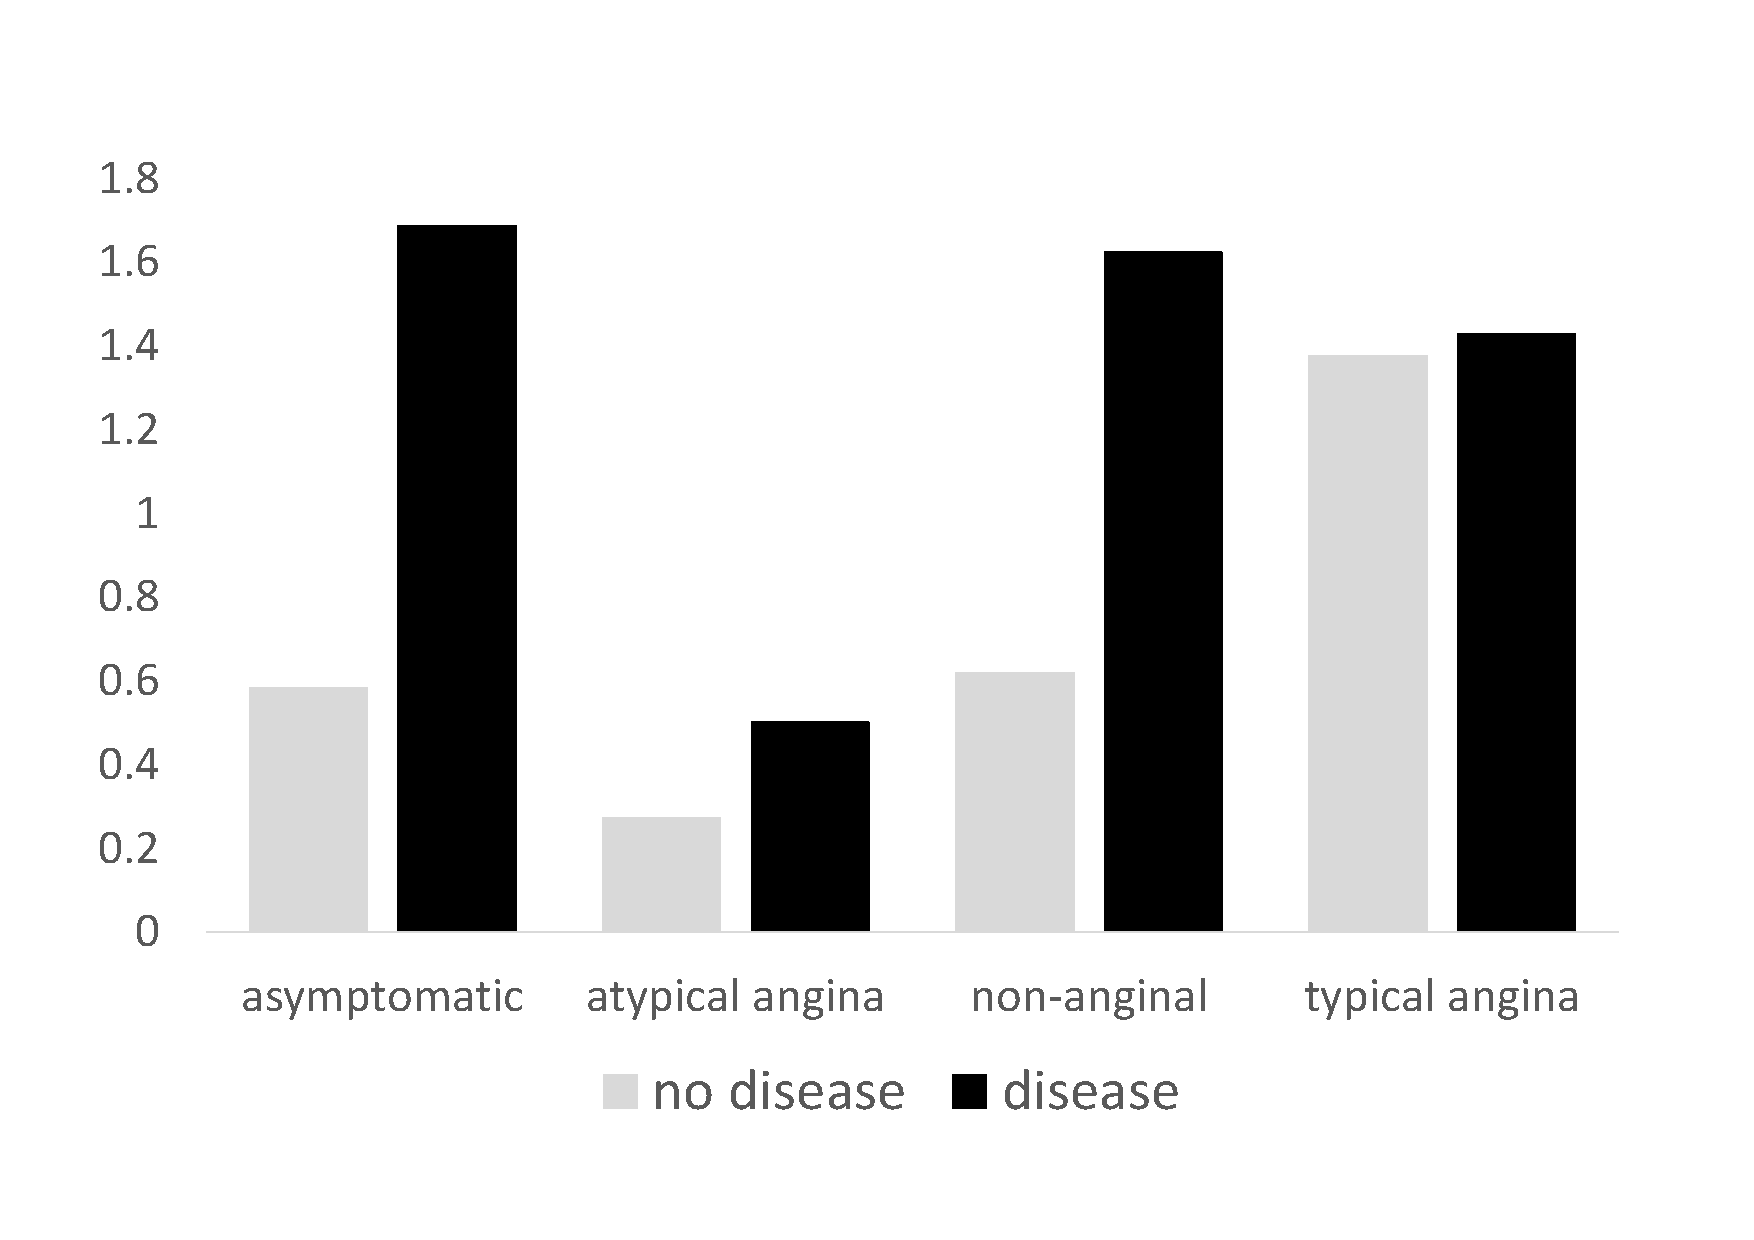
\includegraphics[width=2.7in]{figures/introduction/cp_avg_oldpeak}
	\vspace{-8pt}
	\caption{{\tt AVG}(oldpeak) vs. chest pain types}
	\label{fig:intro1}
	\vspace{-8pt}
\end{figure}

% Example /Case %


For instance, consider a data analyst trying to gain some insights into the {\em Cleveland heart disease} dataset\footnote{http://archive.ics.uci.edu/ml/datasets/heart+Disease}. 
%
Naturally, a first step in that exploratory analysis is to conduct some comparison between patients with heart disease and those without heart disease.
%
Hence, the analyst writes an SQL query that selects patients with heart disease (i.e., {\tt disease}) as the target data subset for analysis, and the remaining patients are selected as the reference data subset (i.e., {\tt no-disease}).

Since the analyzed data contains different dimensions (e.g., chest pain types, sex, etc.) and different measures (oldpeak, age, etc.), it is a challenging task for the analyst to manually select the combinations of dimensions and measures that reveal interesting insights.
%
Hence, to automatically recommend interesting bar chart visualizations, different SQL aggregate functions are applied on the views generated from all possible pairwise combinations of dimensions and measures, then the most {\em important} views are presented to the analyst.
%
For this example, Figure \ref{fig:intro1} shows the top-1 recommended view according to the deviation-based metric \cite{Vartak2015, Vartak2014}. 
%
The figure shows that an aggregate view (i.e., bar chart) based on {\it average oldpeak} (i.e.,  pressure of the ST segment, where ST segment is an isoelectric section of the ECG) vs. {\it chest pain types} exhibits a large deviation between the target view ({\tt disease}) and reference view ({\tt no-disease}). 
%
That is, patients with heart disease often suffer more from asymptomatic and non-angina chest pains, in comparison to those without heart disease.  

\begin{figure}
	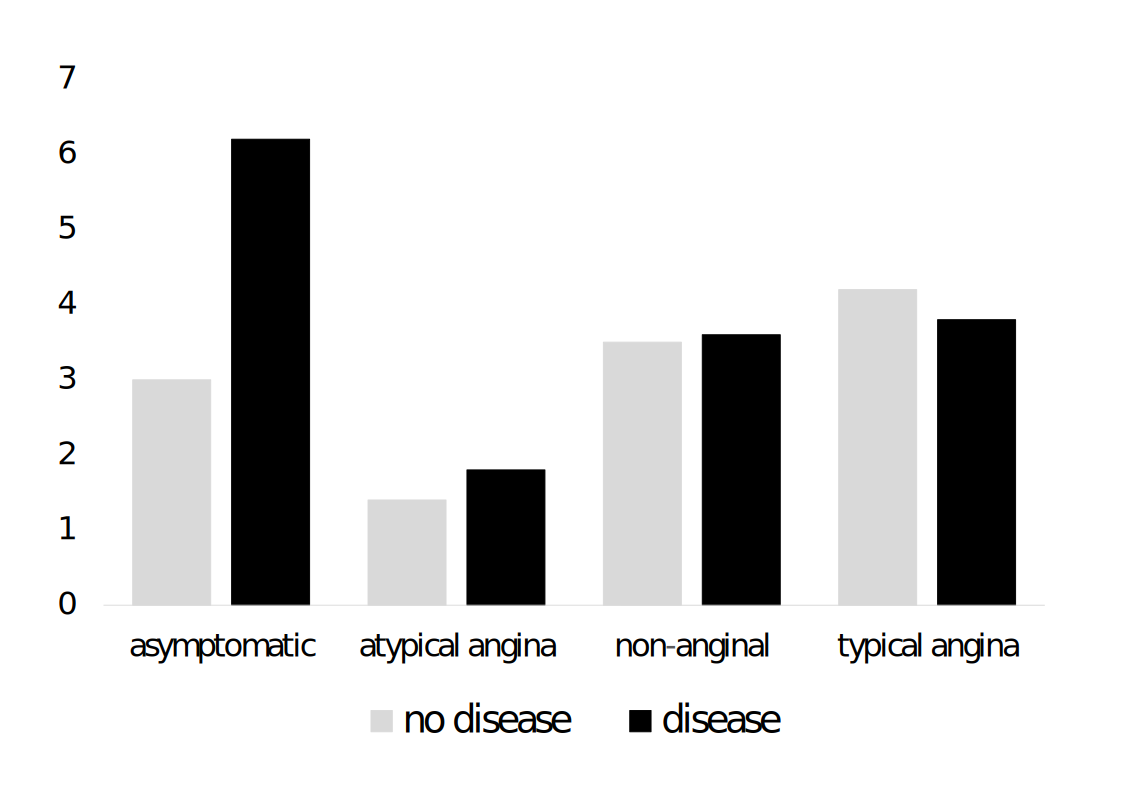
\includegraphics[width=2.7in]{figures/introduction/cp_max_oldpeak}
		\vspace{-8pt}

	\caption{ {\tt MAX}(oldpeak) vs. chest pain types}
	\label{fig:intro3}
	\vspace{-8pt}

\end{figure}

% Problem/Issue in the current solution %

While recommending views based on their importance has been shown to reveal some interesting insights \cite{Vartak2015, Vartak2014, Ehsan2016}, such approach still suffers from  a ``tunnel vision'', where it often recommends similar and redundant views. 
%
For instance, Figure \ref{fig:intro3} shows the second top recommended view for the analysis described above. 
%
Comparing Figures~\ref{fig:intro3} and \ref{fig:intro1}, it is easy to see that both views are based on the same dimension (i.e., {\it chest pain types}) and the same measure (i.e., {\it oldpeak}), and the only difference between them is the aggregate function (i.e., {\tt MAX} vs {\tt AVG}). 
%
Despite that similarity between the two views, they are still both recommended to the analyst due to the high deviation between target and reference views.


% Proposing Solution %

To address that limitation, in this work we posit that employing {\em diversification} techniques in the process of view recommendation allows eliminating that redundancy and provides full coverage of the possible insights to be discovered. 
%
In fact, diversity is rapidly becoming one of the fundamental features for maximizing information gain in web search and recommendation engines (e.g., \cite{Zhang2008,Clarke2008,Rafiei2010, Yu2009}). 
%
Similarly, it is highly desirable to recommend views that reveal interesting insights, while at the same time provide the analyst with a broad scope of those insights.

To that end, we propose a hybrid objective utility function, which captures both the importance (i.e., a deviation-based metric), as well as the diversity of insights revealed by the recommended views.
%
The main goal is to select and recommend top-k views that balance the tradeoff between importance and diversity based on the hybrid objective function. 
%

In principle, traditional data diversification methods that consider both relevance and diversity can be directly applied in the context of our problem to maximize the overall objective function (e.g., \cite{Zhang2008,Rafiei2010,Yu2009}).
%
%For instance, in the context of web search, such methods are designed to recommend a set of diversified objects (e.g., web documents) that are relevant to the user needs. 
%
However, differently from assessing  relevance, evaluating the importance of a view is a computationally expensive operation, which requires the execution of rather data-intensive queries. 
%
As such, directly applying those methods leads to a ``process-first-diversify-next'' approach \cite{Khan2015}, in which all possible data visualizations are generated first via executing a large number of aggregate queries. 
%
To address that challenge and minimize the incurred query processing cost, we propose an integrated scheme called {\em DiVE}, which leverages the properties of both the importance and diversity to prune a large number of low-utility views without compromising the quality of recommendations. 
%
The main contributions of this paper are summarized as follows: 
\begin{itemize}
	\item We formulate the problem of recommending views that are both important and diverse based on a hybrid objective function, which balances the tradeoff between the {\em content} and the {\em context} of recommended view ({\bf Section~\ref{sec:diversifying_recommended_visualizations}}). 
		
	\item We propose the novel \textit{DiVE} schemes, which employ several algorithms to select the recommended visualizations based on our hybrid ranking/objective function ({\bf Section~\ref{sec:dive_schemes}}).
	
	\item We propose novel optimization techniques that leverage the salient characteristics of our objective function to minimize the query processing cost incurred in view recommendation while maximizing the quality of recommendation ({\bf Section~\ref{sec:pruning}}).
	
	\item We conduct an extensive experimental evaluation on real datasets, which compare the performance of various algorithms and illustrate the benefits achieved by \textit{DiVE} ({\bf Sections~\ref{sec:experimental_testbed}}). 
\end{itemize}


























%
%}
%
%\eat{
%	+++ remove the figure with age and for the remaining two figures put a label on the x and y axis
%	
%	For instance, consider a Cleveland heart disease dataset \footnote{http://archive.ics.uci.edu/ml/datasets/heart+Disease}, which describes patients with and without a heart disease.  A data analyst might be interested in conducting some comparison between people with heart disease ({\bf disease}) and people without heart disease ({\bf no disease}). 
%	% Explanation of the example %
%	Let the target subset be the data of people with heart disease and the reference subset be the data of people without heart disease. As shown in Figure \ref{fig:intro1} {\it average oldpeak} (pressure of the ST segment) vs. {\it chest pain types} is more important view rather than Figure \ref{fig:intro2} the {\it average of age} vs. {\it chest pain types}, due to the large deviation between target view (disease) and reference view (no disease). 
%	%Figure \ref{fig:intro1} shows people with heart disease, especially who the chest pain types is asymptomatic tend to have much higher oldpeak rather than people without disease. 
%	To the contrary, Figure \ref{fig:intro2} is potentially less important view compared to Figure \ref{fig:intro1}, even there is a deviation but the deviation is very small and it is lower than Figure \ref{fig:intro1}. 
%	%Figure \ref{fig:intro2} shows that there is no significant different in term of the average age of the people with four types of chest pain.
%}

%\begin{figure}
%	\centering
%	\begin{subfigure}[b]{0.40\textwidth}
%		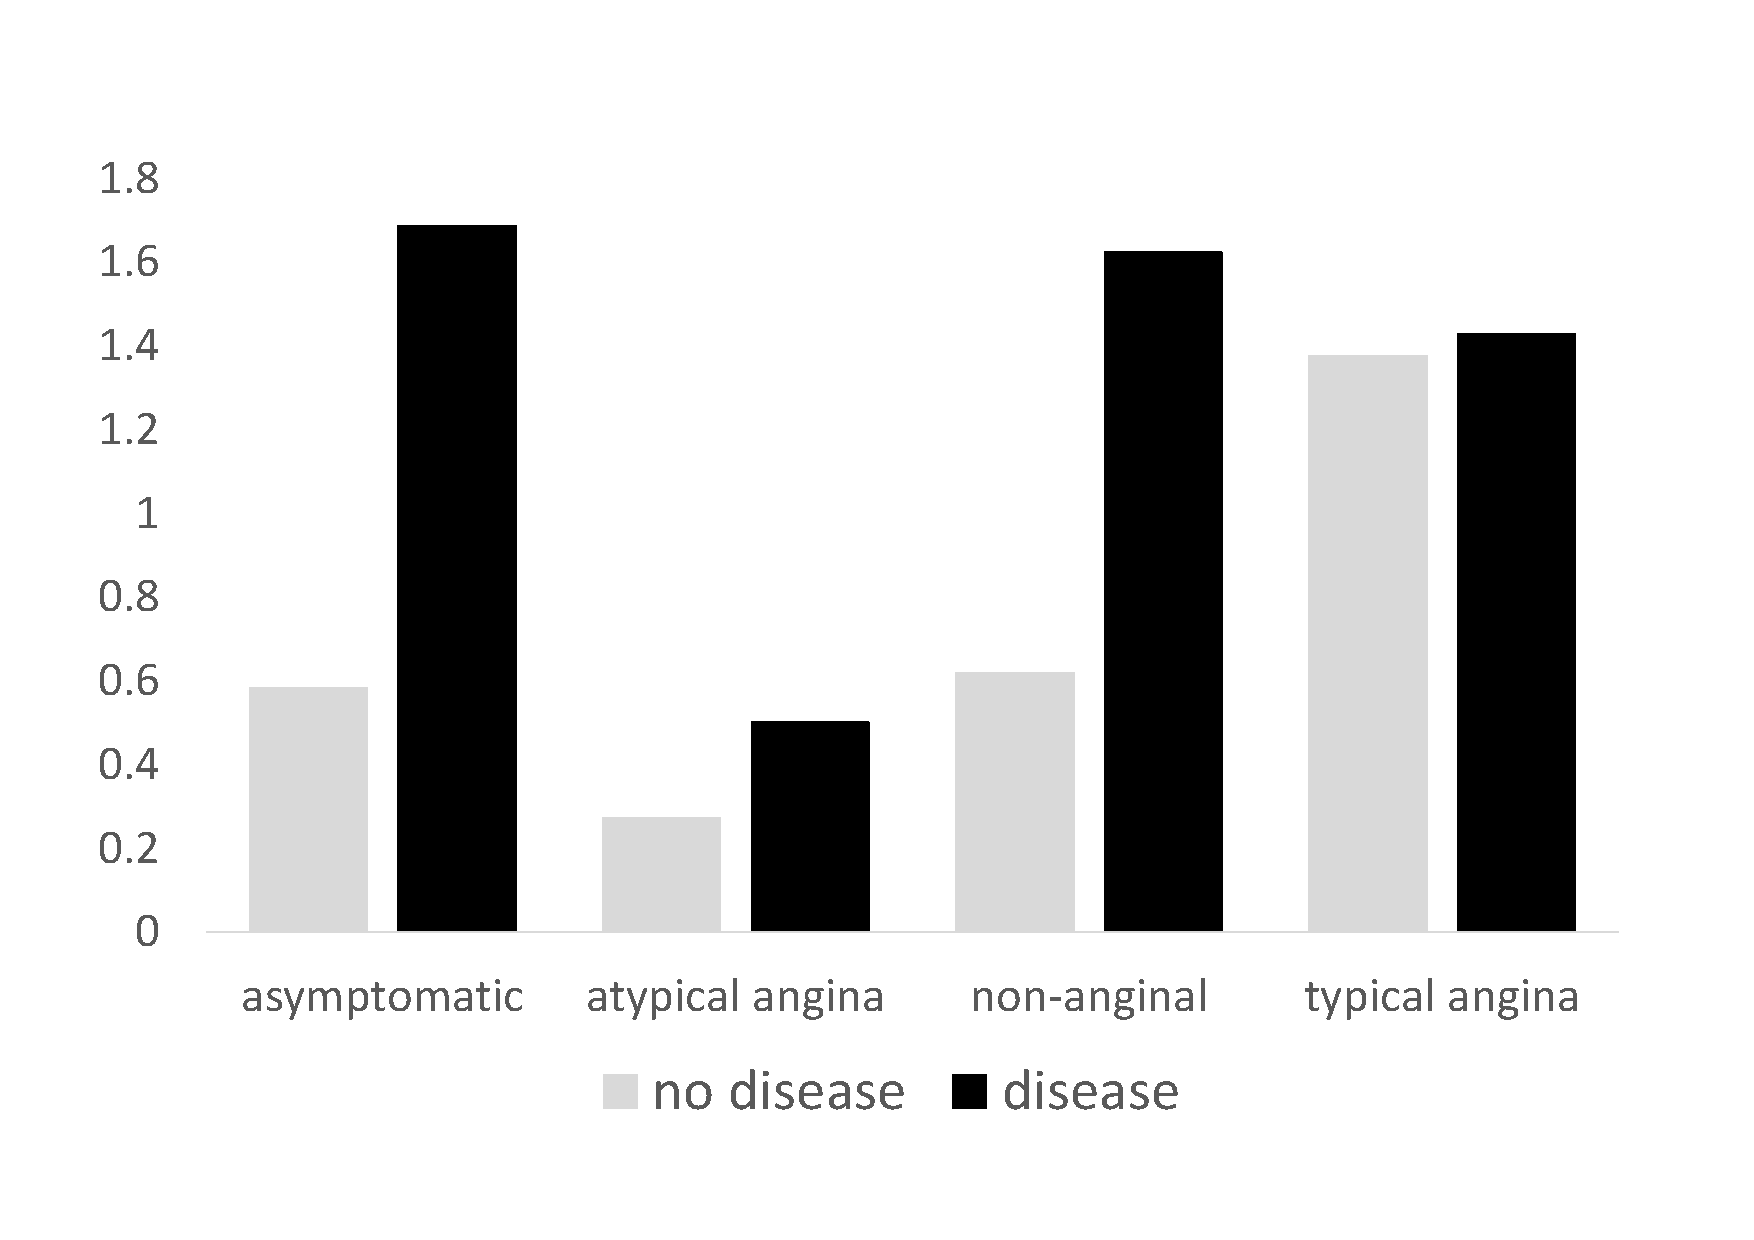
\includegraphics[width=2.5in]{figures/introduction/cp_avg_oldpeak}
%		\caption{Visualization of the avg. oldpeak vs. chest pain types}
%		\label{fig:intro1} 
%	\end{subfigure}
%	
%	\begin{subfigure}[b]{0.40\textwidth}
%		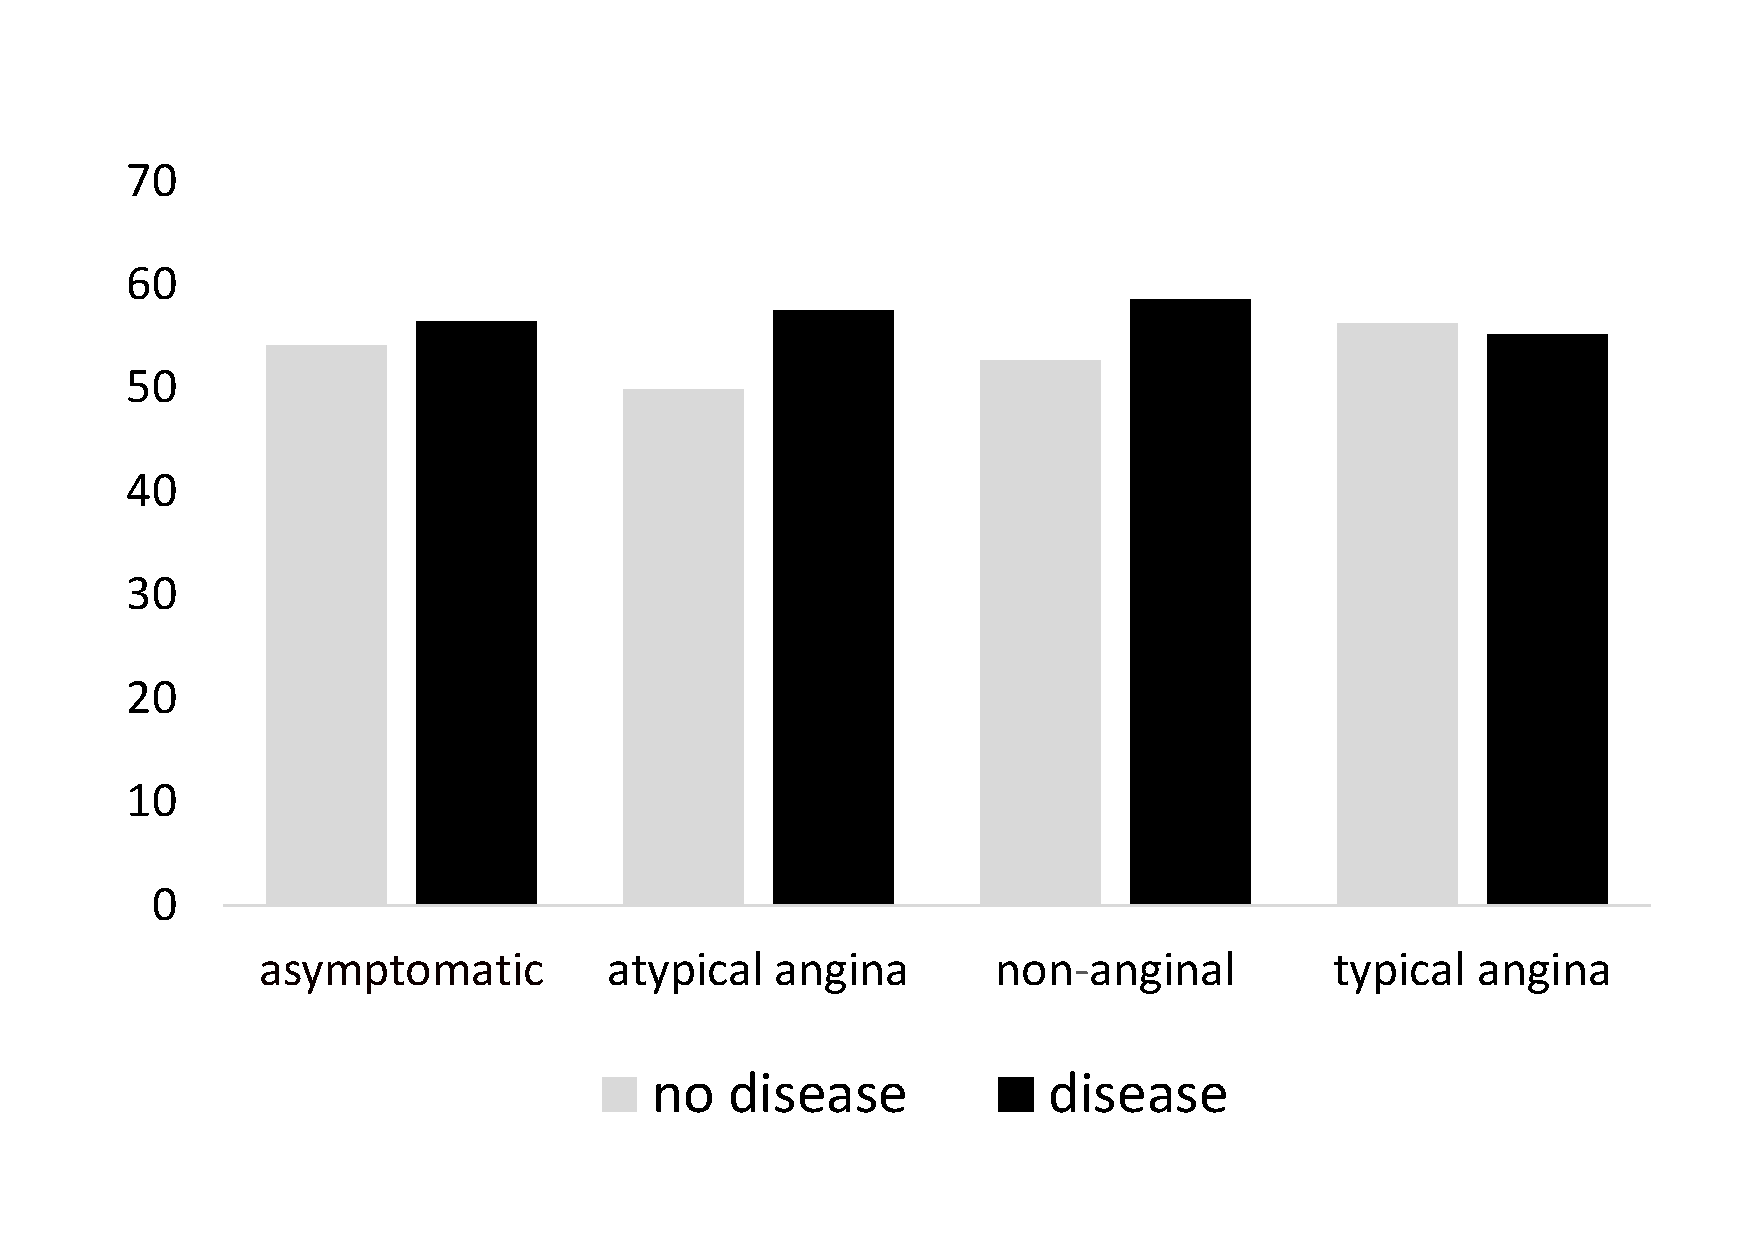
\includegraphics[width=2.5in]{figures/introduction/age_oldpeak}
%		\caption{Visualization of the average age vs. chest pain types }
%		\label{fig:intro2}
%	\end{subfigure}
%	\caption[important vs not]{Important vs. less important view.}
%\end{figure}

%In the recent years with an exponential growth of available data in various domains, there has been an increase in the number of people who trying to gain insights from the data by visual analysis ({\it data analyst}). Generaly, without any prior knowledge about the data, analyst must manually specify different combinations of attributes, measures and aggregate functions before finally generating a visualization that reveals some insights from the dataset. However, manually looking for insights in each visualization is a labor-intensive and time-consuming process. 
%
%Such challenge motivated multiple research efforts that focused on automatic recommendation of visualizations based on some metrics that capture the utility of a recommended visualizations (e.g., \cite{Key2012,Viegas2007,DBLP:journals/pvldb/SellamK16,DBLP:conf/ssdbm/SellamK16, Vartak2014,Vartak2015,Ehsan2016,kandel2012profiler,DBLP:journals/tvcg/SeoS06}. 
%
%Recent case studies have shown that {\it "a deviation-based metric"} to be effective in providing the most important visualization \cite{Vartak2014, Vartak2015}. The main goal of those works is to provide the most important visualizations ({\it top-k views}) to the analyst. In such solutions, a large number of possible views are generated and ranked according to that metric. This metric determines the deviation between the queried subset of data ({\it target view}) to the reference subset of data ({\it reference view}). The intuition behind deviation-based approach is that views that reveal substantially different trends from the reference view is judged as the important view.  

%Although the deviation-based visualization recommendation automatically provide the top-k most important views, however, it often recommends similar views and leaving the analyst with a limited amount of gained insights. 
%%
%For instance, Figure \ref{fig:intro3} provides similar insights to Figure \ref{fig:intro1}, both figures show that people with heart disease tend to have higher oldpeak values. 
%%
%Figure \ref{fig:intro3} is generated using  {\it chest pain types} as the attribute, {\it oldpeak} as the measure and {\tt MAX} as the aggregate function, whereas Figure \ref{fig:intro1}, uses same attribute and measure but uses {\tt AVG} as the aggregate function.
%%
%As shown in both figures, since those two views have a high deviation from the reference view, both views are considered as the important views and those will appear in the top-k set. 
%%
%This leads to an important observation that using "only importance" as the only criterion (e.g. a deviation-based metric) is that often deliver redundant recommended views, which leads to presents limited insights of results. 

%To address that limitation, in this work we posit that employing diversification techniques in the process of view recommendation allows eliminating that redundancy and provides concise coverage of the possible insights to be discovered. 
%%
%In fact, novelty and diversity are one of the fundamental characteristics of any effective recommendation systems \cite{Zhang2008,Clarke2008,Rafiei2010, Yu2009}. 
%%
%Specifically, it is highly desirable that a view recommendation can recommend the top-k views that are both importance and also provide new insights that has not been revealed by the other views. 

%% Lists of contributions %
%Towards designing an effective view recommendation that promotes both importance and diversity in recommended views, in this work, we propose an integrated approach called \textit{DiVE}. In particular, DiVE aims to generate top-k views that balance the tradeoff between importance and diversity. The main contributions of this paper are summarized as follows:
%
%\begin{itemize}
%	\item We formulate the problem of evaluating recommended views that are both importance and diverse ({\bf Section \ref{sec:diversifying_recommended_visualizations} }). 
%	\item We define a similarity measure to capture the distance between two visualizations ({\bf Section \ref{sec:diversifying_recommended_visualizations}}).
%	\item We present a hybrid objective function to balance the tradeoff between importance and diversity when ranking the visualizations ({\bf Section \ref{sec:diversifying_recommended_visualizations}}).
%	\item We propose the novel \textit{DiVE} schemes, that employs various algorithms to evaluate the recommended visualizations based on the hybrid ranking/objective function ({\bf Section \ref{sec:dive_schemes}}).
%	\item We present optimization techniques that leverage the hybrid objective function to substantially reduce the computational costs ({\bf Section \ref{sec:dive_schemes}}).
%	\item We conduct an extensive experimental evaluation on real datasets, which compare the performance of various algorithms and illustrate the benefits achieved by \textit{DiVE} both in terms of effectiveness and efficiency ({\bf Section \ref{sec:experimental_testbed}}). 
%\end{itemize}
\vspace{-3pt}
% Preliminaries and Related Work
% ============================================== %
% PRELIMINARIES %
% ============================================== %

%\note{general notes:
%
%1-use label{} to give each section and subsection a reference - important for roadmap and referring to sections.
%
%2-For equations, no skips, no newlines and it should be one pair of \$ for each equation - some has \$ for each symbol, makes it hard to edit 
%
%3-add all missing references and follow the standard short format
%}

\section{PRELIMINARIES AND RELATED WORK}\label{sec:preliminaries_related_work}

%\mas{preamble} 

%\subsection{Recommendation of Aggregate Views}

% Visualization Recommendation System explanation %
Several recent research efforts have been directed to the challenging task of recommending aggregate views that reveal interesting data-driven insights (e.g., \cite{Vartak2014,Vartak2015,Ehsan2016}).
%
As in previous work, we assume a similar model, in which a visual data exploration session starts with an analyst submitting a query $Q$ on a multi-dimensional database $D_B$.
%
Essentially, $Q$ selects a subset $D_Q$ from $D_B$ by specifying a query predicate $T$.
%
Hence, $Q$ is  defined as:
%
{\tt $Q$: SELECT * FROM $D_B$ WHERE $T$;}



Ideally, the analysts would like to generate some aggregate views (e.g., bar charts or scatter plots) that unearth some valuable insights from the selected data subset $D_Q$. 
%
However, achieving that goal is only possible if the analyst knows exactly what to look for!  
%
That is, if they know the parameters, which specify some aggregate views that lead to those valuable insights (e.g., aggregate functions, grouping attributes, etc.). 
%
%Meanwhile, such parameters only become clear in ``hindsight'' after spending long time exploring the underlying database.
%
Hence, the goal of existing work, such as \cite{Viegas2007,Key2012,Vartak2014,Vartak2015,Ehsan2016}, is to {\em automatically} recommend such aggregate views. 
%

To specify and recommend such views, as in previous work, we consider a multi-dimensional database $D_B$, which consists of a set of dimensional attributes $\mathbb{A}$ and a set of measure attributes $\mathbb{M}$. 
%
Also, let $\mathbb{F}$ be a set of possible aggregate functions over measure attributes. %, such as {\tt COUNT, AVG, SUM, MIN and MAX}. 
%
Hence, specifying different combinations of dimension and measure attributes along with various aggregate functions, generates a set of possible views $\mathbb{V}$ over the selected dataset $D_Q$.
%
For instance, a possible aggregate view $V_i$ is specified by a tuple <$ A_i$, $ M_i$, $ F_i$>, where $A_i \in \mathbb{A}$, $M_i \in \mathbb{M}$, and  $F_i \in \mathbb{F}$, and it can be formally defined as:
%
{\tt $V_i$: SELECT $A_i$, $F_i$ ($M_i$) FROM $D_B$ WHERE $T$ GROUP BY $A_i$};



%Clearly, an analyst would be interested in those views that reveal interesting insights. 
%
Manually looking for insights in each view $V_i \in \mathbb{V}$ is a labor-intensive and time-consuming process. 
%
%For instance, consider again our example in the previous section. 
%
%In that example, let $D_B$ be the Cleveland Heart Disease table (i.e., {\tt tb\_heart\_disease}) and the analyst is selecting the subset of patients with heart disease (i.e., {\tt $D_Q$ = disease} subset).
%
Particularly, the number of views to explore is equal to: $|\mathbb{V}|$ = $|\mathbb{A}| \times |\mathbb{M}| \times |\mathbb{F}|$, where $|\mathbb{F}|$ is the number of SQL aggregate functions, and $|\mathbb{A}|$ and $|\mathbb{M}|$ are the number of attribute and measures. %in {\tt tb\_heart\_disease}, respectively. 
%
%For that medium-dimensionality dataset, that value of $|\mathbb{V}|$ goes up to $180$ views, which is clearly unfeasible for manual exploration. 
%
Such challenge motivated multiple research efforts that focused on automatic recommendation of views based on some metrics that capture the utility of a recommended view (e.g., \cite{Key2012,Viegas2007,DBLP:journals/pvldb/SellamK16,DBLP:conf/ssdbm/SellamK16, Vartak2014,Vartak2015,Ehsan2016,kandel2012profiler,DBLP:journals/tvcg/SeoS06}). 
%
%\mas{next sentences need to be more specific - one sentence for each of those works! The point is to show there is a space of recommendation methods and we are selecting the deviation-based one. Can come from your old related work section or from Humaira's TKDE}

Those approaches can be broadly classified as {\em user-driven} or {\em data-driven}.
%
User-driven solutions focus on recommending visualizations that facilitate a particular user intent or task. 
%
For example, VizDeck \cite{Key2012} utilizes user feedback as a basis for view recommendation, whereas Profiler \cite{kandel2012profiler} detects anomalies and recommends visualizations based on mutual information metric.
%
Similarly, Rank-by-Feature Framework \cite{DBLP:journals/tvcg/SeoS06} enables users to select their criterion for ranking histograms and scatter-plots. 
%

Meanwhile, {\em data-driven} focus on enabling the discovery of interesting insights from large volumes of data without requiring much prior knowledge of the explored data.
%
Towards that end, data-driven metrics are employed to capture the {\em interestingness} or {\em importance} of a recommended visualization. 
%
Recent case studies have shown that a {\em deviation-based} metric is effective in providing analysts with {\em important} visualizations that highlight some of the particular trends of the analyzed datasets \cite{Vartak2015, Vartak2014, TKDEHumaira, Ehsan2016}.

%++ site humaira
%
%++ remove table and any reference to it

%
In particular, the deviation-based metric measures the distance between $V_i(D_Q)$ and $V_i(D_R)$. 
%
That is, it measures the deviation between the aggregate view $V_i$ generated from the subset data $D_Q$ vs. that generated from a reference dataset $D_R$, where $V_i(D_Q)$ is denoted as {\em target} view, whereas $V_i(D_R)$ is denoted as {\em reference} view. 
%
That reference dataset could be the whole database (i.e., $D_R=D_B$) or a selected subset of the database (e.g., Sec. ~\ref{introduction}). 
%
%
The premise underlying the deviation-based metric is that a view $V_i$ that results in a high deviation is expected to reveal some important insights that are very particular to the subset $D_Q$ and distinguish it from the patterns in $D_R$.
%
In case, $D_R=D_B$, then the patterns extracted from $D_Q$ are fundamentally different from the generals ones manifested in the entire database $D_B$.  

While recommending views based on their importance has been shown to reveal some interesting insight, it also suffers from the drawback of recommending similar and redundant views, which leaves the data analyst with a limited scope of the possible insights.    
%%
%\mas{refer back to the intro example and reiterate that issue in one sentence}
As illustrated in the previous section, Figures~\ref{fig:intro1} and~\ref{fig:intro3} show two recommended views that basically reveal the same insight.  
%
To address that limitation, in this work we posit that employing {\em diversification} techniques in the process of view recommendation allows eliminating that redundancy and provides a good and concise coverage of the possible insights to be discovered.
%%
In the next section, we discuss in details the formulation of both importance and diversity, and their impact on the view recommendation process.
%


%\note{check table-text consistency and make shorter - done}
%\note{also noticed that many symbols are often mentioned in the text without \$ especially $K$ and $S$}
\eat{
\begin{table}
	\caption{Table of Symbols}
	\label{tab:tab-symbols}
	\begin{tabular}{ccl}
		\toprule
		Symbol &Description\\
		\midrule
		k & no. of top recommended views\\
		S & set of top-k recommended views\\
		%S* & optimum set of views \\
		$ \mathbb{V}  $& set of all possible views\\
		X & set of all candidate views\\
		$ A $ & a dimensional attribute \\%/ member of set of attributes $ \mathbb{A} $\\
		$ M  $& a measure attribute\\ %/ member of set of meassures $ \mathbb{M} $\\
		$ F $ & aggregate function \\%/ member of set of agg. funcs. $ \mathbb{F} $\\
		$ Q $ & a user query \\
		$ D_B  $& a multi-dimensional database \\
		$ D_Q  $& a target subset of $ D_B  $\\
		$ D_R  $& a reference subset of $ D_B  $\\\
		$ V_i  $& a view query\\
		$ I$($V_i$)  & importance score of $ V_i $\\
		$ I$($S$)  & importance score of views in S\\
		%$ Ctx(V_i)  $& the context of $V_i$\\
	%	$ D $  & the contextual distance measure\\ %between two views\\
		$ f$($S$,$D$) & diversity score of views in S\\
		$ F$($S$)  &  hybrid objective utility function value of S \\
		$ U$($V_i$) &  the utility score of each candidate view \\
		%$ max_I$ &  the maximum value of importance\\
		\bottomrule
	\end{tabular}
\end{table}
}
\vspace{-3pt}
% ============================================== %
% PRELIMINARIES %
% ============================================== %

\begin{figure*}
	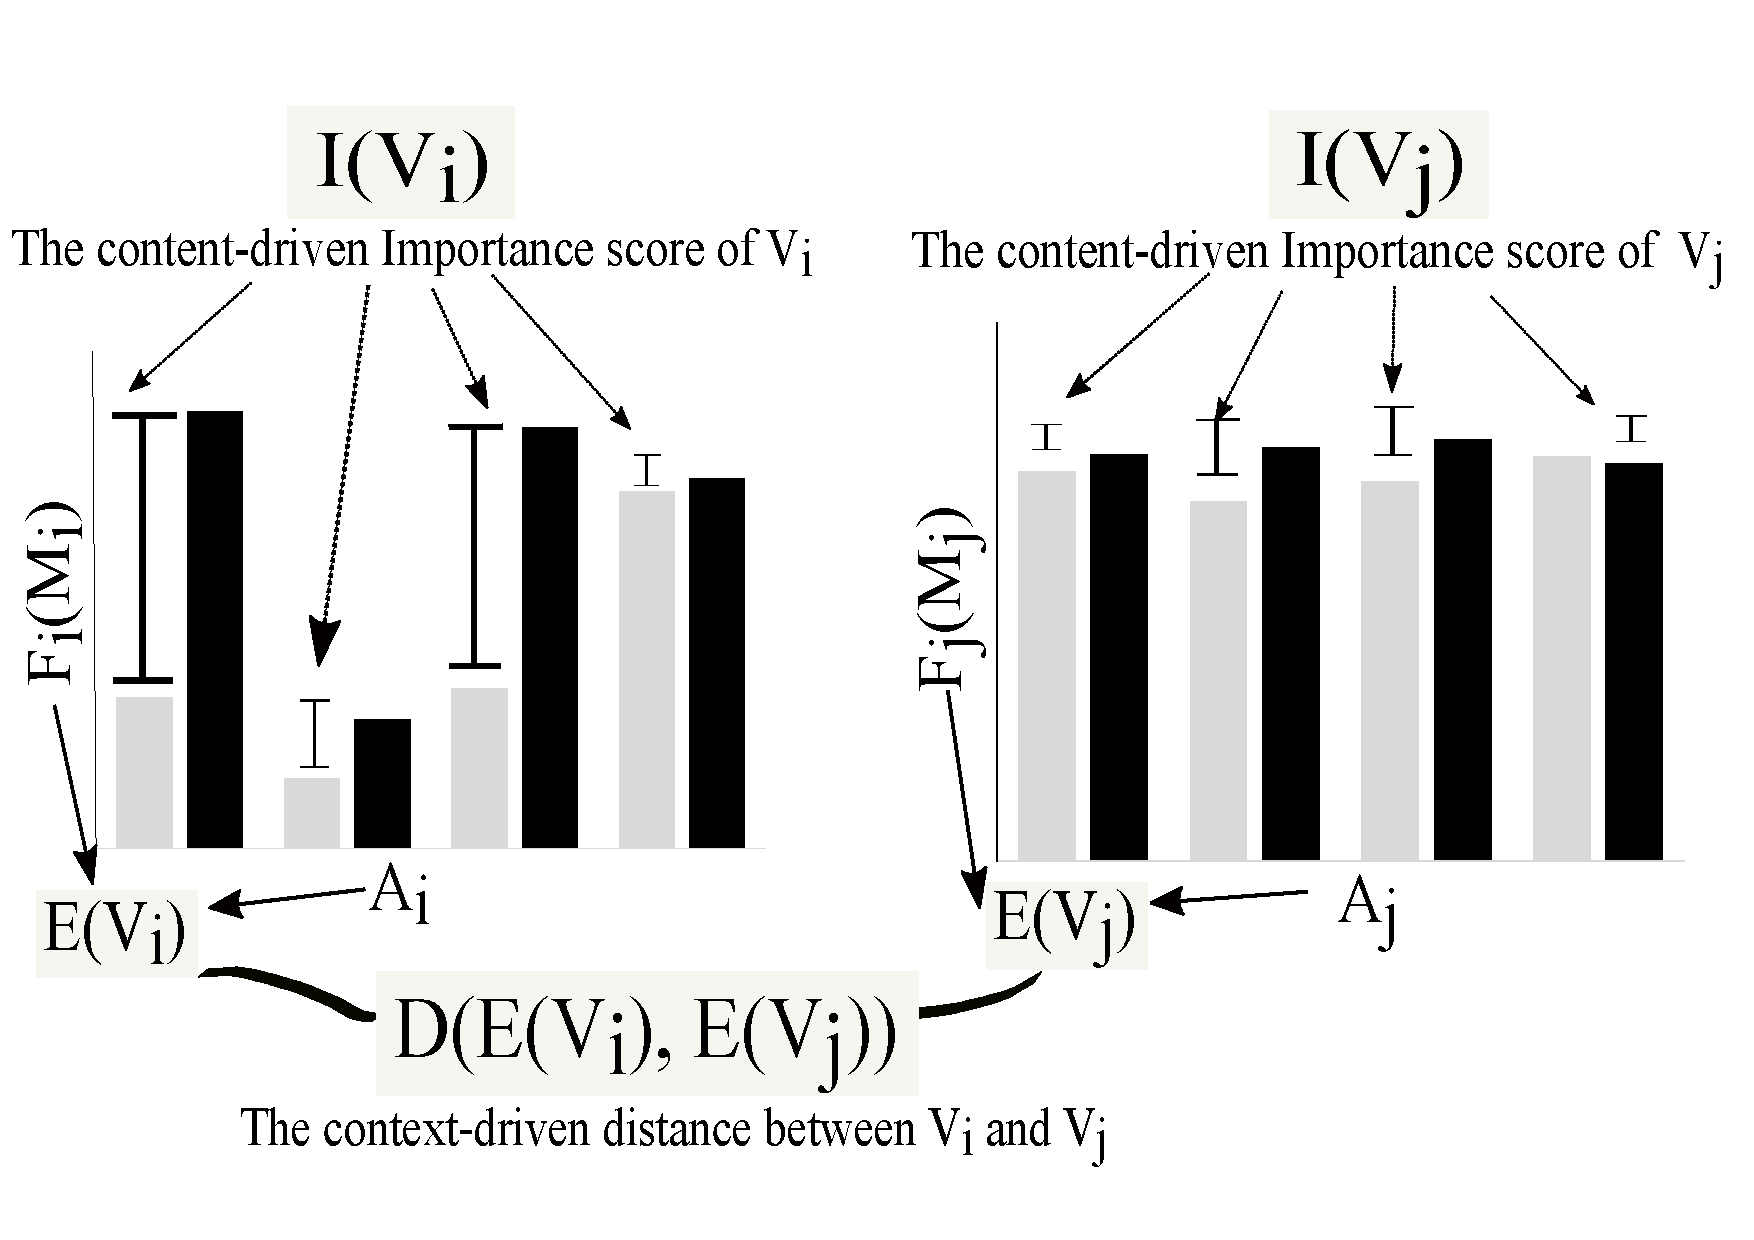
\includegraphics[width=6in,height=3in]{figures/introduction/pre2}
	\vspace{-12pt}
	\caption[content vs context]{Content vs. Context of views.}
	\label{fig:content-contex}
	%\vspace{-12pt}
\end{figure*}


\section{Diversifying Recommended Views}
\label{sec:diversifying_recommended_visualizations}
% %

%\mas{short preamble}

Towards formulating our hybrid objective for view recommendation, in this section we describe the {\em content-based} deviation metric for assessing the importance of each view (Sec.~\ref{subsec:content_driven_deviation}), together with our {\em context-based} measure of the (dis)similarity between different views (Sec.~\ref{context-driven-deviation}). 
%
Those two metrics provide the foundations for our hybrid objective that aims to balance the tradeoff between importance and diversity in view recommendation (Sec.~\ref{subsec:problem_definition}).  
\vspace{-8pt}

\eat{
In order to diversifying recommended visualizations, we work at two levels. At the first level, content driven deviation metric is used to evaluate that how \quotes{important} is the content of the view as compared to the reference view. At the second level, we evaluate contextually how different a view is from other views in the recommended set using context driven deviation measure. The details of those two level are described next. 
}

\subsection{Content-Driven Importance}
\label{subsec:content_driven_deviation}

As  described in the previous section, we adopt a deviation-based metric to quantify the importance of a view \cite{Vartak2015,Vartak2014}. 
%
Essentially, the deviation-based metric compares an aggregate view generated from the selected subset dataset $D_Q$ (i.e., target view $V_i(D_Q)$) to the same view if generated from a reference dataset $D_R$ (i.e., reference view $V_i(D_R)$). 
%
%That reference dataset could be the whole database (i.e., $D_R=D_B$) or a selected subset of the database. 
%

Clearly, the deviation between a target and a reference view is a {\em data-driven} metric. 
%
That is, it measures the deviation between the {\em result} of $V_i(D_Q)$ and that of $V_i(D_R)$. 
%
Consequently, from a visualization point of view, that deviation is a {\em content-based} metric that captures the difference between the content of the visualization generated by $V_i(D_Q)$ vs. the visual content of  $V_i(D_R)$.
%
In the next, we formally describe the standard computation of that data-driven content-based metric, whereas the discussion of its counterpart context-driven metric is deferred to the next section.

To calculate the content-based deviation, each target view $V_i(D_Q)$ is normalized into a {\em probability distribution} $P[V_i(D_Q)]$ and similarly, each reference view into $P[V_i(D_R)]$.
%
In particular, consider an aggregate view $V_i=<\!A_i,M_i,F_i\!>$. 
%
The result of that view can be represented as the set of tuples: $<\!(a_j, g_j), (a_j, g_j), ..., (a_t, g_t)\!>$, where $t$ is the number of distinct values (i.e., groups) in attribute $A_i$, $a_j$ is the $j$-th group in attribute $A_i$, and $g_j$ is the aggregated value $F_i(M_i)$ for the group $a_j$ \cite{Ehsan2016, Vartak2015}. 
%
Hence, $V$ is normalized by the sum of aggregate values $G=\sum\limits_{j=1}^{t} g_j$, resulting in the probability distribution $P[V_i] = <\!\frac{g_1}{G}, \frac{g_2}{G}, ..., \frac{g_t}{G}\!>$.
%

Finally, the importance score of $V_i$ is measured in terms of the distance between $P[V_i(D_Q)]$ and $P[V_i(D_R)]$ (as illustrated in Figure~\ref{fig:content-contex}), and is simply defined as:
\begin{equation}
	I\left(V_i\right) = dist\left(P\left[V_i(D_Q)\right], P\left[V_i(D_R)\right]\right)
	\label{importance_score}
\end{equation}

\noindent where $ I\left(V_i\right) $ is the importance score of $ V_i$ and \textit{dist} is a distance function. 
%
Similar to existing work (e.g., \cite{Vartak2014,Vartak2015}), we adopt a Euclidian distance, but other distance measures are also applicable (e.g., Earth Mover's distance, K-L divergence, etc.). 

In current approaches for view recommendation, the importance value $I(V_i)$ of each possible view $V_i$ is computed, and the $k$ views with the highest deviation are recommended.
%
However, in this work, our goal is to ensure that recommended views provide a good coverage of possible insights, which is described next. 
\vspace{-2pt}
\subsection{Context-Driven Similarity}
\label{context-driven-deviation}
% % Prolog 

As mentioned above, recommending views based only on their data content often leads to a set of similar views. 
%
In order to provide full coverage of all possible interesting insights, in this work, we posit that achieving {\em diversity} within the set of recommended views is an essential quality measure. 
%
%Diversity has been well known and widely used in recommendation systems for maximizing information gain and minimizing redundancy (e.g., \cite{Zhang2008, Rafiei2010, Yu2009, Vieira2011}). 
%
%At a high level, diversity essentially measures how different (i.e., diverse) are the individual data objects within a set. 
%	
Before discussing the details of diversity computation in Sec.~\ref{subsec:problem_definition}, it is important to notice that central to that computation is some notion of distance measure between data objects.
%
Existing work provides multiple metrics for measuring that distance between traditional data objects, such as web documents (e.g., \cite{Rafiei2010,Clarke2008,Zhang2008}), database tuples (e,g, \cite{DBLP:conf/sigmod/TranC10}), etc.
%
However, our work in this paper is the first to consider diversity in the context of aggregate data visualizations. 
%
As such, a metric is needed to quantify the (dis)similarity between the distinct features of different visualizations.
%
Towards this, we re-emphasize that each visualization is merely a data view generated by an aggregate query. 
%
Thus, such metric naturally lends itself to considering the query underlying each view (i.e., the query  executed to create the view). 
%
In turn, the distance between two views is measured based on the distance between their underlying queries.  
%
Hence, in addition to our data-driven content-based deviation, we also introduce a query-driven {\em context-based} deviation metric.
%
 Figure~\ref{fig:content-contex} illustrates and summarizes our proposed metrics.
	


%To measure the context-based deviation between two visualizations, we simply measure the distance between their underlying queries. 
%
Towards measuring the context-based deviation, we extend on existing work in the area of query recommendation and refinement (e.g., \cite{DBLP:conf/sigmod/TranC10,DBLP:conf/dexa/Kantere16,DBLP:conf/cikm/KantereOKS15}).
%
In that work, the distance between two range queries $q_1$ and $q_2$ is mapped to that of measuring the edit distance needed to transform $q_1$ into $q_2$. %where the set of allowed transformation are: add, delete, or modify a predicate. 
%
In the context of our work, however, views are generated from aggregate queries without range predicates. 
%
In particular, a view is fully defined in terms of a combination of attribute, measure and an aggregate function.
%
Hence, in addition to the content of a view $V_i$ which is described by its probability distribution (i.e., $P(V_i))$ as defined in Sec. ~\ref{subsec:content_driven_deviation}), we also consider the context of the view $E(V_i)$, which is defined in terms of the query underlying $V_i$ as:
%
$E(V_{i})=  \{A_i, M_i, F_i\}$.




Such definition of view context leads to a special case of the existing work on query recommendation, in which the normalized distance between two queries is simply measured using the {\em Jaccard} similarity measure.
%
Hence, the Jaccard similarity between two aggregate views $V_i$ and $V_j$ is measured as: $ J(V_{i}, V_{j} ) = \dfrac{| E(V_{i}) \cap E(V_{j}) |}{| E(V_{i}) \cup E(V_{j})|} $	
%\note{update figure to reflect all those changes here and also check all equations for mistakes while making the changes}
%done

We note that the jaccard similarity assigns equal weights to each of the element in a set. 
%
Accordingly, when applied to aggregate views, then two views with the same attribute and different measure and aggregate function will have the same similarity score as any other pair of views with same measure but different attribute and aggregate function. 
%
However, an analyst may consider two views with the same attribute $A_i$ more similar than two views with same measure attribute $M_i$. 
%
To allow the analyst to specify such preference, each contextual component of a view is associated with a weight that specifies its impact on determining the (dis)similarity between views. 
%
Specifically, let $w_i$ be the weight assigned to $i^{th}$ element of set $E(V_i)$, where $\sum_{i=1}^{3}w_i =1$.
%
Then, the similarity between views $V_i$ and $V_j$ is measured as: $J(V_{i}, V_{j} ) = \dfrac{\sum_{i\in V_i \cap V_j}w_i}{\sum_{i\in V_i \cup V_j}w_i} $
%	
Consequently, the context-based deviation between $V_i$ and $V_j$ is calculated as:
\vspace{-4pt}
\begin{equation}
D\left(V_{i}, V_{j} \right) = 1- J\left(V_{i}, V_{j} \right) 
\label{diversity_score}                 
\end{equation}
\vspace{-14pt}



%
\eat{
Particularly, it shows two views $V_i$ and $V_j$, for which the content-driven importance values $I(V_i)$ and $I(V_j)$ are computed based on the probability distribution of the data in each view. 
%
Moreover, it also shows the context-driven distance between those two views, which is computed as $D\left(V_{i}, V_{j} \right)$. 
}

\eat{
% %
As a summarize, the difference betweeen content and context of view is described in Figure \ref{fig:content-contex}.
% %
Content is the probability distribution of the aggregated query result, whereas, Context is described as a set containing the name of the attribute, measure and function used to generate the view.  
% %
		}

\eat{
Thus, in the process to recommend users a set of top-k views, we work at two levels.
% %
At the first level, we evaluate that how \quotes{important} is the content of the view as compared to the reference view using content driven deviation metric. 
%In particular, we determine how different are the trends and patterns revealed by $V_{T}$ from its reference $V_{R}$ in terms of content. 
% %
At the second level, we evaluate contextually how different a view is from other views in the recommended set using context driven deviation measure. 
% %
}


%
%
%% %
%The difference betweeen content and context is described in Figure \ref{fig:pre}.
%% %
%Content as in Figure \ref{fig:pre1} is the probability distribution of the aggregated query result, whereas, Context as in Figure \ref{fig:pre2} is described as a set containing the name of the attribute, measure and function used to generate the view.  
%
%% %

% ============================================== %
% PRELIMINARIES %
% ============================================== %

\subsection{Problem Definition}\label{subsec:problem_definition}
% %
% %
In this section, we formally define our problem for recommending diversified interesting aggregate views.  
%
Towards this, we first define the metrics to measure the performance of our proposed visualization recommendation system.

% in terms of: 1) the quality of recommended visualizations, and 2) the processing cost incurred in computing those visualizations.

\subsubsection{Hybrid Objective Function}

Our hybrid objective function is designed to consider both the importance and diversity of the recommended views. 
%
Particularly, it integrates two components: 1) the total importance score of set $S$ and 2) the diversity score of $S$.

The importance score of the a $S$ is calculated as the average value of the importance measure of each view in $S$, as given in Eq.\ref{importance_score}. 
%
Hence, the total importance score of $S$ is defined as: $ I\left(S\right)= \sum_{i=1}^{k} \dfrac{I(V_i )}{I_u}, V_i  \in S $, where $I_u$ is the upper bound on the importance score for an individual view, which is achieved when for each group $a_i$, the corresponding value $\frac{g_i}{G}$ in $P[V_{i}(D_R)]$ or $P[V_{i}(D_Q)]$ is zero. Thus, $I_u = \sqrt{2}$, and is used to normalize the average importance score for set $S$. 

In order to measure the diversity of a set of objects, several diversity functions have been employed in the literature \cite{Vieira2011, Clarke2008}. 
%
Among those, previous research has mostly focused on measuring diversity based on either the average or the minimum of the pairwise distances between the elements of a set \cite{Wu2014}. 
%
In this work, we focus on the first of those variants (i.e., average), as it maximizes the coverage of $S$. 
%
Hence, given a distance metric $ D\left(V_i, V_j\right) $, as given in equation \ref{diversity_score}, the diversity of a set $S$ can be simply measured as follows:

$ f\left(S,D\right)= \dfrac{1}{k\left(k-1\right)}  \sum_{i=1}^{k} \sum_{j>i}^{k} D\left(V_i,V_j\right) ,V_i,V_j  \in S $

Since the maximum context-based deviation between any two views in equation \ref{diversity_score}  is 1.0, then dividing the sum of distances by $k\left(k-1\right)$ ensures that the diversity score of set $S$ is normalized and bounded by 1.0.

%Next, we define our proposed hybrid objective function that captures both the importance and diversity of the set of recommended views $S$. 
%
Putting it together, for a set of views $S \subseteq V$, our hybrid objective function is formulated as the linear weighted combination of the importance score, $ I\left(S\right) $ and diversity score $ f\left(S,D\right) $, and is defined as:
\begin{equation}
F\left(S\right) =  \left(1-\lambda\right) \times I\left(S\right) + \lambda \times f\left(S,D\right)
\label{objectif_function}
\end{equation}

where $ 0 \leq \lambda \geq 1 $ is employed to control the preference given to each of the importance and diversity components. 
%
For instance, a higher value of $  \lambda $ results in a set of more diverse views, whereas a lower value of $ \lambda $ generates a set of the most important views, which is likely to exhibit redundancy in the recommended views. 
%

Given the hybrid objective function, our goal is to find an optimum set of views  $ S^* $ that maximizes the objective function $ F\left(S\right) $, which is defined as follows:
\begin{definition} 
{\bf Recommending diversified important views :} Given a target subset $D_Q$  and a reference subset $D_R$, the goal is to recommend a set $S \subseteq \mathbb{V}$, where $|S| = k$, and $\mathbb{V}$ is the set of all possible target views, such that the overall hybrid objective $ F\left(S\right) $ is maximized. 
\end{definition} 

\eat{
\begin{equation}
S^* = \underset{\underset{|S|=k} {S \subseteq \mathbb{V}}} {\mathrm{argmax}} F\left(S\right) 
\label{argmaxF}
\end{equation} 
}
%
%Given the definition above, the quality of the recommended set of views is measured in terms of the value of the hybrid objective function $F\left(S\right)$.





\vspace{-7pt}
\subsubsection{Cost of Visualization Recommendation}

Exisiting research has shown that recommending aggregate data visualizations based on data-driven content-based deviation is a computationally expensive task \cite{Vartak2014, Vartak2015, Ehsan2016}.
%
Moreover, integrating diversification to the view recommendation problem, as described above, further increases that computational cost.
%
In particular, the incurred processing cost includes the following two components: 1) Query processing cost $C_Q$: measured in terms of the time needed to execute and compare all the queries underlying the set of target views as well as their corresponding reference views (i.e., content-based deviation), and 2) View diversification cost $C_D$: measured in terms of the time needed to compute all the pairwise distances between each pair of target views (i.e., context-based deviation).
%
Consequently, the total cost $C_T$ for recommending a set of views is simply defined as: $C_T= C_Q + C_D$

In principle, traditional data diversification methods that consider both relevance and diversity can be directly applied in the context of our problem to maximize the objective function Eq.\ref{objectif_function}.
%
For instance, in the context of recommending web search, such methods are designed to recommend a set of diversified objects (e.g., web documents) that are relevant to the user needs. 
%
However, in that setting, the relevance of an object is either given or simply computed.
%
To the contrary, in our setting for view recommendation, the importance of a view is a computational expensive operation, which requires the execution of a target and reference view. 
%
As such, directly applying those methods leads to a ``process-first-diversify-next" approach, in which all possible data visualization are generated first via executing a large number of aggregate queries. 
%
To address that challenge and minimize the incurred query processing cost, next we propose our {\em DiVE} scheme, which leverages the properties of both the importance and diversity to prune a large number of low-utility views, without compromising the quality of recommendations. 

\eat{
\note{
However, in this work, we optimze the query execution time by reducing the search sapce of candidate views. Ou proposed pruning scheme leverages the properties of importance and diversity metrics to prune a large number of low-utility views. The details of the pruning scheme are presented later in the paper.
}



\note{

In this section, we formally define the problem of recommending a set of k views that are interesting as well as diverse among themselves. In particular, given a target subset $\mathcal{D_Q}$  and a reference subset $\mathcal{D_R}$ , set of all possible views $\mathbb{V}$, our objective is to select a set $S \subseteq \mathbb{V}$  where $|S|$ = k, such that the Interestingness score of the views in $S$ and their mutual diversity is maximized. 

Making visualization recommendations, particularly based on both data and context, is a computationally expensive task. Although hundreds of visualizations are possible for a given subset of data, only a small fraction of the visualizations are actually of interest and are included in the top-k set. Consequently, a significant fraction of the query processing cost is incurred on evaluating low-utility visualizations. Hence, in this work along with the quality of set $S$, we also aim to minimize the query processing cost of computing $S$. In particular, we apply effective pruning techniques to reduce the search space of visualizations. 


Next, we define the metrics to measure the performance of our proposed visualization recommendation system in terms of quality of recommended visualizations and processing cost of computing those visualizations.

\subsubsection{Hybrid Objective Function}

Our hybrid objective function is designed to consider both the importance and diversity of the recommended views. Thus, we split the objective function into two components: 1) total importance score of set $S$ and 2) the diversity score of $S$.


The importance score of the set S is calculated as the average value of the importance measure of each view in S, as given in equation \ref{importance_score}. Formally, the total importance score of S is defined as:
\newline

\centerline{$ I\left(S\right)= \dfrac{\dfrac{1}{k} \sum_{i=1}^{k} I(V_i )}{I_u}, V_i  \in S $}
\bigskip

where $I_u$ is the upper bound on the importance score for an individual view. The value of $I_u$ is used to normalize the average importance score for set S. (i dont understand why this normalization is needed.)



In order to measure the diversity of a set of objects, several diversity functions have been employed in the literature \cite{Vieira2011, Clarke2008}. Among those, previous research has mostly focused on measuring diversity based on either the average or the minimum of the pairwise distances between elements of set \cite{Wu2014}. We focus on the first of those variants (i.e., average), as it considers all the views in S. Given a distance matric $ D\left(V_i, V_j\right) $ as given in equation \ref{diversity_score}, the diversity of a set S can be measured by a diversity function $ f\left(S,D\right) $ that captures the dissimilarity between the views in S, defined as:
\newline

$ f\left(S,D\right)= \dfrac{1}{k\left(k-1\right)}  \sum_{i=1}^{k} \sum_{j>i}^{k} D\left(V_i,V_j\right) ,V_i,V_j  \in S $
\newline

The maximum contextual distance between two views as in equation \ref{diversity_score}  is 1. Therefore, dividing the sum of distances between all views in S by $k\left(k-1\right)$ ensures that the diversity score of set S is normalized.

Next, we define our proposed hybrid objective function that captures both importance and diversity of the set of recommended views S. Specifically, for a set of views S $\subseteq V$ an objective function is formulated as the linear weighted combination of the importance score, $ I\left(S\right) $ and diversity function $ f\left(S,D\right) $ which is defined as:


\begin{equation}
F\left(S\right) =  \left(1-\lambda\right).I\left(S\right) + \lambda.f\left(S,D\right)
\label{objectif_function}
\end{equation}


where $ 0 \leq \lambda \geq 1 $ is employed to control the contribution between importance and diversity in the hybrid objective function. The higher values of $  \lambda $ result in a set of more diverse views whereas lower values of $ \lambda $ generate a set of the most important views that might be similar to each other. 
Given the hybrid objective function, our goal is to find an optimum set of views  $ S^* $ that maximizes the objective function $ F\left(S\right) $: 

\begin{equation}
S^* = \underset{\underset{|S|=k} {S \subseteq V}} {\mathrm{argmax}} F\left(S\right) 
\label{argmaxF}
\end{equation} 

Hence, the quality of the recommended set of views is measured in terms of the value of the hybrid objective function $F\left(S\right)$.

}

\note{
\subsubsection{Cost of Visualization Recommendation}
As mentioned earlier, the visualization recommendation is a computationally expensive process \cite{Vartak2014, Vartak2015, Ehsan2016}. Adding diversification to the view recommendation further increases the computational cost. Hence, our goal is to minimize the processing cost of selecting the top-k views that are both important and diverse. We split the processing cost of visualization recommendation into following two components:
\begin{enumerate}
	\item Query Processing cost $C_Q$: measured in terms of query execution time to generate the content of each view.
	\item Diversification cost $C_{div}$: measured in terms of time to compute the contextual distance between each pair of view.
\end{enumerate}

Consequently, the total cost of recommending a set of top-k views can be defined as:
\[
Cost\left(S\right)= C_Q\left(S\right)+C_{div}\left(S\right)
\]

As the query execution cost includes both I/O and CPU cost, it dominates the overall cost of computing set S. Therefore, our goal in this work is to minimize the query execution time. Several approaches have been proposed in literature to optimize the query execution time i.e, query results caching, pruning techniques \cite{Khan2015} shared computations, combining target and reference query, combination of multiple aggregates, combination of multiple GROUP BY, and parallel query and execution, \cite{Vartak2015, Wu2014}. 
}

\note{
However, in this work, we optimze the query execution time by reducing the search sapce of candidate views. Ou proposed pruning scheme leverages the properties of importance and diversity metrics to prune a large number of low-utility views. The details of the pruning scheme are presented later in the paper.
}
}

\eat{
The proposed recommendation visualization systems should recommend set of views with the high importance score and maximum diversity as well as it should has high efficiency in terms of costs due to all computations are running on the fly. 
% %
Hence, there will be two variables that can be used for evaluation, which are \textit{effectiveness} and \textit{efficiency}. 

\subsubsection{Effectiveness}
% %
\textit{DiVE} scheme using hybrid approach which designed to recommend a set of k views that considering importance and diversity.
% %
In this section, we formally define the problem of the quality of recommended views. 
% %

In order to generate the top-k views that considering both importance and diversity, each view is evaluated by its reference to measure the quality of individual view and all views in the set are evaluated in terms of diversity. For instance, given an example view $V_i$, $ V_i  \in S $, set of all possible views $ \mathbb{V} $, our objective is to select a set of views S $\subseteq \mathbb{V} $ where size of S = i = k, such that the importance score of the views in S and the diversity of all views in the set S is maximized. 
% %

To achieve this goal, there are two components that need to be considered, the importance score of a set of views S and the diversity score of the set S. Hence, we need to combine those two components as a hybrid objective utility function. 

\textbf{\textit{The importance score computation}}. The importance score of the set S is calculated as the average value of the importance measure of each view in S, it can be defined as:
\newline

\centerline{$ I\left(S\right)= \dfrac{\dfrac{1}{k} \sum_{i=1}^{k} I(V_i )}{I_u}, V_i  \in S $}
\bigskip

The average of the importance score of set S needs to be normalized due to the value is not as straight forward, it depends on the real data. The normalization works by dividing the average of importance score of set S by the absolute maximum of importance score or the absolute upper bound of the importance score $I_u$. 
% %
%The value $\sqrt{2}$ is known based on equation \ref{importance_score}. Since the data generated by view is normalized, the range of the probability distribution representing each view is between 0 and 1. Thus, the maximum distance between two values in two different probability distributions can only be at most 1. Since, the sum of all values in a probability distribution can be 1, there can only be at most two pairs of values across two distributions with mutual distance of 1. This results in Euclidian distance can be formulated as $ \sqrt{(1^2+1^2 )}= \sqrt{2} $. As a result, there will be no importance score that more than $\sqrt{2}$. Hence, we use $\sqrt{2}$ as the divisor of the average importance score of set S to obtain the normalized value. For instance, all views in set S has the maximum of importance score $\sqrt{2}$, as a result, the average of set S will be $\sqrt{2}$. Therefore, dividing the average of set S with the absolute maximum of importance score which equal to $\sqrt{2}$ generates a result that equal to 1. 

\textbf{\textit{The diversity score computation}}. There are several diferent diversity functions have been employed in the literature \cite{Vieira2011, Clarke2008}, among which previous research has mostly focused on measuring diversity based on either the average or the minimum of the pairwise distances between elements of set \cite{Wu2014}. We focus on the first of those variants (i.e., average), as it considers all the views in S. Given a distance matric $ D\left(V_i, V_j\right) $ as given in equation 2, the diversity of a set S can be measured by a diversity function $ f\left(S,D\right) $ that captures the dissimilarity between the views in S, defined as:
\newline

$ f\left(S,D\right)= \dfrac{1}{k\left(k-1\right)}  \sum_{i=1}^{k} \sum_{j>i}^{k} D\left(V_i,V_j\right) ,V_i,V_j  \in S $
\newline

There is no need to normalize the function for the diversity score of set S $ f\left(S,D\right) $ due to the maximum diversity score of each pairs of views $div\left(V_i,V_j\right)$ never be more than 1 as in equation \ref{diversity_score} and $ f\left(S,D\right) $ uses $k\left(k-1\right)$ as the divisor to make sure that there will be no result that more than 1. 

\textbf{\textit{Hybrid objective utility function}}. In order to capture both importance and diversity in the set of recommended views, we define a hybrid objective function. Specifically, for a set of views S $\subseteq V$ an objective function is formulated as the linear weighted combination of the importance score, $ I\left(S\right) $ and diversity function $ f\left(S,D\right) $ which is defined as:
\newline
\begin{equation}
	F\left(S\right) =  \left(1-\lambda\right).I\left(S\right) + \lambda.f\left(S,D\right)
	\label{objectif_function}
\end{equation}
\newline
where $ 0 \leq \lambda \geq 1 $ is employed to control the contribution between importance and diversity in the hybrid objective function. The higher values of $  \lambda $ result in a set of more diverse views whereas lower values of $ \lambda $ generate a set of the most important views that might be similar to each other. 
Given the hybrid objective function, our goal is to find an optimum set of views  $ S^* $ that maximizes the objective function $ F\left(S\right) $: 

\begin{equation}
	S^* = \underset{\underset{|S|=k} {S \subseteq V}} {\mathrm{argmax}} F\left(S\right) 
	\label{argmaxF}
\end{equation}



\subsubsection{Efficiency}
In the section before, we defined the problem in terms of quality of the results which hybrid utility function was proposed as the solution. This section defines the issue in terms of efficiency, as explained in the preliminaries section that in case of the modest data which has small number of dimensions, it can generate large number of views. Meanwhile, views that will be presented to users only in small number (top-k views) and all computation will be done on the fly. Hence, we need the scheme that robust in terms of the quality of results as well as in terms of efficiency (costs).

In fact, it has been mentioned a lot in the literatures \cite{Vartak2014, Vartak2015, Ehsan2016} that the main issue of the visualization recommendation systems is the query execution. To deal with the query costs, there are several approaches that proposed, such as query results caching, shared computation among views, combine target and reference query, combination of multiple aggregates, combination of multiple GROUP BY, and parallel query and execution, \cite{Vartak2015, Wu2014}. 

However, in this work, we propose \textit{DiVE} scheme that leverages the properties of importance and diversity metrics to prune a large number of query executions without reducing the quality of the results. The detail is presented in the proposed methods section. 

}







\vspace{-3pt}
% ============================================== %
% PROPOSED METHODS %
% ============================================== %


\section{The D{i}VE Schemes}
\label{sec:dive_schemes}

%As discussed in Sec. ~ \ref{introduction}, the current view recommendations \cite{Vartak2014, Vartak2015, Ehsan2016} generated solely on the basis of importance score suffer from the redundancy problem. 

%\mas{new preamble}
In this section, we present our DiVE schemes for recommending diversified top views, which is captured by Eq.~\ref{objectif_function}, while at the same time minimizing the incurred processing costs.
%
Towards this, we first simply expand on the well-known {\em Greedy} heuristic for data diversification and propose our DiVE-Greedy scheme (Sec.~\ref{subsec:dive-greedy}). 
%
In Sec.~\ref{dive-greedy-static}, we propose novel pruning strategy that allows improving the efficiency of DiVE-Greedy. 
%
To overcome the {\em constructive} nature of DiVE-Greedy and allow better performance, we propose our {\em interchange} method DiVE-Swap in sections ~\ref{subsec:dive-swap} and ~\ref{subsec:dive-dswap}.
%
Finally, we introduce our {\em adaptive} pruning method, which is based on {\em non-parametric predictive intervals} and strikes a fine balance between  efficiency and effectiveness. 

\subsection{Baseline Solutions}\label{subsec:baseline}

As baseline solutions to compare the performance of our proposed DiVE schemes, we simply incorporate methods from existing work that optimize either for importance or diversity. 
% 
In terms of diversity, we employ the classical {\em Greedy Construction} algorithm \cite{Smyth2001}, which has been shown to maximize diversity within reasonable bounds compared to the optimal solution \cite{Yu2009, Vieira2011}. 
%
In this work, we refer to that baseline as {\em Greedy-Diversity}. 
%
Similarly, in terms of importance, we adopt the work on {\tt SeeDB} for recommending the top-k views with the highest deviation \cite{Vartak2015, Vartak2014}.
%
Particularly, in that method, all possible target and reference views are generated by executing their underlying queries, then the list of views is linearly scanned to recommend the top-k for which the target view shows high deviation from its corresponding reference view (denoted as {\em Linear-Importance} in this work).
%

Clearly, those two methods are ``oblivious" to our hybrid objective function (i.e., Eq.\ref{objectif_function}). 
%
%In particular, as shown in our experimental evaluation, each of those two methods performs well under extreme settings of our hybrid function.
%
Moreover, as expected and shown in our experimental evaluation, Greedy-Diversity provides its best performance when $\lambda=1.0$ (i.e., all preference is given to diversity), whereas Linear-Importance is the winner when $\lambda=0.0$ (i.e., all preference is given to importance). 
%
Next, we present our DiVE schemes which are able to provide the best performance, irrespective of the value of $\lambda$.



\subsection{The DiVE-Greedy Scheme}\label{subsec:dive-greedy}

\setlength{\textfloatsep}{0pt}% Remove \textfloatsep
\begin{algorithm}[t]
	\SetAlgoLined
	\KwIn{Set of views V and result set size k }
	\KwOut{Result set $ S \geq V $, |S| = k}  
	$S \leftarrow \left[V_i, V_j\right] $ get  two most distant views\;
	$X \leftarrow  \left[V \backslash S\right]$\;
	$i \leftarrow len\left(S\right) $\;
	\While{|S| < k}{
		%		\If{Pruning = True}{
		%			$ enablePruning $\;
		%		}
	%	\For{$j$ in set $X$}{
		%	$ max_v \leftarrow argmax F\left(X\left[j\right],S\right) $\;
		$ v_i \leftarrow argmax \left(1-\lambda\right) \times I\left(v_i\right) + \lambda \times setDist\left(v_i, S\right)$\;
	%	}
		$ S.add\left(v_i\right) $\;
		$ X.remove\left(v_i\right)$\;
	%	$ i  \leftarrow  i + 1 $\;
	}
	return S
	\caption{\textit{DiVE} Greedy}
	\label{DiVE-Greedy}
\end{algorithm}

In this section, we discuss our first DiVE scheme ({\em DiVE-Greedy}), which simply extends the basic Greedy Construction algorithm to work under our hybrid objective function (i.e., Eq.~\ref{objectif_function}). 
%
Such extension is straightforward  and is described in Algorithm \ref{DiVE-Greedy}. 
%
Similar to the classical Greedy Construction, DiVE-Greedy initializes the set $S$ with the two most distant views,  where the distance between any two views is calculated using our context-based function, as given in Eq.\ref{diversity_score}.
%
Then, DiVE-Greedy iteratively selects new views to be added to $S$. 
%
Particularly, in each iteration a view is selected from the set of remaining views $X$ and is added to $S$.
%
To make that selection, DiVE-Greedy assigns a score to each view in $X$, which is based on the hybrid objective function $F\left(S\right)$, as defined in equation \ref{objectif_function}. 
%
Specifically, the utility score assigned to a view $V_i \in X$ is computed as: 
\begin{equation}
	U\left(V_i\right)= \left(1-\lambda\right) \times I\left(V_i\right) + \lambda \times setDist\left(V_i, S\right)
	\label{utility_each_candidate}
\end{equation}
\noindent where $setDist\left(V_i, S\right) = \dfrac{1}{|S|} \sum_{\underset{V_j \in S}{j=1}}^{|S|} D\left(V_i, V_j\right) $
%\note{
Thus, in each iteration, the view with highest utility score is selected and added to $S$, until $|S|=k$, as shown in Algorithm \ref{DiVE-Greedy}.  
%}

\noindent {\bf DiVE-Greedy Cost:} 
%
Notice that the only difference between DiVE-Greedy and our baseline Greedy-Diversity (i.e., the classical Greedy algorithm) is in the utility score assigned to each view (i.e., $U(V_i)$ in Eq.\ref{utility_each_candidate}). 
%
In fact, in the special case where $\lambda=1.0$, Eq.~\ref{utility_each_candidate} boils down to $U\left(V_i\right)= setDist\left(V_i, S\right)$, which is the same score used by Greedy-Diversity for maximizing diversification. 
%
However, that simple change in the utility score leads to executing the query underlying each view $V_i$ in order to compute the $\left(1-\lambda\right) \times I\left(V_i\right)$ component of its score. 
%
Hence, the overall cost of DiVE-Greedy is $C_T=C_Q+C_D$, as opposed to the cost of Greedy-Diversity, which is only $C_T=C_D$, where $C_Q$ is the query processing cost (i.e., data-driven), and $C_D$ is the cost for computing Jaccard distances (i.e., query-driven), as described in Sec. ~\ref{sec:diversifying_recommended_visualizations}.

Clearly, $C_Q$ is equal to the number of possible views and is $O(n)$, where $n$ is the number of possible views, whereas $C_D$ is $O(kn)$, where $k$ is the number of recommended views.
%
Hence, as presented, our extended DiVE-Greedy is an instance of what has been described earlier as a "process-first-diversity-next" approach \cite{Zhang2008,Rafiei2010}, in which diversification only takes place after all possible views are executed to calculate their importance. 
%
In the next section, we describe our work to overcome the limitations of that approach.

\subsection{DiVE-Greedy with Pruning}\label{dive-greedy-static}

As mentioned in the previous section, the cost of the DiVE-Greedy algorithm is dominated by the query processing cost $C_Q$ and is proportional to the number of possible views. 
%
Although hundreds of views are generated for a given subset of data $D_Q$, only a small fraction of those views are actually of interest and are candidates to be included in the top-k set. 
%
As such, a significant fraction of the query processing cost is incurred in evaluating low-utility views. 
%
This observation motivated us to propose a pruning technique to minimize the search space of views and narrow it down to the most promising ones, as follows. 

\eat{%HAK version
As mentioned in the previous section, the cost of the DiVE-Greedy algorithm is dominated by the cost of executing view queries and is proportional to the number of possible views. 
%
Although hundreds of views are possible for a given subset of data, only a small fraction of the views are actually of interest and are included in the top-k set. Consequently, a significant fraction of the query processing cost is incurred on evaluating low-utility views. Hence, in this section we propose a pruning technique to reduce the search space of views. 
}


Our proposed pruning technique is based on the observation that the utility score of each view $U(V_i)$ is a weighted sum of two measures; 1) the importance score of the view (i.e., $I(V_i)$), and 2) the distance of the view from $S$ (i.e., $setDist\left(V_i, S\right) $). 
%
We note that the computation of $setDist\left(V_i, S\right)$ is a CPU-bound requires fast operation. 
%
To the contrary, computing the importance score of a view $I(V_i)$ is an expensive operation that requires executing two queries to generate the target and reference data for $V_i$.
%\mas{is max-min something we proposed or we borrowed from somewhere else? and is max-min a technical term?}\note{I think the technical term used in literature is branch and bound method, max-min is just used here. Should we change it to branch and bound?}
Thus, we employ a {\em max-min} pruning technique, that leverages the diversity score to bound the maximum utility score achieved by each view $V_i$, and in turn allows for pruning low-utility views without incurring the high cost for evaluating their importance.

\eat{%hak version
Our proposed pruning technique is based on the observation that the utility score of each view $U(V_i)$ is a weighted sum of two measures; 1) the importance score of view $I(V_i)$ and 2) distance of a view from S $ setDist\left(V_i, S\right) $. The computation of $ setDist\left(V_i, S\right)$ requires only CPU computations and is a faster operation. Whereas, computing the importance score of a view is an expensive operation that requires executing view query on both the target and reference subset of data. Thus, we employ a max-min pruning technique as presented in \cite{Khan2015}, that leverages the diversity score to estimate the utility score of a view without computing the importance score.}

%\begin{figure}
%	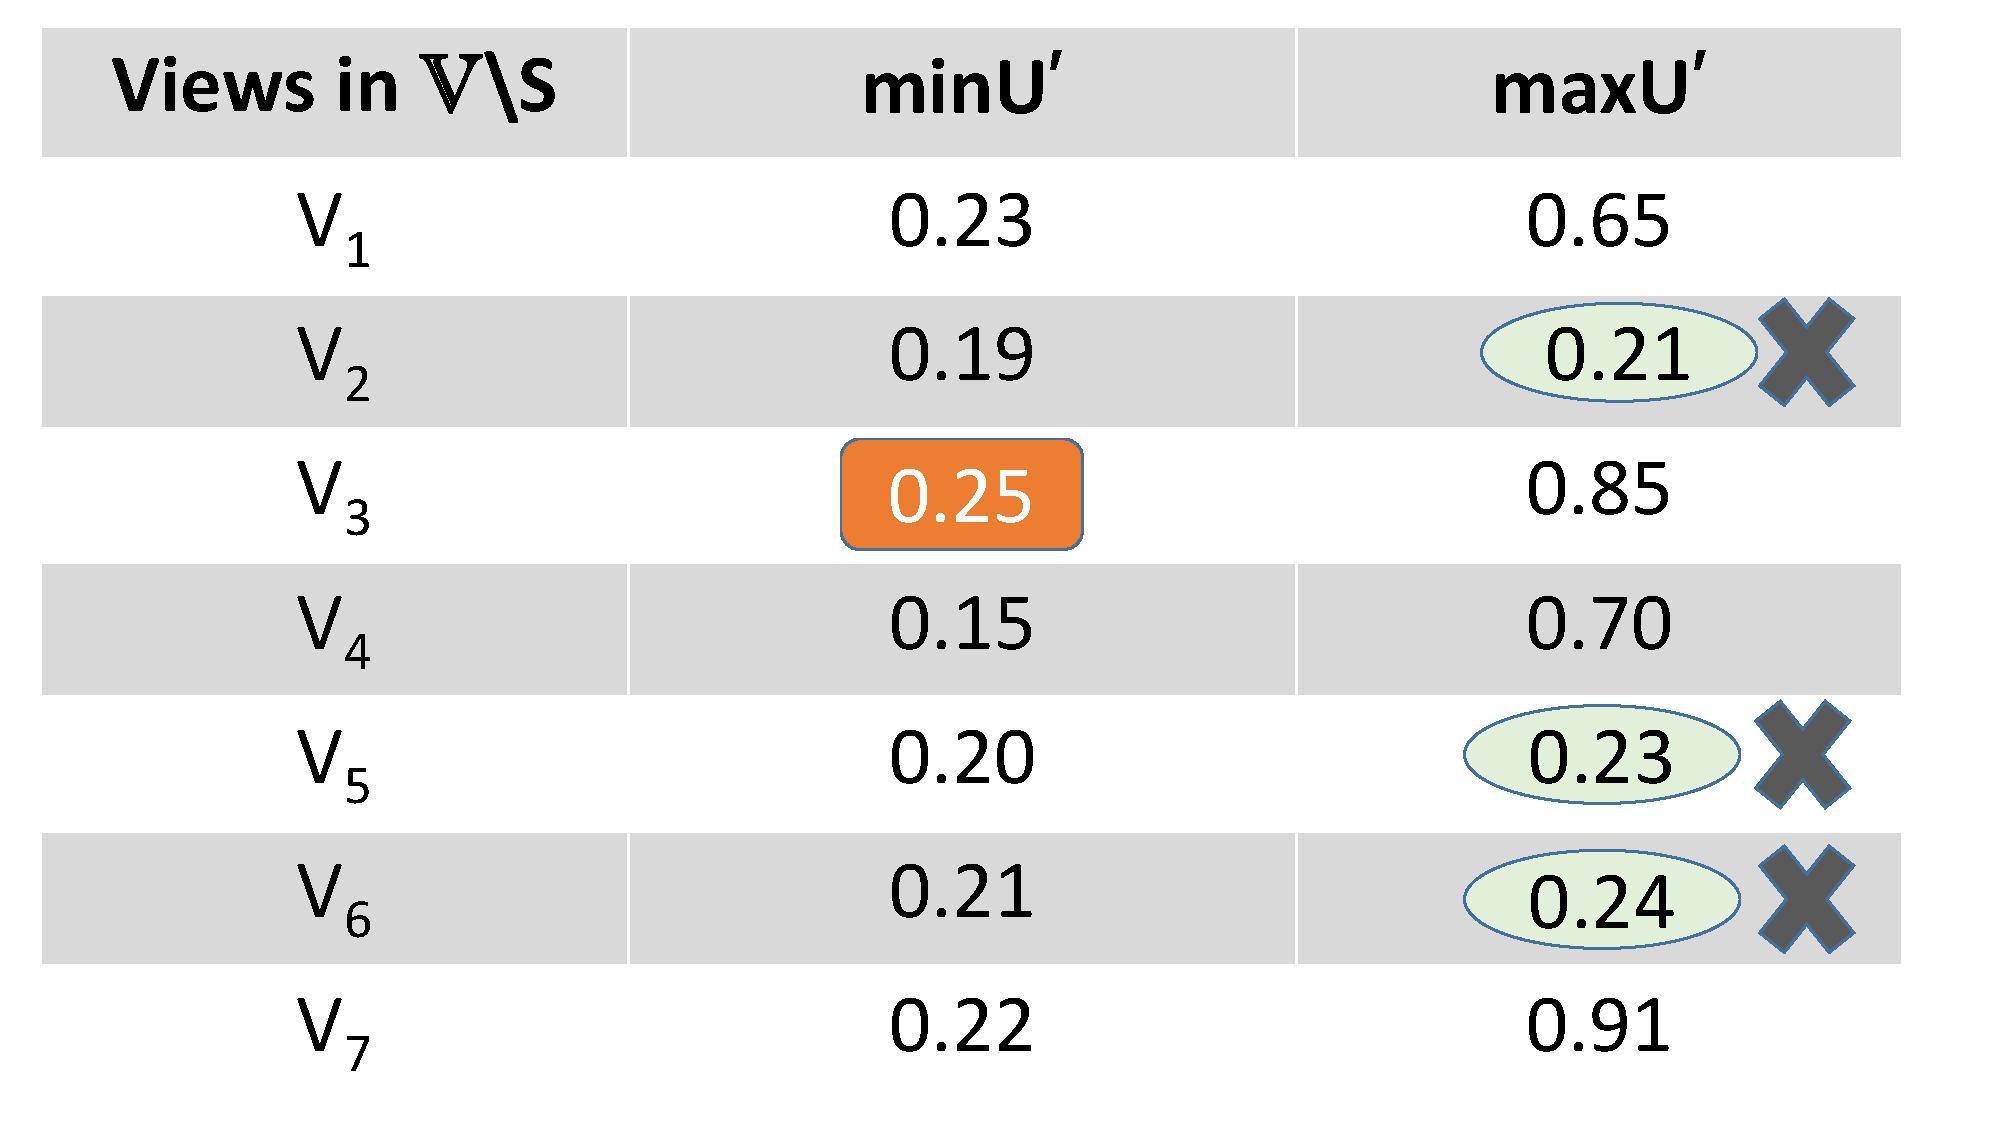
\includegraphics[width=3in]{figures/results/Max-Min}
%	\caption{Max-Min Pruning: All views which has $ maxU' $ less than the maximum of $ minU' $ will be pruned}
%	\label{fig:Max-Min}
%\end{figure}

Particularly, max-min utilizes the maximum and minimum bound on the importance score $I(V_i)$. 
%
%\mas{discuss bound}\note{you mean why the upper bound is $\sqrt{2}$}
Clearly, the minimum utility score is $I_0 = 0$, whereas the maximum utility value $I_u$ a view can score is computed as $I_u = \sqrt{2}$ (Sec. ~\ref{subsec:problem_definition}). 
%
Using those bounds, in each iteration the maximum $maxU(V_i)$ and minimum utility $minU(V_i)$ score for each view $V_i \in X$ is calculated as:
\[
 	maxU\left(V_i\right)= \left(1-\lambda\right) \times I_u\left(V_i\right) + \lambda \times setDist\left(V_i, S\right) 
\]
%\bigskip
\[	
minU\left(V_i\right)= \left(1-\lambda\right) \times I_0\left(V_i\right) + \lambda \times setDist\left(V_i, S\right) 
\]
Accordingly, the maximum value of $minU$ is recorded. 
%
Then, if $maxU$ of any candidate view is less than the maximum of $ minU$, then that view is pruned. 
%
%
%\mas{example is too simple - i think should be deleted} \note{both figure and text should be deleted or just text?}
%Figure \ref{fig:Max-Min} shows one simple iteration in which, the maximum value of $minU$ is $0.25$. 
%%
%Hence, all the views with $maxU$ value less than $0.25$ are pruned without executing their corresponding queries.
%%
%Once the actual importance score is calculated for the remaining views, then the view with highest utility score is selected and added to $S$.



\eat{ %hak version
The Max-Min pruning technique utilizes the maximum and minimum bound on the importance score. The maximum utility value $I_u$ a view can score is computed as $I_u = \sqrt{2}$,  and the minimum utility score is $I_0 = 0$. Using those bounds, in each iteration maximum and minimum utility score is calculated for each view in X as :
}

\eat{%hak version
\[
 	maxU'\left(V_i\right)= \left(1-\lambda\right).I_u\left(V_i\right) + \lambda.setDist\left(V_i, S\right) 
\]
%\bigskip
\[	
minU'\left(V_i\right)= \left(1-\lambda\right).I_0\left(V_i\right) + \lambda.setDist\left(V_i, S\right) 
\]

The maximum value of the $minU$ is recorded. If $maxU'$ of any candidate view is less than the maximum of $ minU'$, then that view is pruned. As shown in Figure \ref{fig:Max-Min}, the maximum value of $minU'$ is $0.25$. Hence, all the views with $maxU'$ value less than $0.25$ are pruned and view queries are generated only for the remaining views. Once the actual importance score is calculated for the remaining queries, the DiVE-Greedy algorithm selects the view with highest utility score to be added in S. Thus, the set of views computed by DiVE-Greedy using pruning is same as the one calculated without pruning.
}

\setlength{\textfloatsep}{0pt}% Remove \textfloatsep
\begin{algorithm}[t]
	\SetAlgoLined
	\KwIn{Set of views V and result set size k }
	\KwOut{Result set $ S \geq V $, |S| = k}  
	$S \leftarrow $ Result set of only importance or only diversity\;
	$X \leftarrow  \left[V \backslash S\right]$\;
	$F_{current} \leftarrow 0 $\;
	$  improve \leftarrow  True $\;
	\While{improve = True}{
		%		\If{Pruning = True}{
		%			$ enablePruning $\;
		%		}
		\For{$i$ in set $X$}{
			$ S' \leftarrow S $\;
			\For{$j$ in set $S$}{
				\If{ $ F\left(S'\right) < F\left(S \backslash S[j] \cup X[i]\right) $}{
					$ S'  \leftarrow S \backslash j \cup X[i] $  \;
				}
			}
			\If{ $ F\left(S'\right) > F\left(S\right) $}{
				$ S  \leftarrow S'$
			}
		}
		\eIf{ $ F\left(S\right) > F_{current} $}{
			$ F_{current}   \leftarrow F\left(S\right) $\;
			$  improve \leftarrow  True $\;
		}{
		$  improve \leftarrow  False $\;
	}
}
return S
\caption{\textit{DiVE} Swap}\label{DiVE-Swap}
\end{algorithm}


%
%This leads to two extreme baseline solutions, one based only on the importance score of the views which is called \textbf{\textit{"Linear-Importance"} } and second based on only diversity score of the views which is called \textbf{\textit{"Greedy-Diversity"}}. 
%
%Instead of uses one of those two extrem, \textit{DiVE} scheme employed hybrid function for evaluating top-k views which captures both the importance as well as diversity. Moreover, DiVE also equipped with pruning scheme which can prune a large number of queries without reducing the quality of the result. Our proposed DiVE scheme described below. 


%In order to capture both importance and diversity in the recommended top-k views, \textit{DiVE} employs a greedy construction algorithm to iteratively select views that maximize the hybrid objective function $F\left(S\right)$ as presented in equation 3, and it is called as \textbf{\textit{DiVE-Greedy}} scheme. 
%
%The details of the \textit{DiVE-Greedy} scheme are given in Algorithm \ref{DiVE-Greedy}. 
%%
%The key ingredient of any Greedy algorithm for solving an optimization problem is the objective function itself that needs to be maximized. In particular, \textit{DiVE-Greedy} initializes the set S with two most distant views. The distance between all the views is calculated using the distance function as given in equation 2. 
%%
%In each iteration, a new candidate view is selected from remaining views X and added to S. 
%
%Thus, \textit{DiVE-Greedy} assigns a utility score to each candidate view which is based on the hybrid objective function $F\left(S\right)$ as defined in equation \ref{objectif_function}. 
%
%The utility score of each candidate view $V_i$ in X is computed as: 
%
%\begin{equation}
%U\left(V_i\right)= \left(1-\lambda\right).I\left(V_i\right) + \lambda.setDist\left(V_i, S\right)
%\label{utility_each_candidate}
%\end{equation}
%
%Where $ setDist\left(V_i, S\right) = \dfrac{1}{|S|} \sum_{\underset{V_j \in S}{j=1}}^{|S|} D\left(V_i, V_j\right) $
%\newline
%
%Thus, the view with highest utility score in each iteration is selected and added to S.
%
%%\textit{DiVE-Greedy scheme costs.} There are four types of costs that required to run \textit{DiVE} scheme, as follows:
%%
%%\begin{itemize}
%%	\item Query cost $C_Q$: Cost that needed for the query execution, the cost of $C_Q$ depends on the query itself and the number of rows (tuples) of the dataset. This cost depends on CPU and I/O cost but it dominated by I/O costs. 
%%	\item Deviation/importance cost $ C_I $: The deviation computation cost is relatively cheap due to this cost only compute the probability distribution of each view and calculate the distance between two probability distribution of views (target view and reference view). The deviation equation can be seen in equation 1. This cost only from CPU costs.
%%	\item Diversity cost $C_D$: Cost which required not only the computation of dissimilarity between two context views but also for whole diversity computation. This cost also only from CPU costs. $C_D$ depends on the number of views and the diversity algorithm that used, e.g. Greedy construction is cheaper than Swap, the cheapest is Random Algorithm. 
%%	\item Visualization cost $C_V$: Cost which needed for plotting visualization and it only depends on CPU cost. 
%%\end{itemize}


%
%The costs of Greedy Construction algorithm has two components which are the query execution cost $C_Q$ that computing the importance score of view and the diversity cost $C_D$ that computing set distance of each view from the views already in S. The complexity of query execution cost is $ O$($n$) as the content of each view is generated only once. Meanwhile, the diversity cost $C_D$ is $ O$($kn$) where k is the size of subset of views S and $ n $ is the number of all possible views.
%
%Traditional diversification method applied approach such "process-first-diversity-next" which leads to generating all possible views and computing the importance score in advance, then the diversity is executed next. Although, greedy algorithm is very ent, however, as the number of attributes $\mathbb{A}$, measures $\mathbb{M}$ and aggregate functions $\mathbb{F}$ increase, the number of views that need to be generated grows exponentially. Hence, without a good strategy, \textit{DiVE-Greedy} suffers from the high costs of query execution. 
%
%Therefore, to overcome this issue, \textit{DiVE-Greedy} employs static pruning strategy as elaborated next. 

% ============================================== %
% PROPOSED METHODS %
% ============================================== %


\subsection{The DiVE-Swap Scheme}
\label{subsec:dive-swap}

Naturally, our DiVE-Greedy scheme described above will achieve a high pruning power for high values of $\lambda$ (i.e., diversity is assigned a high weight).
%
However, that pruning power diminishes for low values of $\lambda$ (i.e., importance is assigned a high weight).
%
That discrepancy in performance happens because of two reasons: 
%
(1) the constructive and iterative nature of the greedy algorithm, and (2) utilizing the upper bound on importance $I_u$ when computing $maxU(V_i)$. 
%
To explain those reasons, recall that the amount of pruning is shaped by the maximum value of $minU(V_i)$.
%
Now, consider an extreme case, in which $\lambda = 0.0$. 
%
In that case, all values of $minU(V_i)$ will also be equal to zero, and no pruning will take place. 
%
Similarly, for low values of $\lambda > 0$, the maximum value of $minU(V_i)$ will still be low, leading to limited pruning. 
%
That pruning is further reduced when combined with a high value of $I_u$ as it leads to all views acquiring high $maxU(V_i)$ and cannot be pruned.  
%
To address those limitations, we propose an adaptive scheme for setting $I_u$ in Sec.~\ref{subsec:adaptive-pruning}, and  orthogonally introduce our {\em Swap}-based DiVE scheme next.

\eat{
Since Greedy is constructive type algorithm, it contructs the set S by adding a new candidate view, there is no guarantee that the new view selected in each iteration is the best view for the objective function $F(S)$. It is because the view which has the highest utility score not necessary be the best one that improve the objective function $F(S)$ (e.g: local optimum). To overcome that issue, we proposed other schemes which based on swap technique.
}

The DiVE-Greedy algorithm presented in the previous section is of the constructive type. 
%
That is, it starts with an empty set of views and incrementally constructs it by adding one view at a time. 
%
To the contrary, our DiVE-Swap presented in this section falls under the {\em local search} type of algorithms. 
%
In general, a local search algorithm starts out with a complete initial solution and then attempts to find a better solution in the neighborhood of that initial one. 
%
Like constructive algorithms, local search algorithms are also widely used in solving optimization problems including diversification. 
%
For instance, the Swap local search method has been utilized to maximize diversity \cite{Drosou, Vieira2011}, and in this paper, we further expand it to our DiVE scheme. 

The basic idea underlying DiVE-Swap is to start with an initial set $S$ of size $k$ and then iteratively modify the set $S$ in order to improve the value of the objective function $F(S)$. 
%
One of the main design criteria in local search algorithms is the choice of the initial solution. 
%
In DiVE-Swap, we consider two natural variants: 1) {\em DiVE-iSwap}, and 2) {\em DiVE-dSwap}. 
%
In DiVE-iSwap, $S$ is initialized with the $k$ views that maximize importance and can be easily obtained using our baseline Linear-Importance (Sec. ~\ref{subsec:baseline}).
%
Alternatively, in DiVE-dSwap, $S$ is initialized with the $k$ views that maximize diversity using Greedy-Diversity (Sec.~\ref{subsec:baseline}).
%

Apart from the initialization approach, both variants work similarly. 
%
Particularly, in each iteration, each unselected view $X_i \in X$ is interchanged with all the selected views in $S_j \in S$ (Algorithm \ref{DiVE-Swap} line 9). 
%
That is, the overall hybrid objective is computed for $F(S \backslash S_j \cup X_i)$.  
%
Then the one interchange that leads to the highest new value for $F$ is applied and $S$ is updated accordingly (Algorithm \ref{DiVE-Swap} line 10). 
%
Such iterations are repeated until no more views can be swapped between $X$ and $S$, which is reached when no further improvement is achieved in the value of $F$.   

\eat{
Swap is local search type algorithm and it has been known and used to maximize diversity in the literature \cite{Drosou, Vieira2011}. This algorithm starts with a complete initial set $S$, and try to achieve better result by interchanging the remaining views in $X$ to the current set $S$. If a view in $X$ is able to improve objective function value $ F $($ S $), then this view can be joined to the current set and one view in the current set that has the lowest contribution to the $ F $($ S $) will be removed. The details of \textit{DiVE-Swap} algorithm can be seen in Algorithm \ref{DiVE-Swap}.

Due to Swap need a complete initial set, we proposed two types of Swaps which are: 1) \textbf{\textit{DiVE-iSwap} }, the underlying behind this sheme is, it has the initial set from the result of Linear-Importance which is importance score maximized.  2) \textbf{\textit{DiVE-dSwap}} which is quite similar to DiVE-iSwap, however, this scheme is initialized by results of Greedy-Diversity, which is diversity maximized. Those two swaps have different initial set and in each iteration, the candidate view is exchanged from $X$ to the current set $S$ till the $F(S)$ is maximized as given in Eq \ref{objectif_function}. 
}
% %explain why initialization by Importance and Initialization by Diversity

In comparison to DiVE-Greedy, DiVE-Swap incurs the same query processing cost $C_Q$. 
%
Furthermore, it incurs even higher $C_D$ cost for computing diversity, which can reach up to $ O\left(kn^2 \right) $. 
%
However, as described next, DiVE-Swap offers a valuable opportunity for maximizing the number of pruned views, and in turn reducing the query processing cost $C_Q$, which is the dominant factor in determining  efficiency.   

\eat{
\textbf{\textit{DiVE-Swap cost}}. The costs of Swap algorithm is also depend on the query execution time $C_Q$ of all possible views and the diversity computation $C_D$. The query cost $C_Q$ is executed only once but the cost is high due to it needs I/O cost. However, the complexity of diversity computation $C_D$ is $ O\left(k^2 \right) $ and the number of distance computation depends on the number of iterations of the swap and the number of views in $X$ which can be seen in Algorithm \ref{DiVE-Swap} line 5. In the worst case, swap algorithm can perform $ O\left(k^n \right) $ iterations. Without any pruning scheme, the cost of \textit{DiVE-iSwap} is same as \textit{ DiVE-dSwap} due to those both schemes are using same technique only different in the initial set. 
}


\subsection{Optimized DiVE-dSwap}
\label{subsec:dive-dswap}

%% role of initialization
While both DiVE-iSwap and DiVE-dSwap described above incur the same cost, they offer substantially different performance when combined with pruning techniques. 
%
Particularly, consider DiVE-iSwap, which is initialized with the $k$ views that maximize importance. 
%
To select those views, all possible views have to be generated first, which in turn requires processing all their corresponding queries. 
%
Hence, DiVE-iSwap simply eliminates all opportunities for pruning as all views are executed in the initialization phase. 
%
To the contrary, DiVE-dSwap is initialized with the $k$ views that maximize diversity.
%
To select that initial set, no query execution is needed and the processing is limited to computing the context-based deviation distances, which is significantly low compared to query processing. 
%
Hence, DiVE-dSwap allows integrating effective pruning techniques, as described next. 

%% how it leads to pruning 
Recall that under DiVE-dSwap, in each iteration a view $X_i \in X$ is selected to replace a view $S_j \in S$. 
%
The criterion for that selected view is to improve $F\left(S\right)$. 
%
That is, $F(S \backslash S_j \cup X_i) >  F(S)$. 
%
Hence, the task is to find that {\em top-1} pair of views $<X_i, S_j>$ that provide the maximum improvement in $F\left(S\right)$ once interchanged. 
%
Without pruning, that requires iterating through $S$ and $X$ simultaneously and computing $F$ for each pair, which requires processing and generating each view in $X$. 
%
To avoid such expensive processing and enable pruning, the following steps are taken. 
%

A list $L$ is created for all possible swap pairs $<X_i, S_j>$, where $L$ is sorted based on the diversity achieved if the swap is to be made. 
%
%
Notice that up to this point the only processing needed is to compute diversity without any query execution to evaluate the importance of any $X_i$. 
%
%
Given that setting, the task is clearly similar to top-k query processing, for which numerous optimization techniques are proposed (e.g., \cite{Fagin:2003:CTK:644108.644113, Ilyas:2008:STK:1391729.1391730}).
%
Particularly, to find the {\em top-1} view, each view $X_i$ is initially assigned an importance equal to the upper bound $I_u$. 
%
In turn, the upper bound of $F\left(S\right)$ achieved by $X_i$ is computed as: $maxF(S \backslash S_j \cup X_i)$, which is based on the actual diversity achieved by the swap, and the upper bound on importance.
%
As such, $maxF(S \backslash S_j \cup X_i)$ is compared against $F(S)$, leading to one of the following two cases:
%
If $maxF(S \backslash S_j \cup X_i)$ > $F(S)$, then the swap $<X_i, S_j>$ can ``potentially'' improve $F\left(S\right)$. 
%
Hence, at that stage the view $X_i$ needs to be generated in order to evaluate its actual importance $I(X_i)$. 
%
Otherwise, the pair $<X_i, S_j>$ is pruned if: $maxF(S \backslash S_j \cup X_i) < F(S)$.

Simply put, if the upper bound  $maxF$ achieved by that swap is still less than the current $F(S)$, then the actual $F(S \backslash S_j \cup X_i)$ is guaranteed to be less than $F(S)$ and the pair $<X_i, S_j>$ can be safely ignored. 
%
More importantly, since the $L$ is sorted by diversity, then the next views are also guaranteed to provide no improvement and that iteration of DiVE-dSwap reaches {\em early termination}.  
%
Hence, for all the remaining views no query processing is needed, which significantly reduces the overall cost. 

\noindent{\bf DiVE-dSwap vs. DiVE-Greedy:} At this point, it is especially important to examine and contrast the pruning power achieved by each of DiVE-Greedy and DiVE-dSwap. 
%
For DiVE-Greedy, recall that pruning is attained for those views where: $maxU(V_i) < maxminU$. 
%
However, since DiVE-Greedy is a constructive algorithm, the set $S$ is incrementally constructed iteration by iteration until $|S|=k$. 
%
Hence, in the first iterations $S$ has a very small number of selected views with a minimum of $|S|=2$. 
%
Naturally, when $S$ is a small set, then most of the remaining unselected views in $X$ are expected to exhibit high diversity, since the majority of them will be very dissimilar from the small set of views in $S$.
%
Accordingly, for most of the views in $X$, the value $maxU(V_i)$ will be relatively high, due to achieving high score on diversity. 
%
Hence, most views will fail to satisfy the pruning condition and are consequently executed incurring high query processing cost. 

To the contrary, DiVE-dSwap is initiated with a set $S$ of $k$ diverse views. 
%
Hence, it will initially have a reasonably high $F(S)$. 
%
Moreover, many views in $X$ will be ``close'' to some view in $S$. 
% 
Hence, the swaps that involve those views will score low on diversity, and in turn low $maxF$.
%
Since pruning happens when $maxF(S \backslash S_j \cup X_i) < F(S)$, the combination of those two factors above (i.e., high $F$ and low $maxF$) allows for many views satisfying the pruning condition, which improves the pruning power of DiVE-dSwap. 
%
That pruning power can be further improved by relaxing the assumption about maximum importance $I_u$, as described next.



%% how pruning is done

%% contrast to greedy
\eat{
In terms of pruning, two our proposed Swap are quite different. \textit{DiVE-iSwap} utilize the results of Linear-Importance as the initial set. Hence, this algorithm cannot escape from executing all queries due to Linear-Importance needs to execute all possible views to get the results. However, the second proposed swap algorithm, \textit{ DiVE-dSwap} is initialized by the result of Greedy-Diversity. This algorithm does not execute any query to generate the results. Therefore, we can employ pruning technique in \textit{ DiVE-dSwap} by leveraging the properties of importance and diversity.

While in \textit{DiVE-Greedy-Static}, the maximum and minimum bound of importance score are utilized, in this scheme, only maximum bound $I_u$ is used. This \textit{ DiVE-dSwap-Static} also leverage both the importance and diversity score of a candidate view to decide whether a view query should be executed or not. The details \textit{ DiVE-dSwap-Static} technique explained as follows:

\begin{itemize}
	\item Since the initial set of \textit{ DiVE-dSwap} is the result of Greedy-Diversity, all query views in the initial set need to be executed in order to get the objective function $F(S)$ of the current set $S$. The $F(S)$ of current set will be compared to the new $F(S)$ after exchanging a view as shown in Algorithm \ref{DiVE-Swap} line 9.
	\item In order to confirm that exchanging process starts from the candidate view that has highest score of diversity, all views in $X$ is sorted based on $ setDist\left(V_i, S\right)  $ before start exchanging view from $ X $ to the current set $S$. This is called as \textit{"top-1"} technique. 
	\item To start exchanging view, the importance score must be known by executing the query of the candidate view. Instead of executing query view, the maximum bound of importance score is used to compute the utility score of each view as in \textit{DiVE-Greedy-Static} technique. Hence, the result is not the actual utility score but $ maxU' $, which defined as: $ 	maxU'\left(V_i\right)= \left(1-\lambda\right) \times I_u\left(V_i\right) + \lambda \times setDist\left(V_i, S\right) $.
	\item The exchanging process is started by comparing $F(S)$ of the current set to $F(S)$ of new set as given in Algorithm \ref{DiVE-Swap} lines 9 - 10. The $F(S)$ of new set is computed by Eq \ref{objectif_function} while $ maxU' $ is used as the utility score of candidate view from $ X $.
	\item If using importance score $I_u$ candidate views in $X$ cannot improve the objective function $F(S)$ to the current set $S$, those views will be pruned. 
\end{itemize}

This technique is valid due to if the maximum score of importance $I_u$ is used and that view cannot improve $F(S)$ of the current set, then there is no reason to execute the view query to get the importance score $I$ ($I \leq I_u$) . 

%This pruning scheme is called \textbf{\textit{DiVE-dSwap-Static}}.

All proposed pruning techniques including \textit{DiVE-Greedy-Static} and \textit{DiVE-dSwap-Static} are using static value $I_u$ as the bound. However, the pruning performance cannot be optimal while the value of $I_u$ is far away from the actual maximum of importance score in database. To overcome this issue, we proposed adaptive pruning scheme as described in the next section. 
}
% Compare with Greedy in terms of pruning performance%

%\subsection{Adaptive Pruning Scheme}
%%Premble
%
%Two pruning techniques \textit{DiVE-Greedy-Static} and \textit{DiVE-dSwap-Static} have been presented. Those two static pruning techniques utilized maximum bound $I_u$ to determine whether the query view need to be executed or not. Only view that can improve the $F(S)$ of the current set while using $I_u$ will be executed otherwise those are pruned. However, one drawback using static bound $I_u$ in pruning technique is that if the bound is far away from the maximum score of importance score in the dataset, the pruning cannot work optimal. To overcome this issue, instead of using static bound $I_u$, we proposed adaptive pruning scheme that automatically adapts the bound to the real maximum importance score in the dataset. 
%
%The adaptive pruning technique is utilizing the maximum bound $I_u$ as in static pruning as a first initial bound, however, this bound is changed to the real value of maximum importance score after some query views are executed. The problem occurs when the executed views have a small importance score and it is far below from the most views in the dataset. Thus, it brings the pruning out of control because while the bound is very low and there are many views in dataset have higher importance score compared to the bound, it may result wrong prune. Hence, DiVE needs the strategy to ensure that the bound score is close as possible to the maximum importance score in the dataset while it is changed. One of the approach that can be used is by selecting sample views to be executed then get the maximum importance score of the view from those sample. This brings us to the question of how many samples are needed in order to hit a view that has a maximum score from the dataset.
%
%There are several literatures have been mentioned related to the confidence interval and the number of samples in the normal distribution [cite]. However, the importance score of candidate views in $X$ is not in normal distribution. The highest importance score is the upper bound of maximum importance $I_u$ whereas the lowest is 0, and it is long tail distribution. Hence, we adopt the sampling method from this [cite] as our data is not in normal distribution, it is called as prediction interval ($ PI $) which is similar to a confidence interval in normal distribution. The relation between $ PI $ and the number of samples defined as in equation \ref{prediction-interval}.
%
%\begin{equation}
%	PI= \dfrac{\left(N-1\right) }{\left(N + 1\right)}, where\, N = Number\, of\, samples
%	\label{prediction-interval}
%\end{equation}
%
%In general, analyst may use $ PI $ start from 80 to 99. While $ PI $ = 80\% states that there are 9 sample views need to be executed, 85 \%, 90\%, 95\%, 97\%, and 99\% means 12, 20, 40, 60, and 200 samples need to be executed respectively. 
%
%\textit{Adaptive pruning flows}. We employ adaptive pruning technique to both schemes, \textit{DiVE-Greedy} and \textit{DiVE-dSwap}. In case of Greedy technique, the upper bound $I_u$ is used at the first time, thus the value $I_u$ is changed to maximum importance score from the samples of views which are executed. In order to change the bound value, the number of samples that need to be executed depends on the $ PI $ value which defined by the analyst. Futhermore, the bound is changed while in the next view execution that there is a view which has importance score higher than the used current bound.
%
%For adaptive pruning technique in \textit{DiVE-dSwap}, the details is described as follows:
%
%\begin{itemize}
%	\item Firstly, as in \textit{ DiVE-dSwap-Static} that all query view in the initial set are executed in order to get the objective function $F(S)$ of the current set $S$ and all candidate views in $X$ is sorted based on $ setDist\left(V_i, S\right)  $.
%	\item $ maxU' $ of each view is computed by utilizing the maximum bound of importance score $I_u$, where $ maxU'\left(V_i\right)= \left(1-\lambda\right) \times I_u\left(V_i\right) + \lambda \times setDist\left(V_i, S\right) $. 
%	\item All views in $X$ is exchanged to the current set one by one and a view that can improve $F(S)$ will be executed in order to get the actual value of importance. 
%	\item The bound is changed while the number of views which are executed reaches the number of sample based on the PI which determined by analyst. For instance, analyst may use PI = 97\%, hence, bound is changed while the sum of number of candidate views and th number of views in the initial set equal to 60 views. While it reaches to 60 views, the bound is replaced by the maximum importance score of executed views.  
%	\item If in the next query view execution, there is a view which has higher importance score than the bound. Thus, the bound is changed to that score. 
%\end{itemize}
%
%%To check the performance of our proposed pruning techniques
%
%In this work, adaptive pruning in Greedy is called \textit{DiVE-Greedy-Adaptive} wheras in Swap is called \textit{DiVE-dSwap-Adaptive}.

%
%
%$maxU'$ of each candidate view is computed first using $current bound$ before executing the query, view which cannot make an improvement to the S while using $current bound$ will never be executed and it will be pruned
%  
%In order to get better performance of pruning scheme, instead of using static $max_I = \sqrt{2} $, we proposed Adaptive Pruning scheme, that can adapt the value of $max_I$ to the real values in the dataset. In order to estimate the $max_I$ which can close to the real value in the dataset, we use sampling method. 


%For instance, in the \textit{DiVE-dSwap-Adaptive-Pruning}, $max_I$ is initialized by $ \sqrt{2} $. If the view by using $max_I$ can improve the objective function value in the current set $S$, the real Importance score of this view will be computed which is by executing the query of its view. For instance, after executing its query, the real Importance value is 0.25, by using $ \alpha= 0.8 $, the $ EWMA_t  $ will be $ (0.8 *0.25) + ((1- 0.4)*\sqrt{2}) = 0.48 $, and the current $max_I$ will be set to 0.48, and it will be updated continuously. This EWMA method able to set the value of $max_I$ as close as the real values in the dataset, it should make pruning scheme works better. 

% % Pruning Pseudocode

%\begin{algorithm}
%	%	\SetAlgoLined
%	%	\KwIn{Set of views V and result set $S$ize k }
%	%	\KwOut{Result set $ S \geq V $, |S| = k}  
%	%	$S \leftarrow $ Result set of only importance or only diversity\;
%	%	$X \leftarrow  \left[V \backslash S\right]$\;
%	%	$F_{current} \leftarrow 0 $\;
%	%	$  improve \leftarrow  True $\;
%	$ max_b  \leftarrow\sqrt{2} $\;
%	%$ X' \leftarrow [] $\;
%	\For{$i$ in set $X$}{
%		\For{$j$ in set $S$}{
%			$ d  \leftarrow setDist\left(X[i],S \backslash S[j]\right) $\;
%			$ 	newX \leftarrow [S[j], X[i], d]$\;
%			$ 	X'.append(newX)$\;
%		}
%	}
%	$ 	X' \leftarrow sorted\_by\_d(X') $\;
%	$ S' \leftarrow S $\;
%	\eIf{ $ max_b == \sqrt{2} $}{
%		\For{$i$ in set $X'$}{
%			
%			\If{ $ F\left(S'\right) < F\left(S \backslash X'[i][0] \cup X'[i][1], max_b\right) $}{
%				$ 	X''.append(X'[i][1])$\;
%			}
%		}
%		
%		$n \leftarrow pi - len(S)$\;
%		$samples \leftarrow X''[0\colon n]$\;
%		$maxI\_S \leftarrow get\_maxI(S)$\;
%		$maxI\_samples \leftarrow get\_maxI(samples)$\;
%		
%		\If{ $ maxI\_S > maxI $}{
%			$ maxI \leftarrow maxI\_S$
%		}
%		\If{ $ maxI\_samples> maxI $}{
%			$ maxI \leftarrow maxI\_samples$
%		}
%		$max\_b \leftarrow maxI$	
%		
%		\For{$i$ in set $X''$}{
%			\For{$j$ in set $S$}{
%				\If{ $ F\left(S'\right) < F\left(S \backslash S[j] \cup X''[i], max_b\right)  $}{
%					$ 	X'''.append(X''[i])$\;
%					$ I \leftarrow get\_I\_score(X''[i]) $\;
%					\If{ $ F\left(S'\right) < F\left(S \backslash S[j] \cup X''[i], I\right) $}{
%						$ S'  \leftarrow S \backslash j \cup X''[i] $  \;
%					}
%					\If{ $ I > max_b $}{
%						$ max_b \leftarrow I $
%					}
%				}
%			}
%		}
%		
%	}{ 
%	\For{$i$ in set $X'$}{$ .... $
%		%			\If{ $ F\left(S'\right) < F\left(S \backslash X'[i][0] \cup X'[i][1]\right) $}{
%		%				$ 	X''.append(X'[i][1])$\;
%		%			}
%		%			$ I \leftarrow get\_I\_(X''[i]) $\;
%		%			\If{ $ F\left(S'\right) < F\left(S \backslash S[j] \cup X''[i], max\_bound\right) $}{
%		%				$ S'  \leftarrow S \backslash j \cup X''[i] $  \;
%		%			}
%		%			\If{ $ I > max\_bound $}{
%		%				$ max\_bound \leftarrow I $
%		%			}
%		
%	}
%	
%}
%
%\If{ $ F\left(S'\right) > F\left(S\right) $}{
%	$ S  \leftarrow S'$
%}
%return S
%\caption{\textit{DiVE} SwapD Pruning}\label{DiVE-dSwap-Pruning}
%\end{algorithm}

%In order to apply pruning in \textit{DiVE-dSwap}, as in the Greedy technique, we utilize the maximum bound of importance score $I_u$ to compute $ maxU' $ of each candidate views in $X$ which defined as:
%In each iteration, instead of computing a complete utility score for each view, only partial utility score is computed, as in equation \ref{partial_utility}. The partial utility score using actual value of diversity score and estimated value of importance score $max_I$ which is equal to $\sqrt{2}$.

%\begin{figure}
%	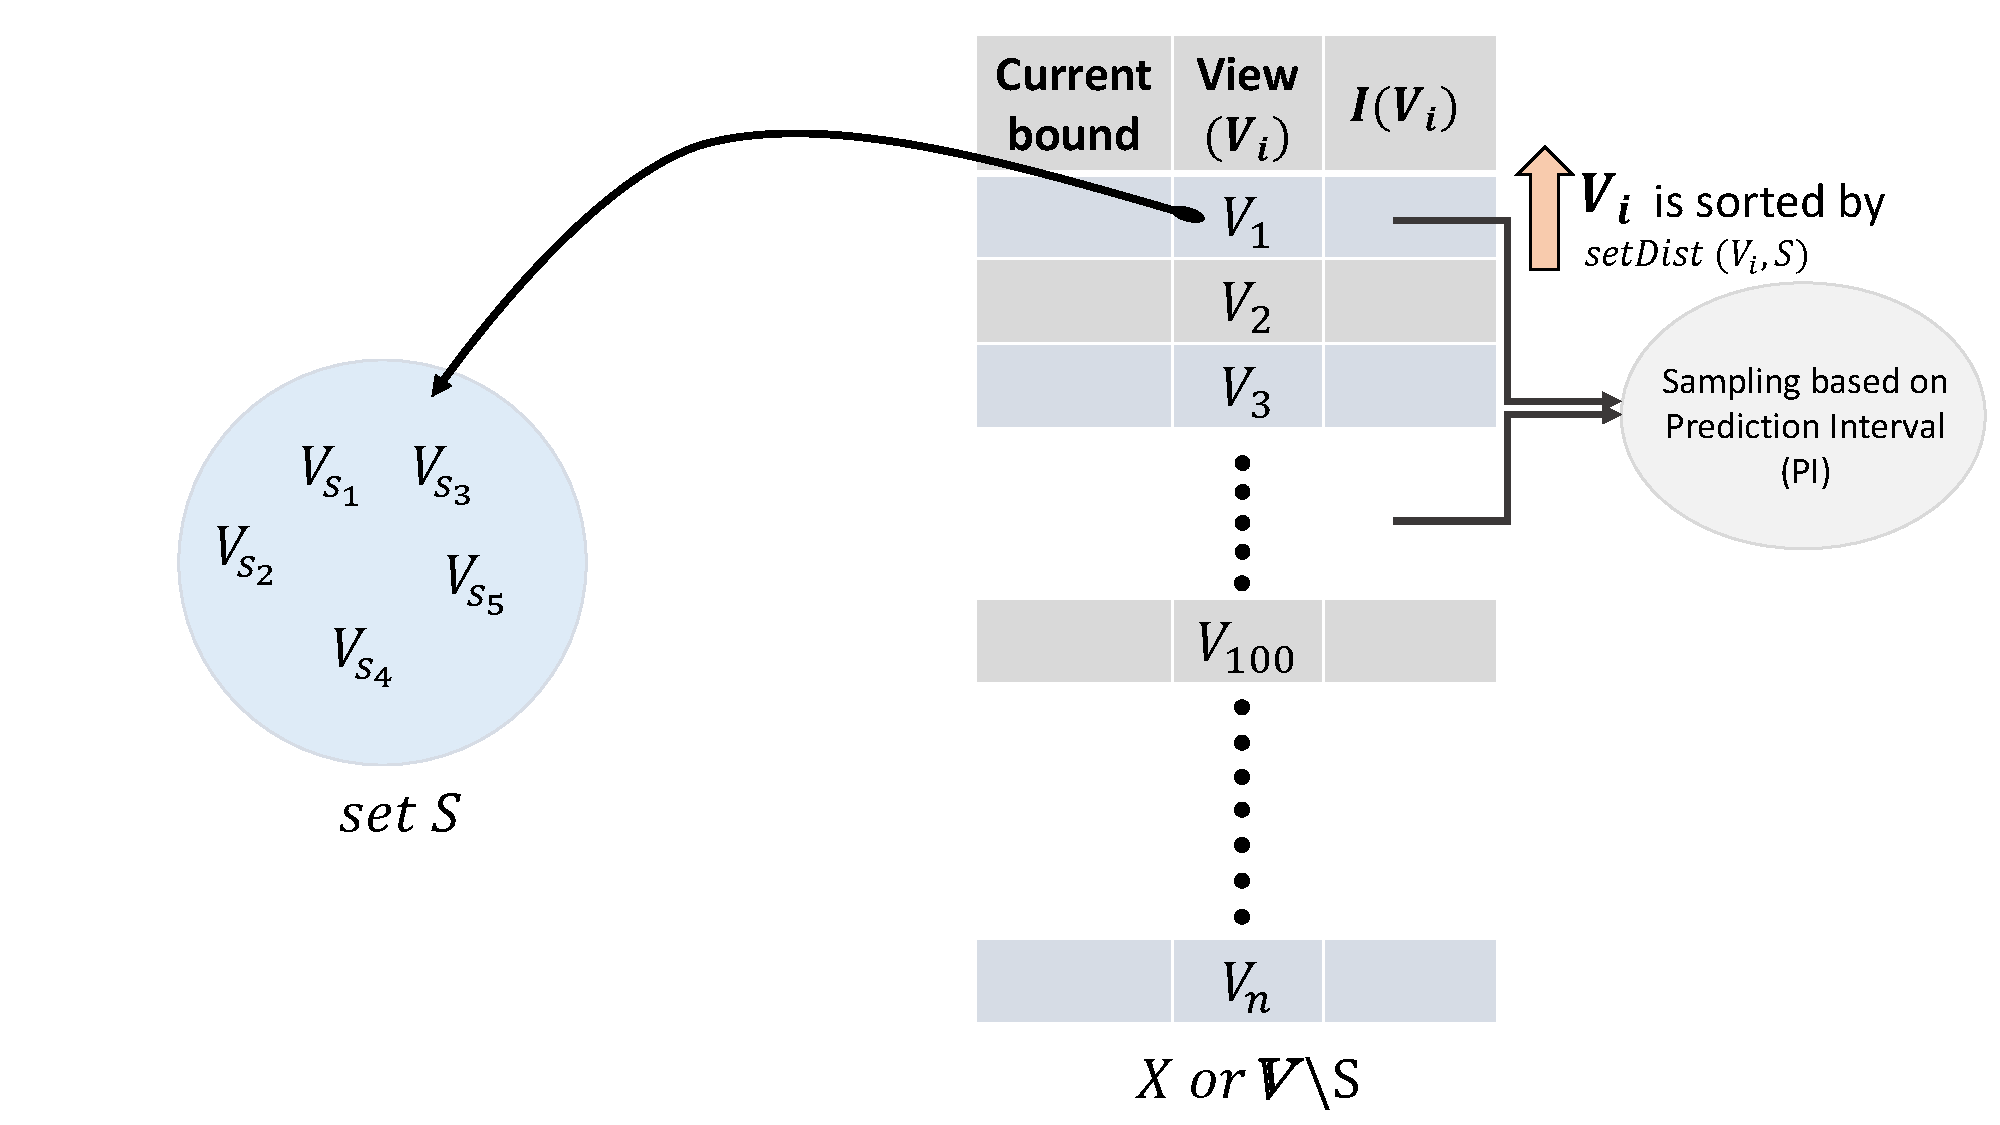
\includegraphics[width=3in]{figures/results/dSwap-Pruning}
%	\caption{dSwap-Pruning: Each candidate view has importance score and $ current bound $. The importance score of view will be generated only for view which its utility score is able to improve set $S$ while using $currentbound$ }
%	\label{fig:dSwap-Pruning}
%\end{figure}

%The idea behind pruning scheme is to minimize the query execution, which is by early prune low quality views. There are two main parameters in pruning scheme: 1) weight of $\lambda$ and 2) the max bound value $I_u$. 

%The weight of $\lambda$ is important due to it determines the contribution of importance score and diversity score. For instance, assume that an analyst wants to get set of views from view recommendation and she uses $\lambda$ = 0.7. The $\lambda$ value equal to 0.7 means that the diversity contribution to the utility score is 70\% and the contribution of importance score will be 30 \%, as it can be seen in equation \ref{objectif_function}. Thus, by setting the $\lambda$ to higher value, the contribution of importance score will be lower and more queries are pruned. This $\lambda$ value is determined by analyst, however, in this experiement 0.5 is used as the default. 
% ============================================== %
% PROPOSED METHODS %
% ============================================== %

\vspace{-7pt}
\subsection{Predictive Interval for Adaptive Bounds}
\label{subsec:adaptive-pruning}
%Premble


%% I_u and its drawbacks
In general, both the pruning schemes provided by DiVE-Greedy and DiVE-dSwap rely on the fundamental idea of evaluating the upper bound of the benefit provided by a view $V_i$ towards the objective $F$. 
%
If that maximum benefit is still not enough to consider $V_i$ to join $S$, then $V_i$ is pruned and its query processing cost is saved. 
%
Moreover, to evaluate that upper bound, both schemes compute the actual diversity offered by $V_i$ and instead of computing its actual importance, it is substituted with the maximum attainable importance score $I_u$. 
%
Naturally, overestimating  $I(V_i)$ leads to overestimating its benefit and consequently limited pruning power is achieved. 
%
Meanwhile, for most datasets, $I_u$ is in fact an overestimation of $I(V_i)$. 
%
Hence, our goal in this section to provide a tighter bound on $I(V_i)$, which allows for maximum pruning while maintaining the quality of the solution. 
 

Recall that $I_u$ is achieved when for each group $a_i$, the corresponding value $\frac{g_i}{G}$ in $P[V_{i}(D_R)]$ or $P[V_{i}(D_Q)]$ is zero. 
%
Hence, $I_u$ is a theoretical bound for the maximum importance achieved by any view in any dataset.
%
For most real datasets, however, that condition is rarely satisfied and the actual upper bound $I_{au}$ is typically much smaller than $I_u$. 
%
Meanwhile, a hypothetical pruning scheme that utilizes that actual upper bound $I_{au}$ is expected to deliver more pruning power than the schemes using the theoretical upper bound $I_u$, especially when $I_{au}  \ll I_u$.
%
In practice, however, that hypothetical scheme is not achievable since obtaining the value $I_{au}$ requires executing all the possible views, which is clearly in conflict with the goal of pruning.

Accordingly, rather than using overestimated $I_u$ or obtaining the actual $I_{au}$, our goal is to estimate $I_{au}$ with high accuracy and minimum number of query executions. 
%
In particular, given the set of possible views $\mathbb{V}$, the goal is to estimate the maximum importance $\bar{I}_{au}$ given by some view in $\mathbb{V}$. 
%
However, estimating the maximum value of a population is known to be a challenging problem, as opposed to estimating other statistics such as average or sum \cite{Hu:2009:EAT:1516360.1516487}.
%
That challenge is further emphasized when the values exhibited by the population are skewed and do not follow a typical normal distribution, which is typically the case for the importance value of views.
 %
 
Thus, instead of estimating $I_{au}$, we rely on {\em non-parametric predictive interval} models to determine its value with certain level of confidence without any assumption on the population \cite{Hu:2009:EAT:1516360.1516487}. 
%
To apply that model, some sample views are executed and the maximum importance observed in that sample is recorded as $\bar{I}_{au}$. 
%
To determine the number of samples, a {\em Predictive Interval (PI)} is to be defined, such that: 	
$PI= \dfrac{\left(m-1\right) }{\left(m + 1\right)}$, where $m$ is the number of samples. 
%

For instance, setting $m = 19$, results in PI = 90\%. 
%
That is, 90\% of the time, the importance value of an unseen view $V_i$ will be less than the maximum importance seen so far. 
%
Clearly, the higher the PI value, the higher the accuracy of $\bar{I}_{au}$, but also requires executing more views.  
%
In this work, we find that a value of $PI=97\%$ is able to strike a fine balance between minimizing the number of executed queries and maximizing the objective $F$, as shown next.


\eat{
Two pruning techniques \textit{DiVE-Greedy-Static} and \textit{DiVE-dSwap-Static} have been presented. Those two static pruning techniques utilized maximum bound $I_u$ to determine whether the query view need to be executed or not. Only view that can improve the $F(S)$ of the current set while using $I_u$ will be executed otherwise those are pruned. However, one drawback using static bound $I_u$ in pruning technique is that if the bound is far away from the maximum score of importance score in the dataset, the pruning cannot work optimal. To overcome this issue, instead of using static bound $I_u$, we proposed adaptive pruning scheme that automatically adapts the bound to the real maximum importance score in the dataset. 

The adaptive pruning technique is utilizing the maximum bound $I_u$ as in static pruning as a first initial bound, however, this bound is changed to the real value of maximum importance score after some query views are executed. The problem occurs when the executed views have a small importance score and it is far below from the most views in the dataset. Thus, it brings the pruning out of control because while the bound is very low and there are many views in dataset have higher importance score compared to the bound, it may result wrong prune. Hence, DiVE needs the strategy to ensure that the bound score is close as possible to the maximum importance score in the dataset while it is changed. One of the approach that can be used is by selecting sample views to be executed then get the maximum importance score of the view from those sample. This brings us to the question of how many samples are needed in order to hit a view that has a maximum score from the dataset.

There are several literatures have been mentioned related to the confidence interval and the number of samples in the normal distribution [cite]. However, the importance score of candidate views in $X$ is not in normal distribution. The highest importance score is the upper bound of maximum importance $I_u$ whereas the lowest is 0, and it is long tail distribution. Hence, we adopt the sampling method from this [cite] as our data is not in normal distribution, it is called as prediction interval ($ PI $) which is similar to a confidence interval in normal distribution. The relation between $ PI $ and the number of samples defined as in equation \ref{prediction-interval}.

\begin{equation}
	PI= \dfrac{\left(N-1\right) }{\left(N + 1\right)}, where\, N = Number\, of\, samples
	\label{prediction-interval}
\end{equation}

In general, analyst may use $ PI $ start from 80 to 99. While $ PI $ = 80\% states that there are 9 sample views need to be executed, 85 \%, 90\%, 95\%, 97\%, and 99\% means 12, 20, 40, 60, and 200 samples need to be executed respectively. 

\textit{Adaptive pruning flows}. We employ adaptive pruning technique to both schemes, \textit{DiVE-Greedy} and \textit{DiVE-dSwap}. In case of Greedy technique, the upper bound $I_u$ is used at the first time, thus the value $I_u$ is changed to maximum importance score from the samples of views which are executed. In order to change the bound value, the number of samples that need to be executed depends on the $ PI $ value which defined by the analyst. Futhermore, the bound is changed while in the next view execution that there is a view which has importance score higher than the used current bound.

For adaptive pruning technique in \textit{DiVE-dSwap}, the details is described as follows:

\begin{itemize}
	\item Firstly, as in \textit{ DiVE-dSwap-Static} that all query view in the initial set are executed in order to get the objective function $F(S)$ of the current set $S$ and all candidate views in $X$ is sorted based on $ setDist\left(V_i, S\right)  $.
	\item $ maxU' $ of each view is computed by utilizing the maximum bound of importance score $I_u$, where $ maxU'\left(V_i\right)= \left(1-\lambda\right) \times I_u\left(V_i\right) + \lambda \times setDist\left(V_i, S\right) $. 
	\item All views in $X$ is exchanged to the current set one by one and a view that can improve $F(S)$ will be executed in order to get the actual value of importance. 
	\item The bound is changed while the number of views which are executed reaches the number of sample based on the PI which determined by analyst. For instance, analyst may use PI = 97\%, hence, bound is changed while the sum of number of candidate views and th number of views in the initial set equal to 60 views. While it reaches to 60 views, the bound is replaced by the maximum importance score of executed views.  
	\item If in the next query view execution, there is a view which has higher importance score than the bound. Thus, the bound is changed to that score. 
\end{itemize}

%To check the performance of our proposed pruning techniques

In this work, adaptive pruning in Greedy is called \textit{DiVE-Greedy-Adaptive} wheras in Swap is called \textit{DiVE-dSwap-Adaptive}.
}
%
%
%$maxU'$ of each candidate view is computed first using $current bound$ before executing the query, view which cannot make an improvement to the S while using $current bound$ will never be executed and it will be pruned
%  
%In order to get better performance of pruning scheme, instead of using static $max_I = \sqrt{2} $, we proposed Adaptive Pruning scheme, that can adapt the value of $max_I$ to the real values in the dataset. In order to estimate the $max_I$ which can close to the real value in the dataset, we use sampling method. 


%For instance, in the \textit{DiVE-dSwap-Adaptive-Pruning}, $max_I$ is initialized by $ \sqrt{2} $. If the view by using $max_I$ can improve the objective function value in the current set $S$, the real Importance score of this view will be computed which is by executing the query of its view. For instance, after executing its query, the real Importance value is 0.25, by using $ \alpha= 0.8 $, the $ EWMA_t  $ will be $ (0.8 *0.25) + ((1- 0.4)*\sqrt{2}) = 0.48 $, and the current $max_I$ will be set to 0.48, and it will be updated continuously. This EWMA method able to set the value of $max_I$ as close as the real values in the dataset, it should make pruning scheme works better. 

% % Pruning Pseudocode

%\begin{algorithm}
%	%	\SetAlgoLined
%	%	\KwIn{Set of views V and result set $S$ize k }
%	%	\KwOut{Result set $ S \geq V $, |S| = k}  
%	%	$S \leftarrow $ Result set of only importance or only diversity\;
%	%	$X \leftarrow  \left[V \backslash S\right]$\;
%	%	$F_{current} \leftarrow 0 $\;
%	%	$  improve \leftarrow  True $\;
%	$ max_b  \leftarrow\sqrt{2} $\;
%	%$ X' \leftarrow [] $\;
%	\For{$i$ in set $X$}{
%		\For{$j$ in set $S$}{
%			$ d  \leftarrow setDist\left(X[i],S \backslash S[j]\right) $\;
%			$ 	newX \leftarrow [S[j], X[i], d]$\;
%			$ 	X'.append(newX)$\;
%		}
%	}
%	$ 	X' \leftarrow sorted\_by\_d(X') $\;
%	$ S' \leftarrow S $\;
%	\eIf{ $ max_b == \sqrt{2} $}{
%		\For{$i$ in set $X'$}{
%			
%			\If{ $ F\left(S'\right) < F\left(S \backslash X'[i][0] \cup X'[i][1], max_b\right) $}{
%				$ 	X''.append(X'[i][1])$\;
%			}
%		}
%		
%		$n \leftarrow pi - len(S)$\;
%		$samples \leftarrow X''[0\colon n]$\;
%		$maxI\_S \leftarrow get\_maxI(S)$\;
%		$maxI\_samples \leftarrow get\_maxI(samples)$\;
%		
%		\If{ $ maxI\_S > maxI $}{
%			$ maxI \leftarrow maxI\_S$
%		}
%		\If{ $ maxI\_samples> maxI $}{
%			$ maxI \leftarrow maxI\_samples$
%		}
%		$max\_b \leftarrow maxI$	
%		
%		\For{$i$ in set $X''$}{
%			\For{$j$ in set $S$}{
%				\If{ $ F\left(S'\right) < F\left(S \backslash S[j] \cup X''[i], max_b\right)  $}{
%					$ 	X'''.append(X''[i])$\;
%					$ I \leftarrow get\_I\_score(X''[i]) $\;
%					\If{ $ F\left(S'\right) < F\left(S \backslash S[j] \cup X''[i], I\right) $}{
%						$ S'  \leftarrow S \backslash j \cup X''[i] $  \;
%					}
%					\If{ $ I > max_b $}{
%						$ max_b \leftarrow I $
%					}
%				}
%			}
%		}
%		
%	}{ 
%	\For{$i$ in set $X'$}{$ .... $
%		%			\If{ $ F\left(S'\right) < F\left(S \backslash X'[i][0] \cup X'[i][1]\right) $}{
%		%				$ 	X''.append(X'[i][1])$\;
%		%			}
%		%			$ I \leftarrow get\_I\_(X''[i]) $\;
%		%			\If{ $ F\left(S'\right) < F\left(S \backslash S[j] \cup X''[i], max\_bound\right) $}{
%		%				$ S'  \leftarrow S \backslash j \cup X''[i] $  \;
%		%			}
%		%			\If{ $ I > max\_bound $}{
%		%				$ max\_bound \leftarrow I $
%		%			}
%		
%	}
%	
%}
%
%\If{ $ F\left(S'\right) > F\left(S\right) $}{
%	$ S  \leftarrow S'$
%}
%return S
%\caption{\textit{DiVE} SwapD Pruning}\label{DiVE-dSwap-Pruning}
%\end{algorithm}

%In order to apply pruning in \textit{DiVE-dSwap}, as in the Greedy technique, we utilize the maximum bound of importance score $I_u$ to compute $ maxU' $ of each candidate views in $X$ which defined as:
%In each iteration, instead of computing a complete utility score for each view, only partial utility score is computed, as in equation \ref{partial_utility}. The partial utility score using actual value of diversity score and estimated value of importance score $max_I$ which is equal to $\sqrt{2}$.

%\begin{figure}
%	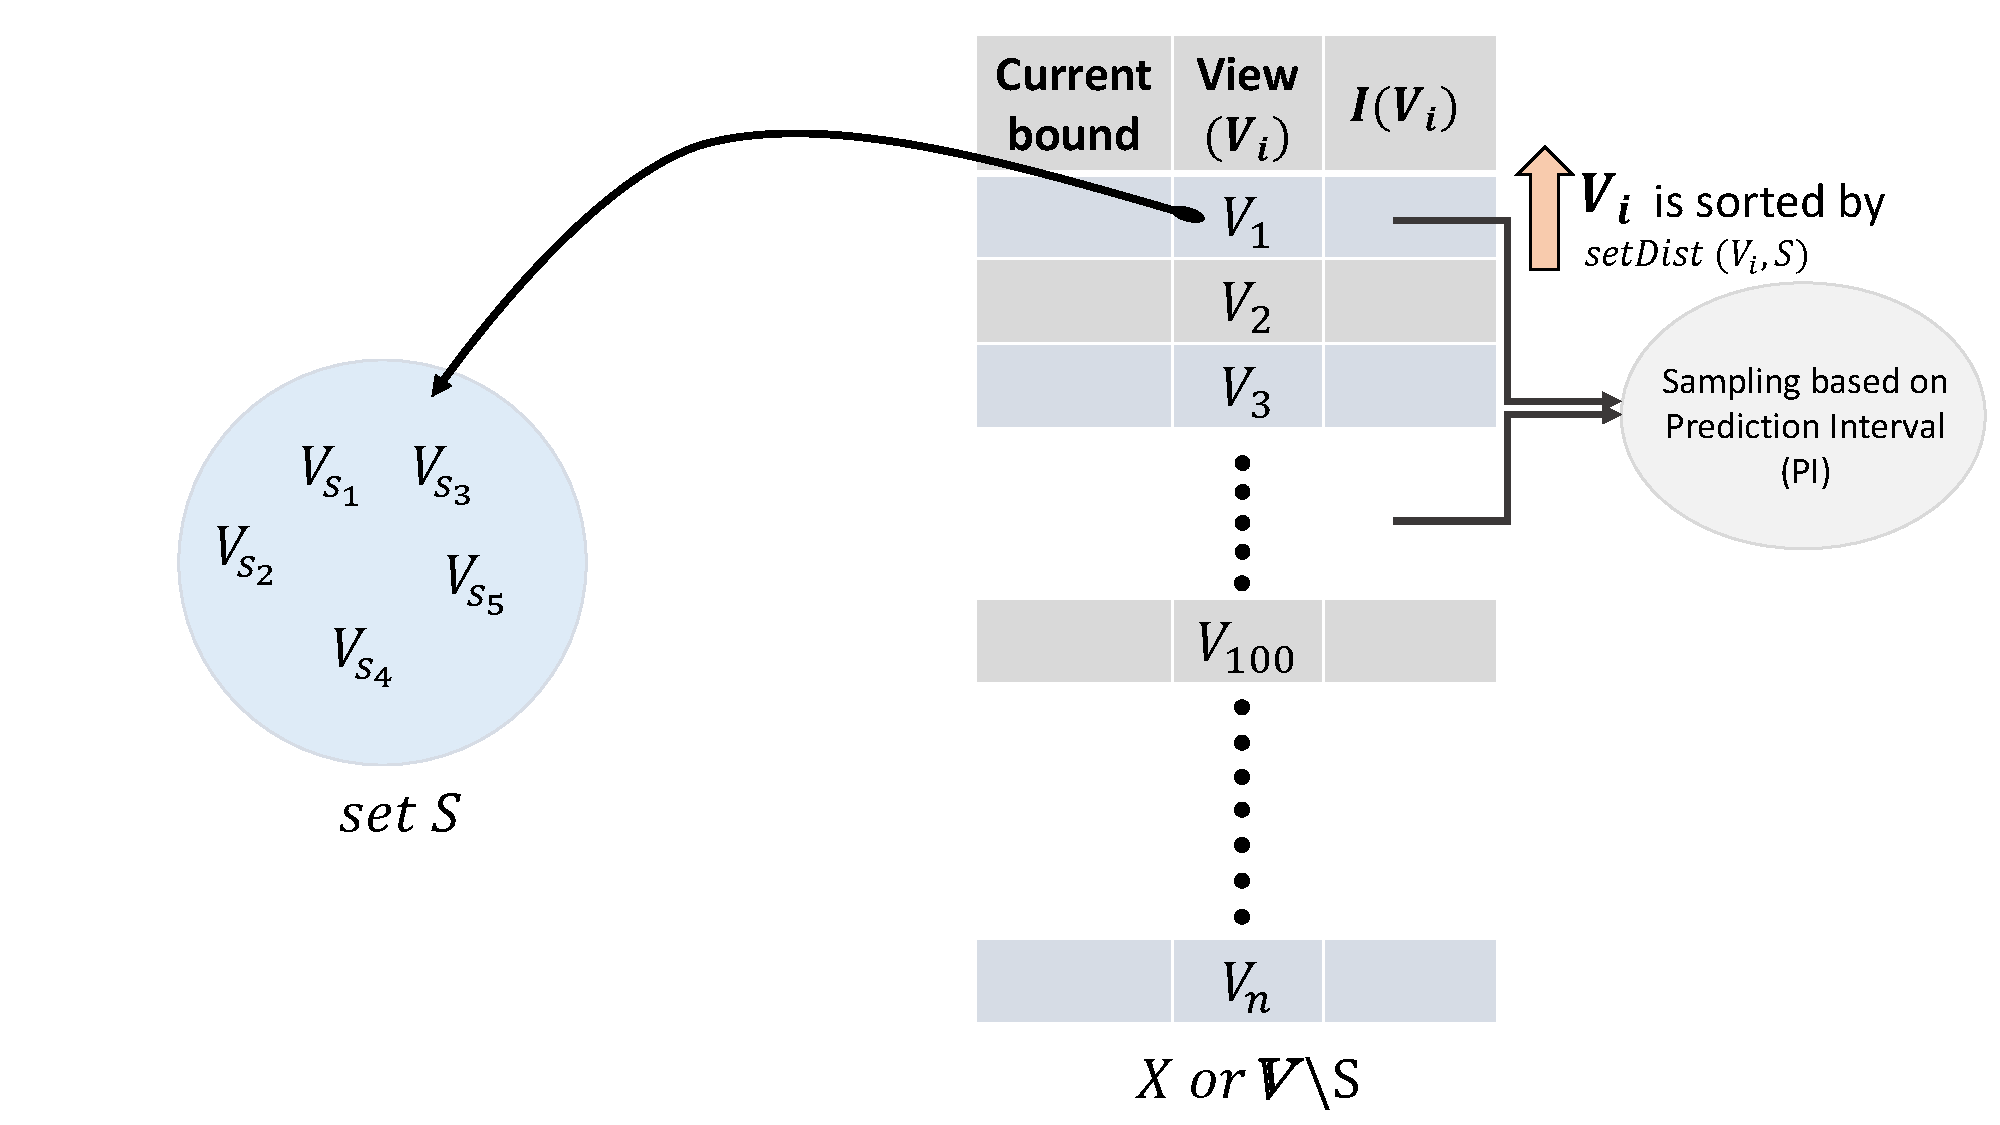
\includegraphics[width=3in]{figures/results/dSwap-Pruning}
%	\caption{dSwap-Pruning: Each candidate view has importance score and $ current bound $. The importance score of view will be generated only for view which its utility score is able to improve set $S$ while using $currentbound$ }
%	\label{fig:dSwap-Pruning}
%\end{figure}

%The idea behind pruning scheme is to minimize the query execution, which is by early prune low quality views. There are two main parameters in pruning scheme: 1) weight of $\lambda$ and 2) the max bound value $I_u$. 

%The weight of $\lambda$ is important due to it determines the contribution of importance score and diversity score. For instance, assume that an analyst wants to get set of views from view recommendation and she uses $\lambda$ = 0.7. The $\lambda$ value equal to 0.7 means that the diversity contribution to the utility score is 70\% and the contribution of importance score will be 30 \%, as it can be seen in equation \ref{objectif_function}. Thus, by setting the $\lambda$ to higher value, the contribution of importance score will be lower and more queries are pruned. This $\lambda$ value is determined by analyst, however, in this experiement 0.5 is used as the default. 
\vspace{-3pt}
% ============================================== %
% EXPERIMENTAL EVALUATION %
% ============================================== %

\section{Experimental Evaluation}\label{sec:experimental_testbed}

%In this section, we present our settings for evaluating the performance of our proposed {\em DiVE} scheme in terms of both efficiency and effectiveness. 
%
Table \ref{tab:tab-parameter} summarizes the different parameters used in our evaluation (default values are in bold).  
%
%All experiments were run on a single machine with 16 GB RAM and a 64 bit, Intel Core i7-7700 processor. 
We have conducted our experiments over the following datasets: 1) Heart Disease Dataset \footnote{http://archive.ics.uci.edu/ml/datasets/heart+Disease}: This dataset is comprised of $9$ dimensional attributes and $5$ measure attributes, resulting in a total of 180 possible views, and 2) Airline (Flights) Dataset \footnote{http://stat-computing.org/dataexpo/2009/the-data.html}: This dataset is comprised of $7$ dimensional attributes and $4$ measure attributes for a total of 112 views. While its dimensionality is lower than than the heart disease data, it is a relatively large dataset of almost one million tuples, which helps in evaluating the incurred query processing time.
%
For each experiment, the performance measures are averaged over a query workload of ten random queries submitted to select ten different subsets of data $D_Q$. 
%


\begin{table}[t]
	\caption{Parameters testbed in the experiments}
	\vspace{-10pt}
	\label{tab:tab-parameter}
	\begin{tabular}{ccl}
		\toprule
		Parameter &Range (\textbf{default})\\
		\midrule\
		datasets & \textbf{Heart disease}, Flights\\
%		sample queries & \textbf{10} \\
		diversity weight ratio & \textbf{3($ A $) : 2($ M $) : 1($ F $)} \\
		tradeoff weight $ \lambda $ & 0.0, 0.2, 0.4, \textbf{0.5}, 0.6, 0.8, 1.0 \\
		result set (size of \textit{k}) & \textbf{5}, 15, 25, 35\\
		prediction interval \% & 80 , 85, 90, 95, \textbf{97}, 98\\
	%	aggregate functions & Max Min Avg Sum \\
		%		algorithms & Linear-Importance, Greedy-Diversity, DiVE-Greedy, DiVE-Greedy-Static\\
		\bottomrule
	\end{tabular}
		\vspace{-2pt}
\end{table}



\eat{
We evaluate the performance of following schemes: 1) Linear-Importance and Greedy-Diversity, which are our baseline methods (Sec.~\ref{subsec:baseline}), 2) DiVE-Greedy (Sec.~\ref{subsec:dive-greedy}), 3) DiVE-iSwap and DiVE-dSwap (Sec.~\ref{subsec:dive-swap}), which employ an interchange algorithm initialized with the most important and most diverse views, respectively, 4) DiVE-Greedy-Static and DiVE-dSwap-Static (Sec.~\ref{dive-greedy-static} and \ref{subsec:dive-dswap}), which use static pruning techniques based on the theoretical $I_u$ (Sec.~\ref{subsec:problem_definition}), and 5) DiVE-Greedy-Adaptive and DiVE-dSwap-Adaptive, which use adaptive pruning based on predictive intervals to estimate $\bar{I}_{au}$ (Sec.~\ref{subsec:adaptive-pruning}). 
}

\eat{
\setlength{\leftmargini}{6pt}
\begin{itemize}
	\item Linear-Importance and Greedy-Diversity: Recommends top-k views on the basis of only importance, and diversity, respectively.
	\item DiVE-Greedy: Recommends top-k views on the basis of hybrid objective function using greedy algorithm.
	\item DiVE-iSwap: Selects top-k views using swap algorithm initialized by Linear-importance method. 
	\item DiVE-dSwap: Selects top-k views on the basis of hybrid objective function using swap algorithm initialized by Greedy-Diversity method.
	\item Static-pruning: DiVE-Greedy and DiVE-dSwap methods using static pruning technique to reduce the number of view queries as presented in section \ref{dive-greedy-static}  and \ref{subsec:dive-dswap}
	\item Adaptive-pruning: DiVE-Greedy and DiVE-dSwap methods using adaptive pruning method as discussed in section \ref{subsec:adaptive-pruning}.	
\end{itemize}
}

%
%In particular, the performance of each scheme listed above is measured based on the following metrics: 1) {\bf  Recommendation Quality:} measured as the value of hybrid objective function $F\left(S\right)$, and 2) {\bf Recommendation Cost:} measured as the sum of the cost to execute view queries and the cost to diversify the views that is: $C_T= C_Q + C_D$.

\eat{
\begin{figure}[t]
	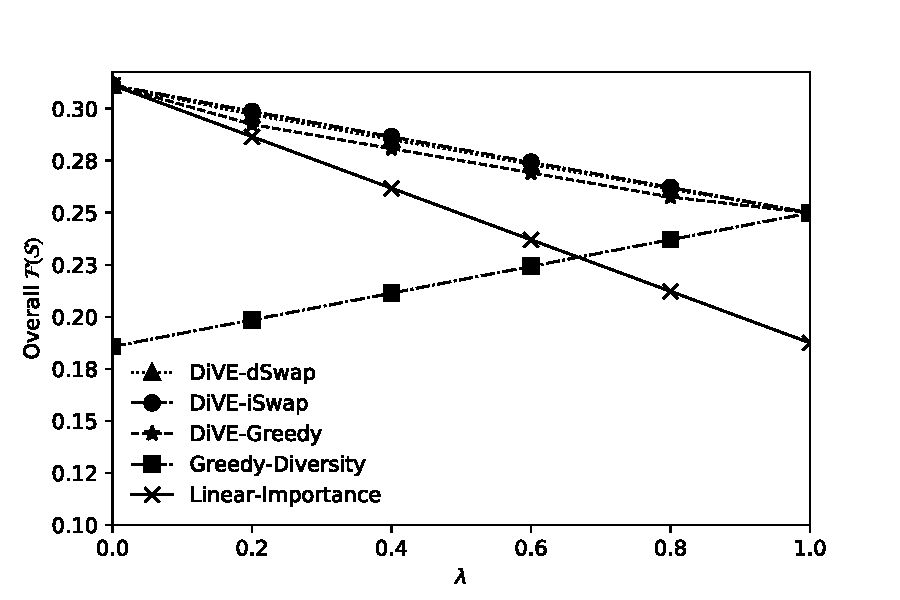
\includegraphics[width=2.6in]{figures/results/tradeoff_heart_2}
			\vspace{-15pt}
	\caption{Flights dataset}%, k = 5}
	\label{fig:impact_lambda_to_PI_sampling_greedy_pruning}
\end{figure}
}

\begin{figure}[t]
	\centering
	\subcaptionbox{Heart disease dataset}[.75\linewidth][c]{%
		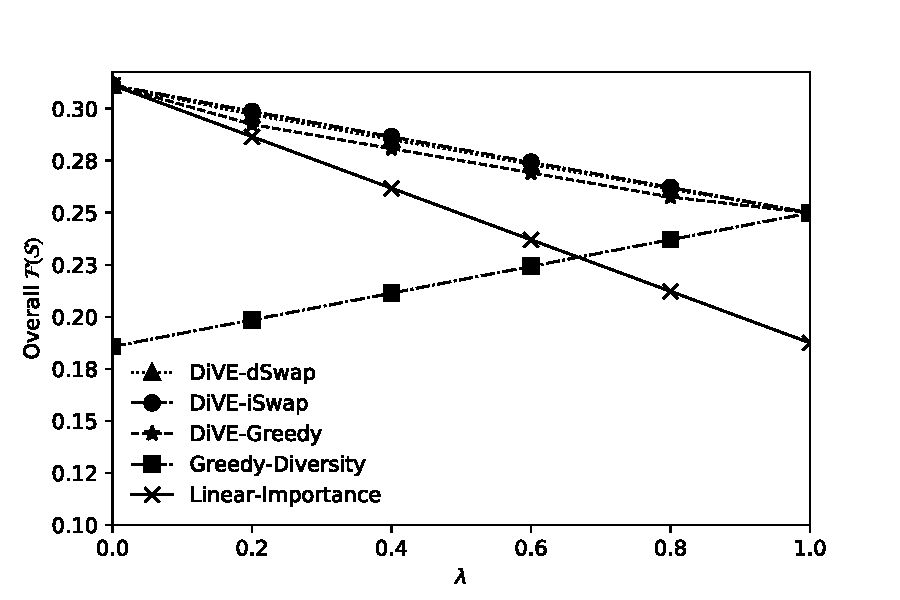
\includegraphics[width=.75\linewidth]{figures/results/tradeoff_heart_2}} \\
		\subcaptionbox{Flights dataset}[.75\linewidth][c]{%
		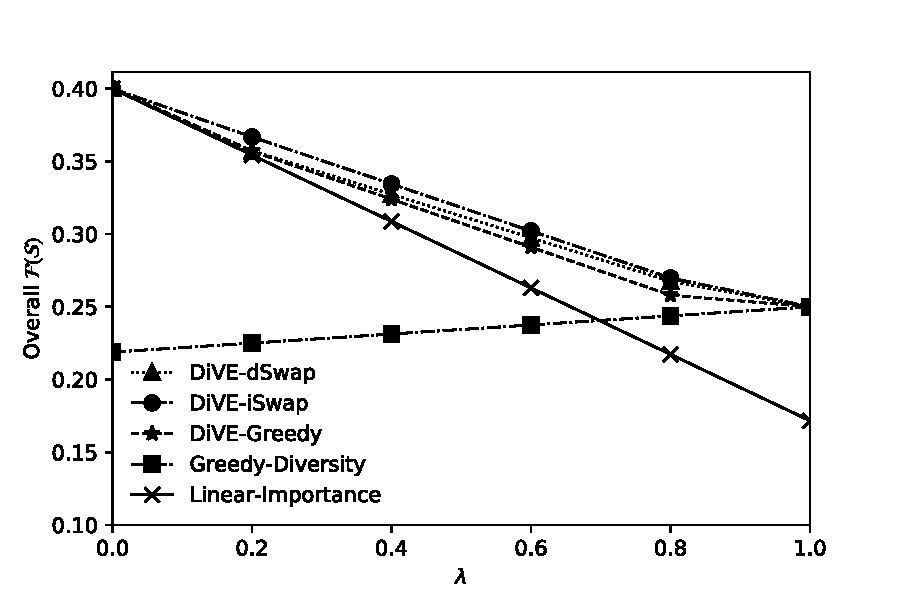
\includegraphics[width=.75\linewidth]{figures/results/tradeoff_flights}}
										\vspace{-10pt}				
	\caption{Impact of $\lambda$ on $F\left(S\right)$, k = 5}
	\label{fig:tradeoff_3_datasets}	
	\end{figure}



% The Impact of \lambda to the overall objective function value %


%\section{Experimental Evaluation}\label{sec:experimental_evaluation}

{\noindent{\bf The impact of $\lambda$ on $F$}:}
%The value of $\lambda$ balances the trade off between importance and diversity score. 
Figure \ref{fig:tradeoff_3_datasets} shows how the performance of each scheme in terms of $F\left(S\right)$ is effected as the value of  $\lambda$ varies from $0$ to $1$. Clearly, for the lower values of $\lambda$, the highest $F(S)$ is achieved by Linear-Importance. To the contrary, the Greedy-Diversity method achieves highest values of $F\left(S\right)$ as the $\lambda$ approaches $1$. 
Hence, there is a crossover between the two schemes. 
However, our proposed DiVE schemes have stable performance for all values of $\lambda$ and outperforms Linear-Importance and Greedy-Diversity. 


% The Impact of k to the overall objective function value %
{\noindent{\bf The impact of k on $F$}:} 
Figure \ref{fig:objf_3_datasets} shows the $F\left(S\right)$ values for various schemes as the number of recommended views $k$ varies from $5$ to $35$. 
%
Overall the $F\left(S\right)$ value decreases with increasing value of $k$ for all the schemes. 
%
This is because both average importance score and diversity of a set $S$ decreases as new views are added to $S$. 
%
%The views added earlier to $S$ have higher importance score then the views added later. Similarly, the diversity function exhibits a diminishing marginal gain trend as the size of set $S$ increases. 
The important observation here is the fact that our {\em DiVE} schemes always have higher overall objective function values as compared to the two extreme baselines approaches for all values of $k$. 
%Among the {\em DiVE} schemes, DiVE-iSwap and DiVE-dSwap perform better than the Greedy versions. This is because, swap algorithm performs number of additional iterations to improve the value of the objective function.

\begin{figure}[t]
	\centering
	\subcaptionbox{Heart disease dataset}[.75\linewidth][c]{%
		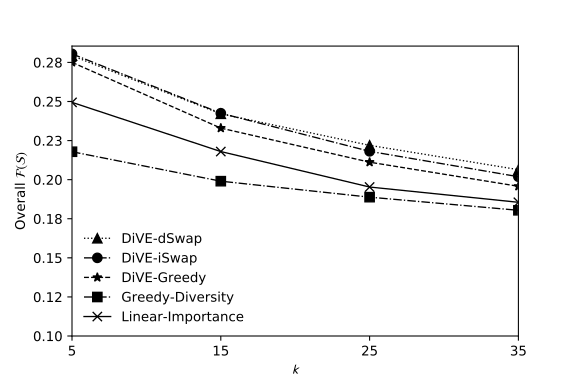
\includegraphics[width=.75\linewidth]{figures/results/objf_heart_2}} \\ 
	\subcaptionbox{Flights datasets}[.75\linewidth][c]{%
		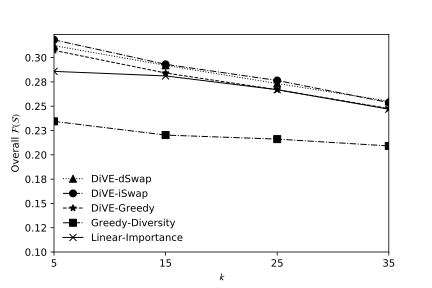
\includegraphics[width=.75\linewidth]{figures/results/objf_flights}}
								\vspace{-10pt}				
	\caption{Impact of k on $F\left(S\right)$, $\lambda = 0.5$}
	\label{fig:objf_3_datasets}
\end{figure}



%
%\begin{itemize}
%	\item Heart Disease Dataset \footnote{http://archive.ics.uci.edu/ml/datasets/heart+Disease}: This dataset is comprised of $9$ dimensional attributes and $5$ measure attributes. The number of possible views are $180$ with four aggregate functions.% and  has 14 attributes in total which are 9 attributes $ \mathbb{A} $ and 5 measure attributes $ \mathbb{M} $, $ \mathbb{A}  $= sex, cp, fbs, restecg, exang, slope, ca, thal, num; $ \mathbb{M} $ = age, trestbps, chol, thalach, oldpeak. This dataset has small number of rows (299 rows).
%	\item Airline (Flights) Dataset \footnote{http://stat-computing.org/dataexpo/2009/the-data.html}: This dataset is comprised of $7$ dimensional attributes and $4$ measure attributes. The number of possible views are $112$.%The detail as follows: $ \mathbb{A}  $= year, month, week, day, carrier, origin, destination; $ \mathbb{M}  $= arrivaldelay, departurdelay, weatherdelay, distance. This dataset has 855,632 number of rows. 
%\end{itemize}
%
%In particular, we evaluate the performance of following schemes:
%\begin{itemize}
%	\item Linear-Importance: Selects top-k views on the basis of only the importance score.
%	\item Greedy-Diversity: Selects top-k diverse views.
%	\item DiVE-Greedy: Selects top-k views on the basis of hybrid objective function using greedy algorithm.
%	\item DiVE-iSwap: Selects top-k views on the basis of hybrid objective function using swap algorithm initialized by Linear-importance method. 
%	\item DiVE-dSwap: Selects top-k views on the basis of hybrid objective function using swap algorithm initialized by Greedy-Diversity method.
%	\item Static-pruning: DiVE-Greedy and DiVE-dSwap methods using static pruning technique to reduce the number of view queries as presented in section \ref{dive-greedy-static}  and \ref{subsec:dive-dswap}
%	\item Adaptive-pruning: DiVE-Greedy and DiVE-dSwap methods using adaptive pruning method as discussed in section \ref{subsec:adaptive-pruning}.	
%\end{itemize}
%For each experiment a query workload of ten random queries is submitted to select ten different subsets of data $D_Q$. The performance measures are averaged over views recommended for each of those ten subsets. In particular, the performance of each scheme listed above is measured based on the following metrics:
%\begin{itemize}
%	\item {\bf  Interestingness of the views:} measured as the value of hybrid objective function 
%	$F\left(S\right)$ for selected set of views $S$, as defined in equation \ref{objectif_function}.
%	\item {\bf Total Cost:} measured as the sum of the cost to execute view queries and the cost to diversify the views that is : $C_T= C_Q + C_D$
%\end{itemize}


%\eat{
%	\textbf{\textit{Experimental Setup}}. This experiment running on Windows 10 64 bit, Intel Core i7-7700 CPU @ 3.60 GHz, RAM 16 GB. The experiment is developed using Python and run on Python version 3.6.3 with PostgreSQL as the database engine. Two real datasets are used, as follows: 
%}
%
%\eat{
%	\subsection{Effectiveness Evaluation}
%	%  Prolog of the quality of the results evaluation%
%	In order to test the performance of our proposed approach, we run experiments using two real datasets: flights dataset and heart disease dataset. For each dataset, we execute ten random queries. Afterwards, the average of all results is calculated as the final result. We examine the performance of our proposed schemes in term of the quality of the result (effectiveness) and the efficiency. All parameters used in this experiments are summarized in Table \ref{tab:tab-parameter} and the detail results of the experiments is elaborated next. 
%}
%\subsection{Efficiency and Pruning Scheme Evaluation}
\begin{figure}[t]
	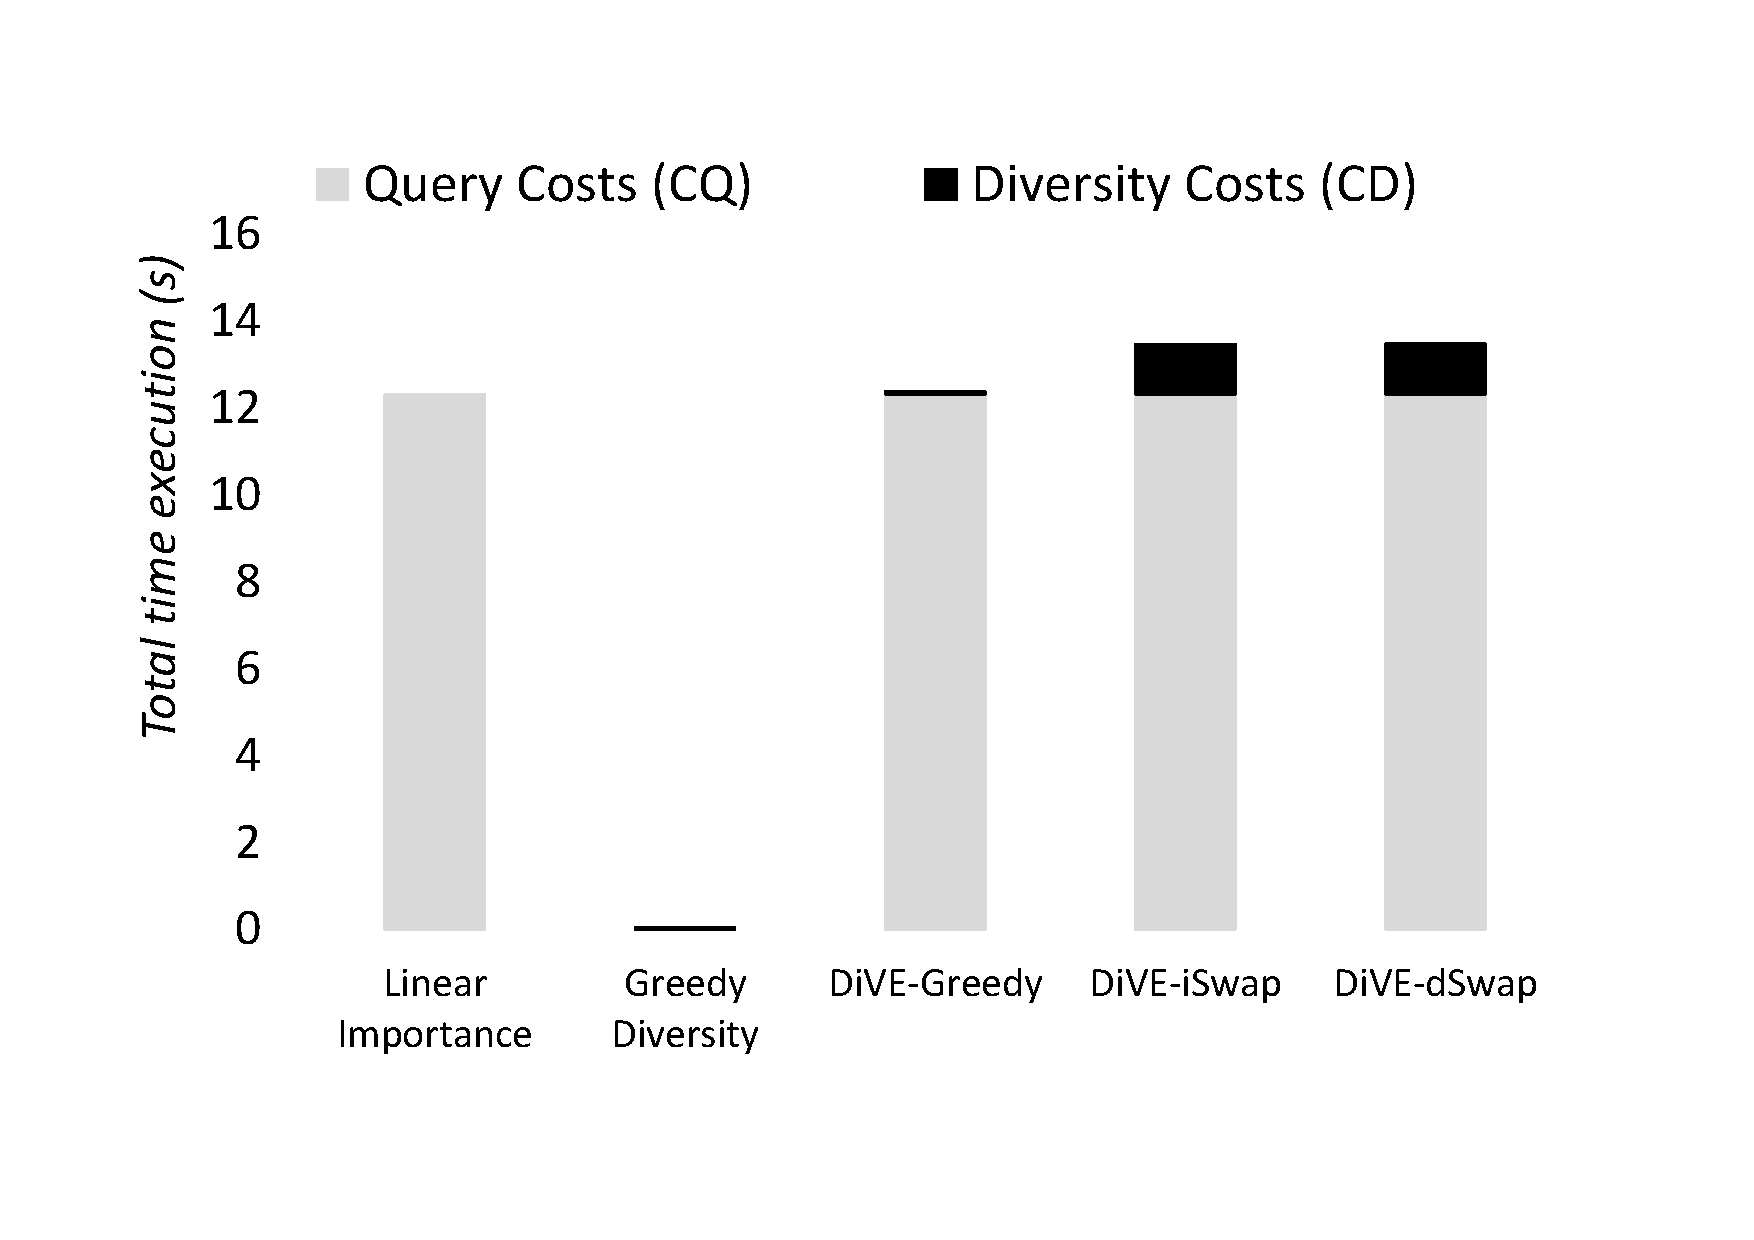
\includegraphics[width=2.6in]{figures/results/flight_costs}
		\vspace{-15pt}
	\caption{Cost Analysis of DiVE, k =5, $\lambda = 0.5$}
	\label{fig:cost_flights}
		%\vspace{-5pt}
\end{figure}
% Efficiency and Pruning Scheme%

% Overall execution time / Overall costs to run all schemes%

{\noindent{\bf Execution time evaluation}}
In this experiment we measure the cost of {\em DiVE} in terms of execution time. Figure \ref{fig:cost_flights} plots the execution time for Flights dataset with $k = 5$ and $\lambda = 0.5$. The total execution time is split into the query execution time $C_Q$ and the diversification cost $C_D$. It is clear from Figure \ref{fig:cost_flights} that the total execution time $C_T$ is dominated by the cost of generating the views $C_Q$. Hence, the minimum cost is incurred by the Greedy-Diversity method which only computes diversity. For all other methods, the $C_Q$ component of the execution time is same as all views are generated only once. However, the cost of diversification $C_D$ is slightly higher for DiVE-iSwap and DiVE-dSwap as compared to the DiVE-Greedy due the higher number of iterations. 





%\subsubsection{Static-Pruning scheme performance}


% Impact of lambda (parameter to tradeoff between importance and diversity) to the pruned queries, running on Heart disease dataset %
%

\begin{figure}[t]
	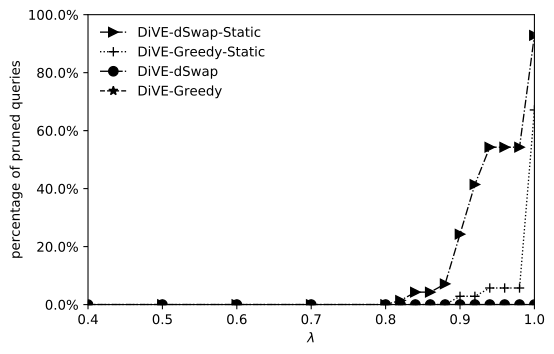
\includegraphics[width=2.6in]{figures/results/no_pruning_vs_static}
			\vspace{-15pt}
	\caption{Impact of Static pruning}%, k = 5}
	\label{fig:impact_lambda_to_PI_sampling_greedy_pruning}
		%\vspace{-6pt}
\end{figure}


{\noindent{\bf Impact of static Pruning}}
In this experiment we present the performance of our proposed pruning techniques in terms of the number of pruned queries required to generate the views. The higher number of pruned queries result in the higher cost savings in the total query execution time. Figure \ref{fig:impact_lambda_to_PI_sampling_greedy_pruning} shows the performance of our static pruning technique using the maximum value of importance score $I_u$. In this and next experiments, DiVE-iSwap is not evaluated as it executes all the view queries for the initial set selection and any pruning afterwards is not possible. Moreover, due to space limit, we use only the heart disease dataset in the next experiments.

For both schemes DiVE-Greedy-Static and DiVE-dSwap-Static, since the $I_u$ value can be far from the actual importance scores of individual views, the percentage of pruned queries is $0$ for lower values of $\lambda$. Only for $\lambda$ close to $0.9$ some queries get pruned. DiVE-dSwap-Static  is able to prune higher number of queries than DiVE-Greedy-Static. At $\lambda=1$, DiVE-dSwap-Static prunes $80\%$ queries while DiVE-Greedy-Static prunes almost $65\%$ queries. 

%This is because for $\lambda = 1$ the weight of importance score is $0$ in the hybrid objective function and the overall value of $F\left(S\right)$ is determined by the diversity score only.

\begin{figure}[t]
	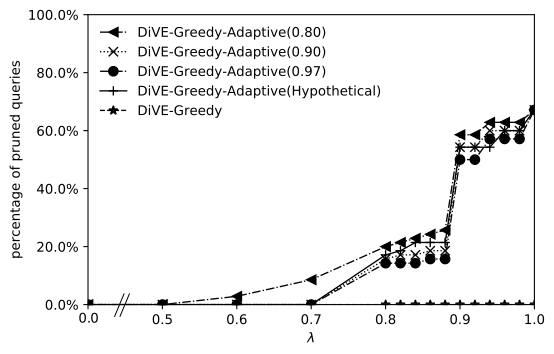
\includegraphics[width=2.6in]{figures/results/pruning_performance_greedy_adaptive}
			\vspace{-15pt}
	\caption{DiVE-Greedy with Adaptive Pruning}%, k = 5, $\lambda = 0.5$}
	\label{fig:pruning_performance_greedy}
		%\vspace{-6pt}
\end{figure}

\begin{figure}[t]
	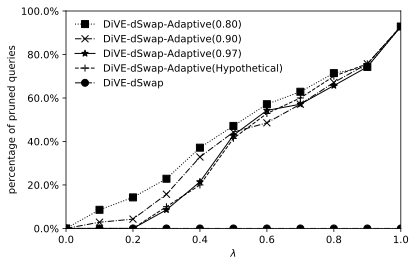
\includegraphics[width=2.6in]{figures/results/pruning_performance_dswap_adaptive}
				\vspace{-15pt}
	\caption{DiVE-dSwap with Adaptive Pruning}%, k = 5, $\lambda = 0.5$}
	\label{fig:impact_lambda_to_PI_sampling_swapd_pruning}
	%\vspace{-6pt}
\end{figure}



{\noindent{\bf Impact of Adaptive Pruning}}
In this experiment we analyze the performance of adaptive pruning technique under different values of $\lambda$ and prediction interval $PI$. As shown in Figure \ref{fig:pruning_performance_greedy}, DiVE-Greedy-Adaptive is able to prune queries even for lower values of $\lambda$. The number of queries pruned increase significantly for higher values of $\lambda$. In comparison to the static pruning as shown in Figure \ref{fig:impact_lambda_to_PI_sampling_greedy_pruning}, with adaptive pruning DiVE-Greedy is able to prune almost $20\%$ more queries at $\lambda = 0.8$. Figure \ref{fig:impact_lambda_to_PI_sampling_swapd_pruning} shows the performance of DiVE-dSwap-Adaptive with different values of $ PI $. In comparison to DivE-Greedy-Adaptive, the number of pruned queries by DivE-dSwap-Adaptive are much higher for all values of $\lambda$. The interesting observation is the fact that DiVE-dSwap-Adative is able to prune $15\%$ queries for $\lambda$ values as low as $0.2$. For higher values of $\lambda$ the percentage of pruned queries is between $60\%$ and $90\%$. Similar to DiVE-Greedy-Adaptive, highest number of queries are pruned for $PI=0.8$. 
	
	%The performance declines slightly as we increase $PI$ to $0.97$. This is because when the sample size is large, many queries are already executed and the margin of cost savings by pruning the remaining queries is small.
%\end{itemize}

\begin{figure}[t]
	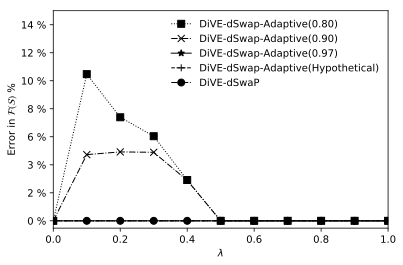
\includegraphics[width=2.6in]{figures/results/error_f_s}
				\vspace{-15pt}
	\caption{Impact of Adaptive pruning on $F(S)$}
	\label{fig:pruning_performance_swapd}
\end{figure}

Further we evaluate the effectiveness of methods with adaptive pruning in terms of the $F\left(S\right)$ values. 
%Although, adaptive pruning is based on approximation of the actual importance score bounds, still the loss in the $F\left(S\right)$ values of the computed set of views is very small. 
Figure \ref{fig:pruning_performance_swapd} shows the loss in $F\left(S\right)$ in comparison to the $F\left(S\right)$ values achieved by Hypothetical methods. The loss for both DiVE-Greedy-Adaptive and DiVE-dSwap-Adaptive is $0\%$ for $PI=0.97$, With a larger sample size the accuracy of approximated importance score is higher. For a smaller sample size of $PI=0.80$ there is 0\% loss while $\lambda = 0$ because at the moment there are no pruned queries. However, there is a maximum loss of $10\%$ at $\lambda= 0.1$. The loss in $F\left(S\right)$ values decrease as $\lambda$ increases as the impact of importance score becomes smaller in the hybrid objective function. Meanwhile, starting $\lambda \geq 0.5$ the loss is 0\%.

% it can be confirmed in Figure \ref{fig:impact_lambda_to_PI_sampling_swapd_pruning} that shows the performance of DiVE-dSwap-Adaptive($0.80$) close to DiVE-dSwap-Adaptive($0.97$) and DiVE-dSwap-Adaptive(Hypothetical) which there is no loss for both of them.


% The impact of query load to the pruning performance %
{\noindent{\bf The impact of query subset on pruning}}
The pruning power of our algorithms is effected by the maximum importance score views generated over a data subset $D_Q$ in comparison to the reference subset $D_R$. If the highest importance score of any view generated over $D_Q$ is far less than the upper bound of $\sqrt{2}$ (Sec. ~\ref{subsec:problem_definition}), then only few queries will be pruned. 
%
%Similarly, for adaptive pruning technique higher or lower importance scores of views will effect the number of pruned queries. 
%
Thus, for this experiment, we created three different clusters of heart disease subsets. And categorized them as low, medium and high. Where low dataset is the subset with low values of importance score (i.e., {\tt low importance query load}) and high is the subset with higher values of importance score (i.e., {\tt high importance query load}). We run experiments using those two type of query load and compared the performance of pruning methods in terms of number of queries pruned. The $ PI $ value is set to default value of $0.97$. It can be seen in Figure \ref{fig:low_vs_high} that both DiVE-Greedy-Adaptive and DiVE-dSwap-Adaptive perform better on low importance query load. For high importance query load less number of queries are pruned. This shows that the characteristic of the query subset $D_Q$ has an impact on the efficiency of the pruning methods.


\begin{figure}[t]
	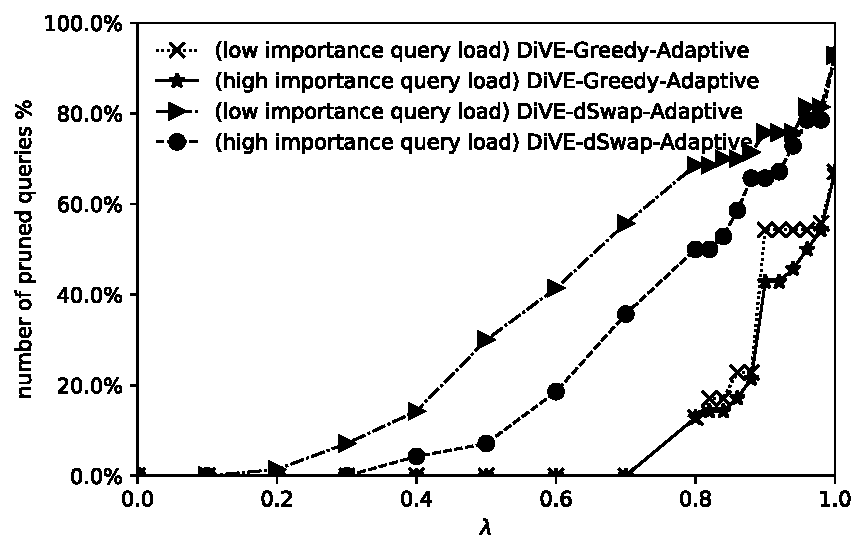
\includegraphics[ width=2.6in]{figures/results/low_vs_high_new}
			\vspace{-15pt}
	\caption{Impact of Query Subset}
	\label{fig:low_vs_high}
\end{figure}

%
%
%\eat{
%	\textbf{\textit{The total time to run DiVE schemes}}. In order to start analyzing the efficiency, we need to know the main issue in term of costs. Figure \ref{fig:cost_flights} shows the example of exactly time that needed to run schemes on flights dataset. It shows Greedy-Diversity which only considering diversity and no query executions, it has very low costs. Meanwhile, Linear-Importance and \textit{DiVE-Greedy} seems in the same line but that was not exactly same. The total of diversity computations $ C_D $ of \textit{DiVE-Greedy} is very low, the total costs of \textit{DiVE-Greedy} is dominated by query costs $ C_Q $. Due to of this reason, the total execution time of \textit{DiVE-Greedy} closes to Linear-Importance. Those are the proof that the total costs of all schemes execpt Greedy-Diversity are dominated by query cost $ C_Q $. }
%
%\eat{
%	Due to the page limitation, all our experiments in three real dataset cannot be showed. Hence, for the next sections, we use heart disease dataset as our focus observation. 
%	% Static Pruning Scheme Performance%
%}
%
%\eat{
%	\textbf{\textit{Impact of $\lambda$ to the pruned queries of \textit{DiVE-Greedy} scheme}}. In this work, we proposed two kind of pruning schemes, that are using estimated static value of maximum value of the importance score $maxI$ and using adaptive maximum value of importance score. 
%	
%	The first our pruning scheme is using static value $maxI$. To check the performance of our pruning scheme, we run it to all real datasets using different value of $ \lambda $. We analyze the result by comparing the result of schemes with pruning enable on it and the schemes without pruning enable on it. The example result which running on heart disease dataset is shown in Figure \ref{fig:pruning_performance_greedy} . The static pruning scheme only able to prune queries while the value of $\lambda$ is high, closes to 0.9. As we expected, it is because the value of $maxI$ that too far from the real value of importance score. 
%	
%	%\subsubsection{Adaptive scheme performance}
%	To overcome the flaw in static pruning scheme, we also proposed adaptive pruning scheme which used dynamic value of the maximum importance score $maxI$. In order to get $maxI$ as close as possible to the real value of importance in the dataset, we applied sampling method. By using adaptive pruning, users also able to change the confidence and the margine error to tradeoff between time and precision. 
%	
%	% Impact of lambda to the pruned queries for adaptive pruning scheme %
%	
%	\textbf{\textit{Impact of $\lambda$ to the pruned queries of \textit{DiVE-dSwap} scheme}}. If static pruning scheme only able to prune queries while $\lambda$ closes to 0.9 and higher, in this section, we shows the adaptive pruning performance. Figure \ref{fig:pruning_performance_swapd} shows the performance of adaptive pruning scheme by using different value of $\lambda$. It shows the impact of $\lambda$ to the percentage of pruned queries. The adaptive pruning schemes especially \textit{DiVE-dSwap-Adaptive} is able to prune queries significantly, pruning start while $\lambda$ closes to 0.2 and by increasing the $\lambda$, more queries can be pruned.
%}
\vspace{-3pt}
% ============================================== %
% CONCLUSIONS %
% ============================================== %

\section{Conclusions}
We proposed an effective visualization recommendation scheme that integrates both importance and diversity in the recommended views. Our proposed scheme, called {\em DiVE}, combines importance and diversity into a {\em hybrid utility function} to provide full coverage of the possible insights to be discovered. In addition to employing a hybrid utility function for effective view recommendation, {\em DiVE} also leverages the properties of both the importance and diversity metrics to prune a large number of query executions without compromising the quality of recommendations. 

%Hence, providing an efficient solution for a computationally expensive view recommendation task. 

%We conducted extensive experimental evaluation on real data sets, which illustrate the benefits achieved by {\em DiVE} both in terms of effectiveness and efficiency.


%
%\eat{
%In this paper, we proposed \textit{DiVE} scheme which the main purposes are to evaluates and optimizes the results of visualization recommendation systems with respect to importance and diversity. The advantage of \textit{DiVE} is that analyst can set their preferences by changing the parameter to tradeoff between importance and diversity to get result set. We also performed an experimental study and present the results which focus on effectiveness and efficiency of our approach on real datasets. We proposed \textit{DiVE} scheme which based on Greedy and Swap approach, \textit{DiVE-iSwap} have the best performance in recommending result views but it has the highest costs due to this scheme executing all possible view from the dataset, this scheme can be used for the analyst who only cares about the results without worrying execution time. However, to the analyst who care about execution time, we proposed \textit{DiVE-dSwap-Adaptive} and \textit{DiVE-Greedy-Adaptive}, those schemes are able to decrease costs significantly without reducing the quality of results.
%%\end{document}  % This is where a 'short' article might terminate
%}

\vspace{-3pt}

%% ============================================== %
% INTRODUCTION %
% ============================================== %

\section{Introduction}

% Prolog / Background %

In the recent years, data visualization tools have become an integral part of data exploration systems. The users who are interested in finding some meaningful insights in data have neither time nor patience to manually generate all possible data visualizations. In addition to time, the domain knowledge is another key factor when generating visualizations manually. However, with an exponential growth of available data in various domains, there has been an increase in the number of \textit{Data Enthusiasts}, people with little domain knowledge and technical expertise, looking for interesting trends in data.

\begin{figure}
	\centering
	\begin{subfigure}[b]{0.40\textwidth}
		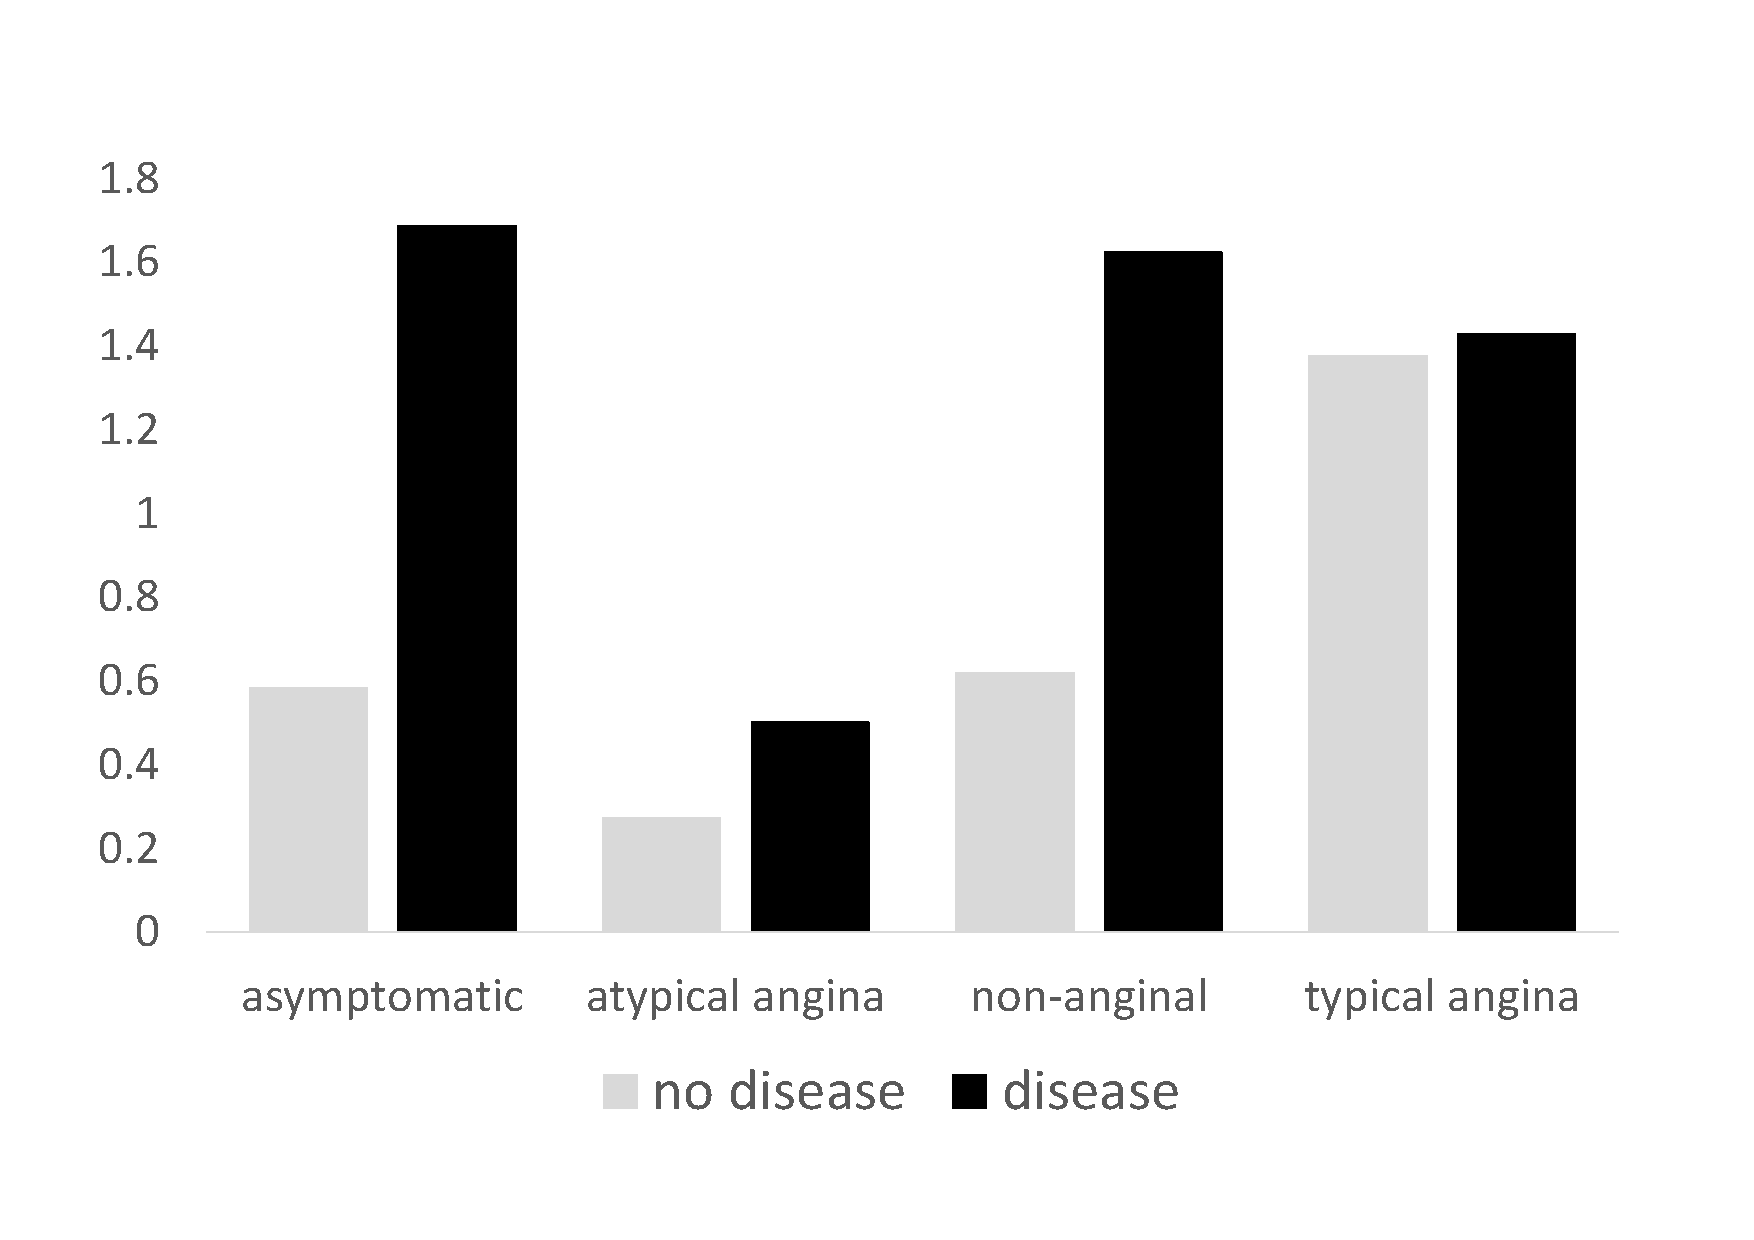
\includegraphics[width=2.5in]{figures/introduction/cp_avg_oldpeak}
		\caption{Visualization of the avg. oldpeak vs. chest pain types}
		\label{fig:intro1} 
	\end{subfigure}
	
	\begin{subfigure}[b]{0.40\textwidth}
		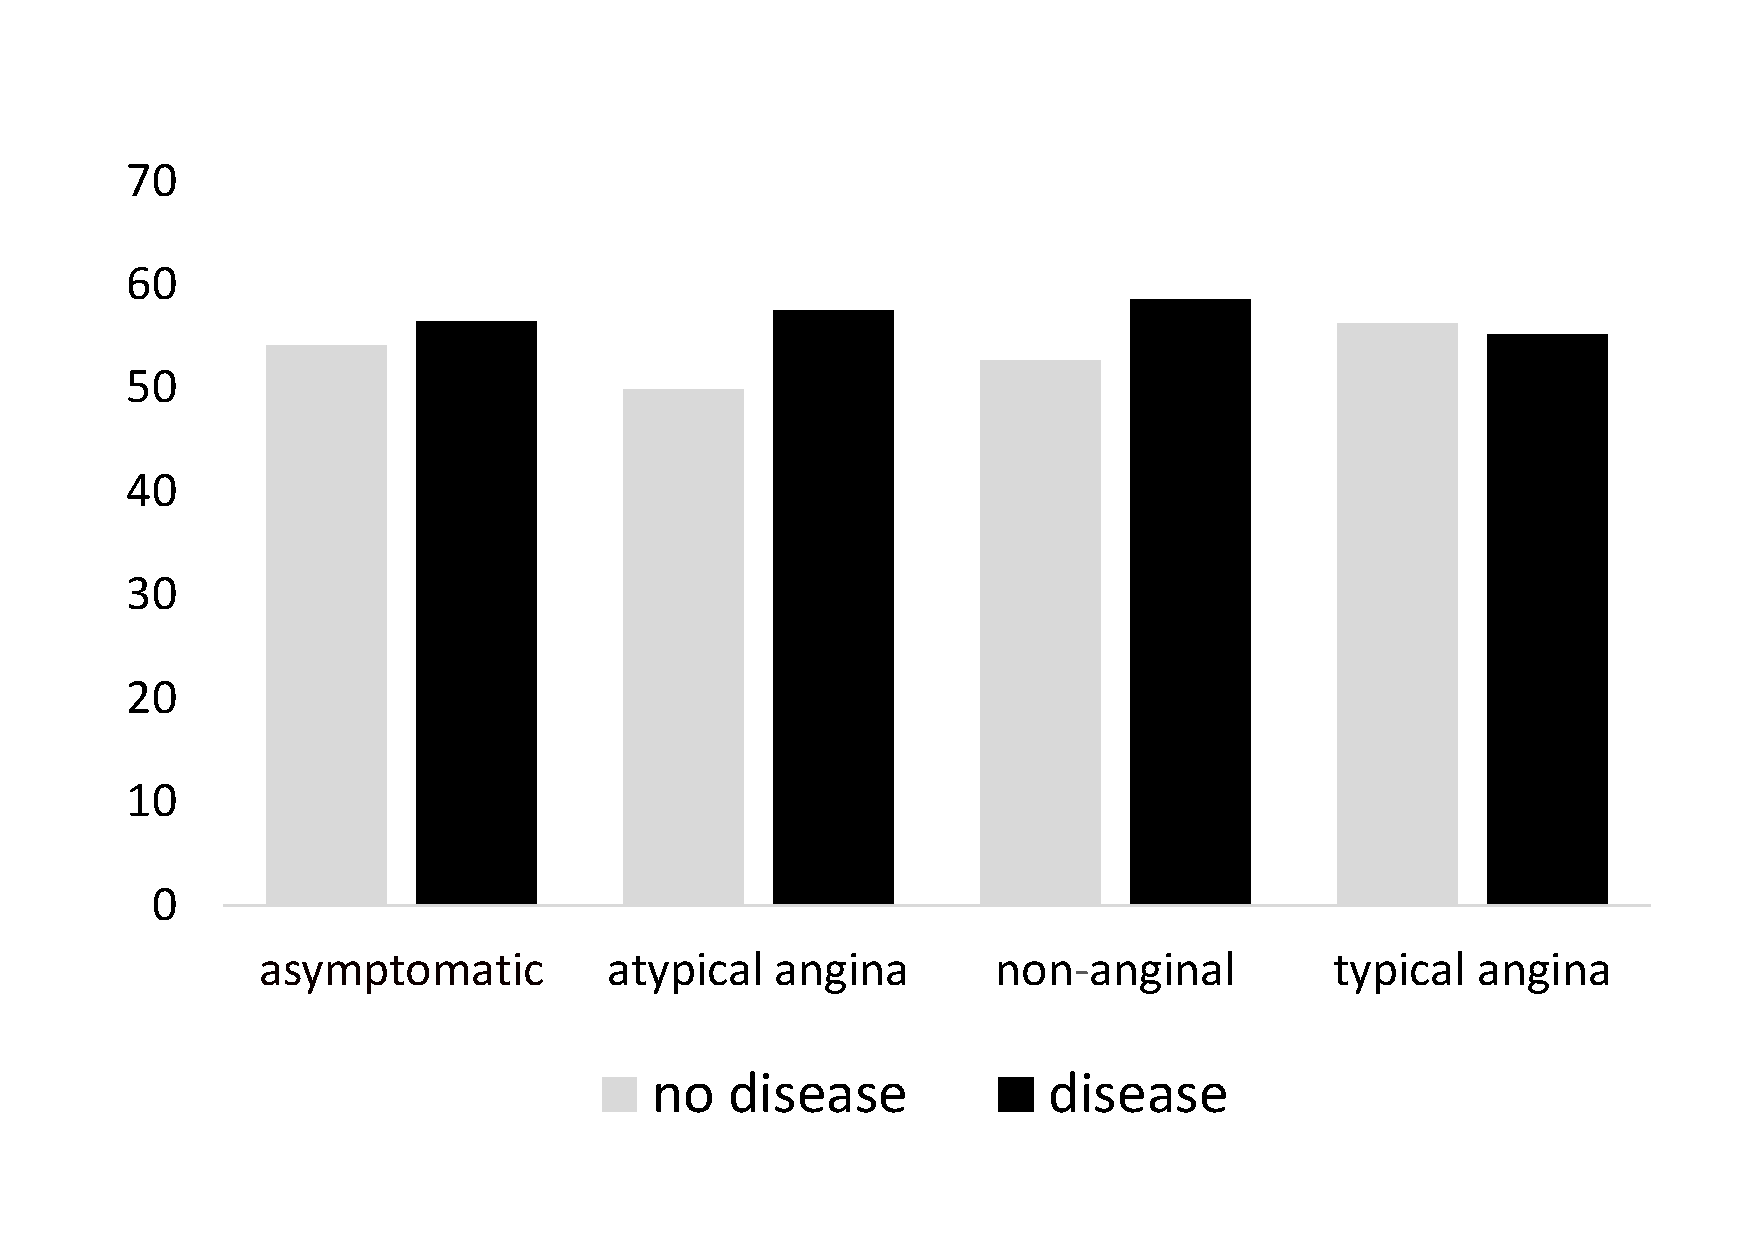
\includegraphics[width=2.5in]{figures/introduction/age_oldpeak}
		\caption{Visualization of the average age vs. chest pain types }
		\label{fig:intro2}
	\end{subfigure}
	\caption[important vs not]{Important vs. less important view.}
\end{figure}

% Example /Case %

For instance, consider a Cleveland heart disease dataset \footnote{http://archive.ics.uci.edu/ml/datasets/heart+Disease}, which describes patients with and without a heart disease.  A data enthusiast might be interested in conducting some comparison between people with heart disease (disease) and people without heart disease (no disease). Without any prior insights about data, she must manually specify different combinations of attributes, measures and aggregate functions before finally generating a visualization that reveals some interesting information about the dataset.  The user effort and time spent in that process increases exponentially with increase in the number of attributes and measures. Hence, several data-driven visualization recommendation tools have been proposed to reduce the user effort and time during data exploration \cite{Vartak2014, Vartak2015, Ehsan2016}. The main goal of those recommendation systems is to provide the user with the most important visualizations (top-k views), which are selected from all possible visualizations. The top-k views are selected based on the most important views in the dataset. The importance of a view is defined on the basis of particular criteria. One of the widely used criteria for importance is based on the deviation between the queried subset of data (target view) with the reference subset of data (reference view). The reference subset can be another subset of the dataset, the rest of the dataset, or the whole dataset. The intuition behind deviation based approach is that views that reveal substantially different trends from the reference views are likely to be of higher interest to the user\cite{Vartak2014, Vartak2015}.  

% Explanation of the example %

Consider again the example of the heart disease dataset. Let the target subset be the data of people with heart disease and the reference subset be the data of people without heart disease. As shown in Figure \ref{fig:intro1} the average oldpeak (pressure of the ST segment) vs. chest pain types is more important view rather than the Figure \ref{fig:intro2} the average of age vs. chest pain types, due to the large deviation between target view (disease) and reference view (no disease) data. Figure \ref{fig:intro1} shows people with heart disease, especially who the chest pain types is asymptomatic tend to have much higher oldpeak rather than people without disease. To the contrary, the Figure \ref{fig:intro2} is potentially less important visualization compared to Figure \ref{fig:intro1}, even there is a deviation between disease and no disease but the deviation is very small and if it is compared to Figure \ref{fig:intro1}, it has lower deviation than Figure \ref{fig:intro1}. Figure \ref{fig:intro2} shows that there is no significant different in term of the average age of the people with four types of chest pain.
\begin{figure}
	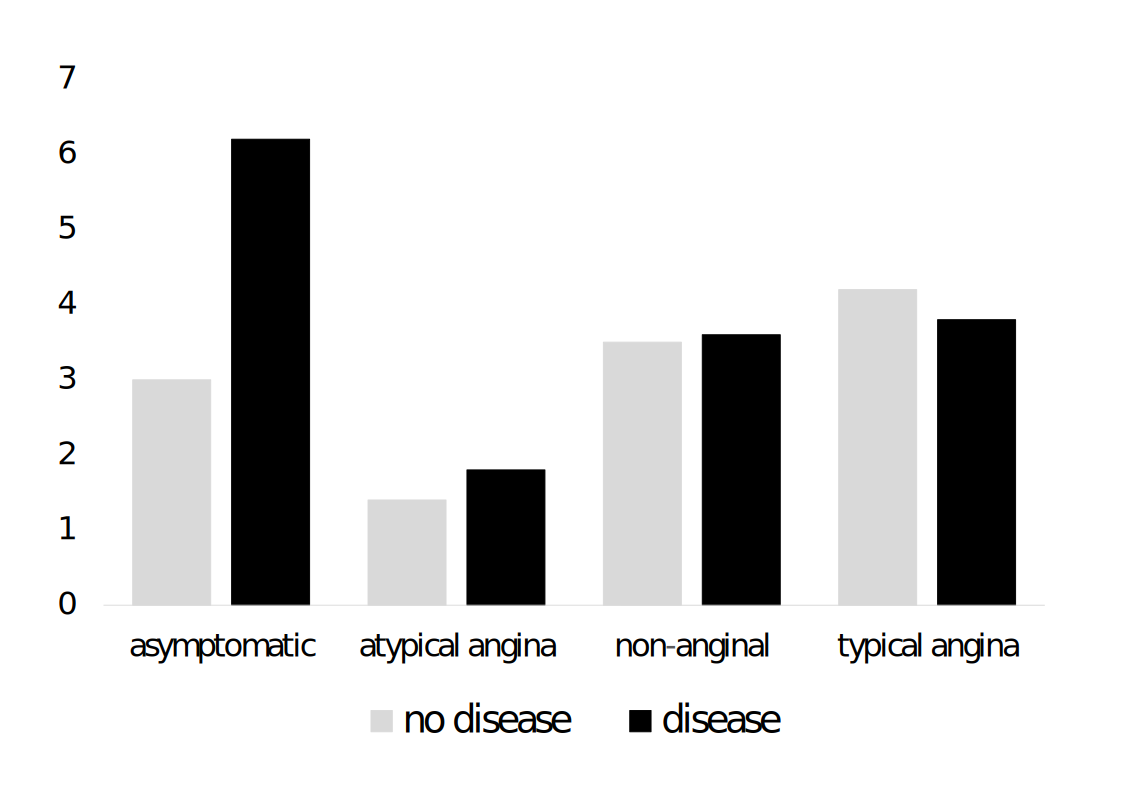
\includegraphics[width=2.5in]{figures/introduction/cp_max_oldpeak}
	\caption{The visualization of maximum oldpeak vs. chest pain types}
	\label{fig:intro3}
\end{figure}

% Problem/Issue in the current solution %

Although the deviation based visualization recommendation systems automatically provide users with the most important visualizations, it is likely that the views in the top-k set might be providing redundant information. For instance, Figure \ref{fig:intro3} provides the information which close to Figure \ref{fig:intro1} that the people with heart disease tend to have higher oldpeak values. Figure \ref{fig:intro3} has same attribute and attribute measure to Figure \ref{fig:intro1}, the only difference is the aggregate function, where Figure \ref{fig:intro1} uses AVG and Figure \ref{fig:intro3} uses MAX. Since both views have a high deviation from the reference subset, both will appear in the top-k set. This leads to an important observation that using only importance as the selection criteria may deliver redundant recommended views, which leads to presents not optimal insights. 

% Proposing Solution %
However, novelty and diversity are one of the fundamental characteristics of any effective recommendation systems \cite{Zhang2008,Clarke2008,Rafiei2010, Yu2009}. Specifically, it is highly desirable that a visualization recommendation systems provides users with views that are both importance and also provide novel information that has not been revealed by the other views. 

% Lists of contributions %
Towards designing an effective visualization recommendation systems that promotes both importance and novelty in recommended views, in this work, we propose an integrated approach called \textit{i-DiVE}. In particular, \textit{i-DiVE} aims to generate top-k visualizations that balance the tradeoff between importance and diversity. The main contributions of this paper are summarized as follows:

\begin{itemize}
	\item We formulate the problem of evaluating recommended views that are both importance and diverse. 
	\item We define a similarity measure to capture the distance between two visualizations.
	\item We present a hybrid objective function to balance the tradeoff between importance and diversity when ranking the visualizations.
	\item We propose the novel \textit{i-DiVE} scheme, that employs various algorithms to evaluate the recommended visualizations based on the hybrid ranking/objective function.
	\item We present optimization techniques that leverage the hybrid objective function to substantially reduce the computational costs.
	\item We conduct an extensive experimental evaluation on real datasets, which compare the performance of various algorithms and illustrate the benefits achieved by \textit{i-DiVE} both in terms of effectiveness and efficiency. 
\end{itemize}


The rest of the paper is organized as follows: in Section II, we formulate the top-k diverse visualization problems and our related work; we present our proposed scheme \textit{i-DiVE}  in Section III; the experimental evaluation is reported in in Section IV and we conclude in Section V.








% ============================================== %
% PRELIMINARIES %
% ============================================== %

\section{PRELIMINARIES AND RELATED WORK}
\subsection{Visualization Recommendation Systems}

% Visualization Recommendation System explanation %

In this work, we consider a visual data exploration session that begins by an analyst submitting a query $Q$ on a multi-dimensional database $D_B$ to be visually analyzed. We assume that the analyst desires to select a subset of $D_B$  by specifying a query predicate $T$. Hence, a general format for query $Q$ can be defined as: 

\bigskip
$Q$ = SELECT * FROM $D_B$ WHERE $T$;
\bigskip

The result of $Q$ is $D_Q$ which is a subset of $D_B$ that need to be visualized.

In order to generate visualizations for $D_Q$, the $D_B$ consists of a set of dimensional attributes $\mathbb{A}$ and a set of measure attributes $\mathbb{M}$. Also, let $\mathbb{F}$ be a set of possible aggregate functions over measure attributes, such as COUNT, AVG, SUM, MIN and MAX. Using different combinations of dimension and measure attributes along with various aggregate functions, and specifying GROUP BY, it is possible to execute aggregate queries over $D_Q$.  %Each aggregate query generates a two column result, where column one consists of attribute dimension values and second column presents the corresponding aggregate function values on measure attribute.
The result generated by the aggregate query can be easily visualized as bar charts. 

For instance, consider again example 1. Let $D_B$ be Cleveland heart disease data table (e.g., tb\_heart\_disease). The analyst wants to do comparison between people with heart disease (disease) and people without heart disease (no disease). This example leads us to the two subsets which are disease subset as the target subset $D_T$ and no disease subset as the reference subset $D_R$.
Hence, each of the subset, leads to a unique visualization called a target view denoted as $V_T$ and a reference view denoted as $V_R$. We can formally define as: 

\bigskip
$V_T$  = SELECT $A$, $F$ ($M$) FROM $D_B$ WHERE $T_T$ GROUP BY $A$;

$V_R$  = SELECT $A$, $F$ ($M$) FROM $D_B$ WHERE $T_R$ GROUP BY $A$;
\bigskip

where $A \in \mathbb{A}$, $M\in \mathbb{M}$, and  $F \in \mathbb{F}$. We consider the attribute and measure dimensions of $D_B$ which are; $\mathbb{A}$ =  (chest\_pain\_types), $\mathbb{M}$ = (age, oldpeak) and $\mathbb{F}$ = (COUNT, AVG, SUM, MIN and MAX). The query predicate $T_T$ is \quotes{status = Disease}, this predicate generates a subset $D_T$ of $D_B$ that contains data of all patients with heart disease. Meanwhile, the query predicate $T_R$ is \quotes{status = No Disease} which generate subset $D_R$ of $D_B$ and it consists the data of all patients without heart disease. Using various combinations of attributes, measures and aggregate functions, it is possible to generate 2 * | $\mathbb{A}$ |*| $\mathbb{M}$ |*| $\mathbb{F}$ | = 2*(1*2*5) = 20 views. For instance, the views shown in Figure \ref{fig:intro1} and \ref{fig:intro2} correspond to $A$=\quotes{chest\_pain\_types}, $M$=\quotes{age}, \quotes{oldpeak}, and $F$=\quotes{Avg}. In addition, the view of Figure \ref{fig:intro3}  corresponds to $A$=\quotes{chest\_pain\_types}, $M$=\quotes{oldpeak}, and $F$=\quotes{Max}.

It is clear from the above example that even for a modest dataset that only has one attribute and two meassure attributes, the number of possible views to consider can be large. Also, not all the views will be of interest to the user. Therefore, in order to reduce the user effort, it is very important to recommend a set of few \quotes{most important} views. The challenge, however, is to determine what constitutes the most imporant of set of views. Most of the existing visualization recommendation systems techniques rely mainly on the content of the view in terms of data generated as a result of the underlying aggregate query\cite{Vartak2015}, \cite{Vartak2014}. Those exiting approaches lead to recommend homogeneous views as explained in the introduction section.%The recommendation approach results in a set of views that are individually interesting in reference to some other subset of data or the whole data set. Since the views are recommended as a collection or set of multiple views, the quality of the whole set is as important as the quality of individual views\cite{Vartak2017}. 

Therefore, in this work, we consider the content of a view as well as its context. The content of a view is determined by the data presented in the view and the context of the view is determined from the attributes, meassures and aggregate functions of the query. 
%\bigskip
%$V_{Tcontent}$ = SELECT $A, F$($M$) FROM $D_Q$ GROUP BY $A$;
%
%$V_{Tcontext}$= [$A, F, M$]
%\bigskip

\subsection{Content and Context Driven}
In the process to recommend users a set of important views, we work at two levels. At the first level, we evaluate that how \quotes{important} is the content of the view as compared to other subsets of data. In particular, we determine how different are the trends and patterns revealed by $V_{T}$ from some reference data subset $V_{R}$ in terms of content. At the second level, we evaluate contextually how different a view is from other views in the recommended set. 

\begin{figure}
	\centering
	\begin{subfigure}[b]{0.40\textwidth}
		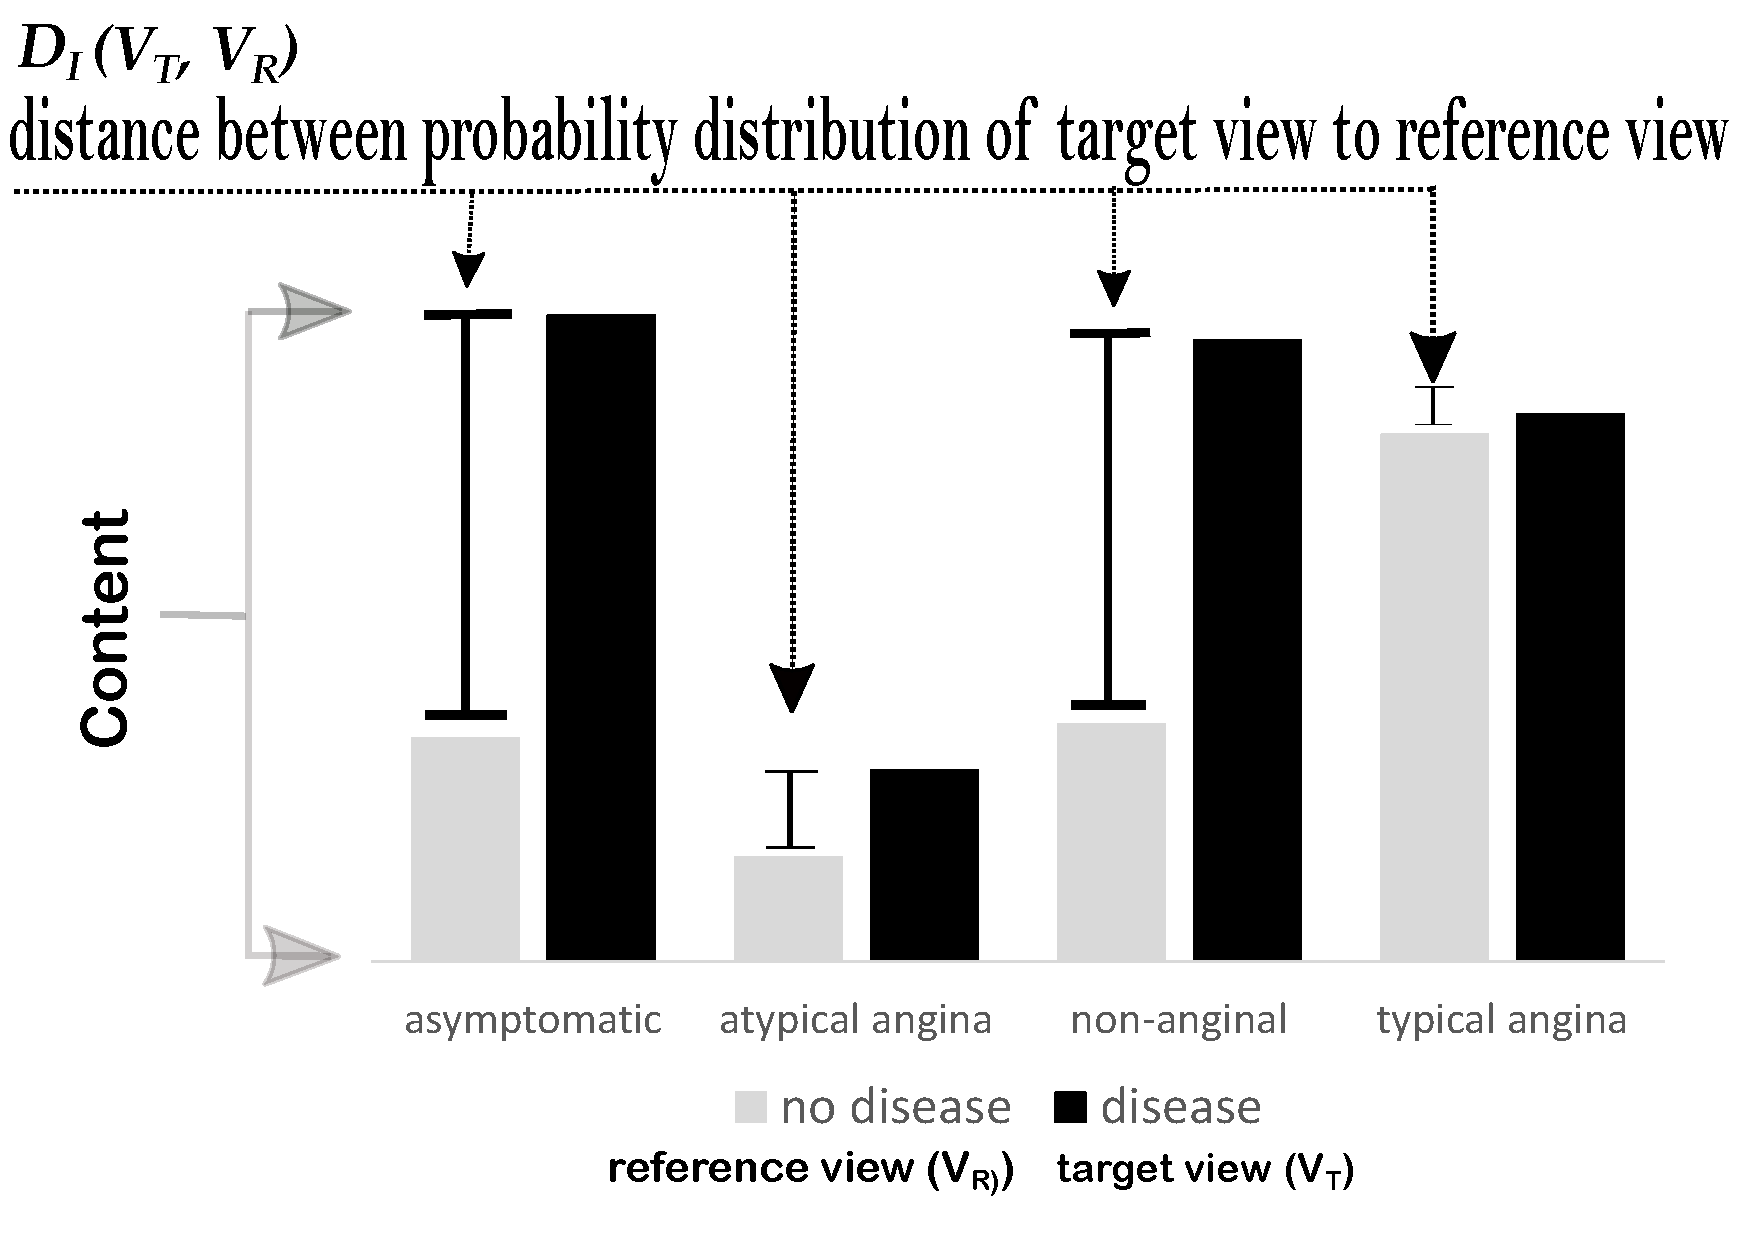
\includegraphics[width=2.5in]{figures/introduction/pre1}
		\caption{The content of view and the distance of $(V_T,V_R$)}
		\label{fig:pre1} 
	\end{subfigure}
	
	\begin{subfigure}[b]{0.40\textwidth}
		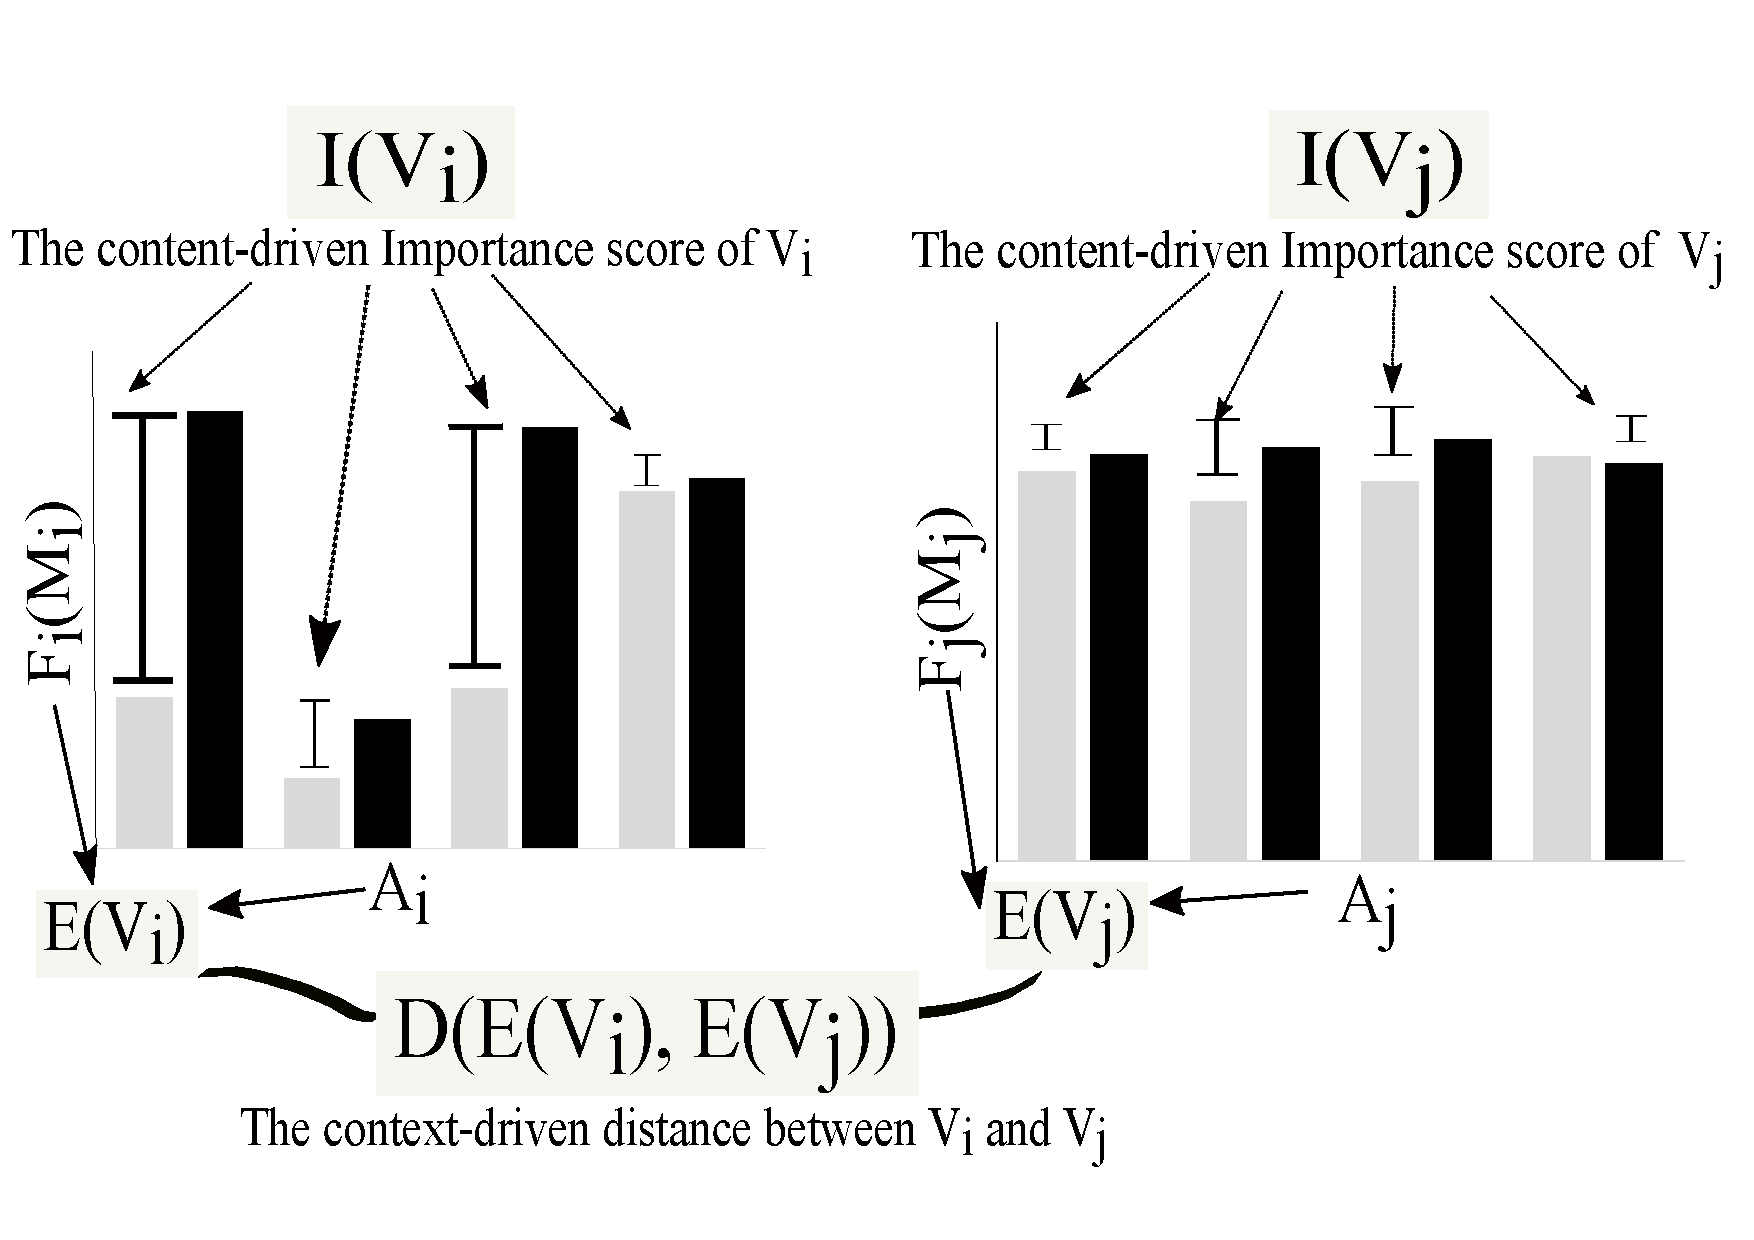
\includegraphics[width=2.5in]{figures/introduction/pre2}
		\caption{The context of views }
		\label{fig:pre2}
	\end{subfigure}
	\caption[content vs context]{Content vs. Context of views.}
	\label{fig:pre}
\end{figure}


The difference betweeen content and context is described in Figure \ref{fig:pre}. Content as in Figure \ref{fig:pre1} is the probability distribution of the aggregated query result whereas, Context as in Figure \ref{fig:pre2} is described as a set containing the name of the attribute, measure and function used to generate the view.  

\subsubsection{Content-Driven Deviation}
This approach measures how different a view is in relation to some reference subset of data. Hence, in order to compare the views, we need to have target subset and a reference subset of the $D_B$. The reference data set can either be another subset of $D_B$ or whole $D_B$. The example that we used are target subset $D_T$ is the subset of patients who has heart disease and the reference subset $D_R$ is the opposite, it consists of all patients without heart disease. For the content evaluation, we use a deviation-based approach as employed in \cite{Vartak2015}, \cite{Vartak2014}. The deviation value between target view and reference view is called as importance score. 

The importance score of $V_{T}$ is measured in terms of a score that captures the distance between probability distribution of target view $V_{T}$ over $D_T$ and probability distribution of reference view $V_{R}$  over $D_R$, it can be seen in Figure \ref{fig:pre1} and can be formally defined as follow:

\begin{equation}
D_I\left(V_T,V_R\right) = dist\left(\mathcal{P}\left[V_T\left(D_T\right)\right], \mathcal{P}\left[V_R\left(D_R\right)\right]\right)
\label{importance_score}
\end{equation}

where $ D_I\left(V_T,V_R\right) $ is the importance score of $ V_T$ and \textit{dist} is the Euclidian distance or other distance functions. To confirm that both views have the same scale, each view is normalized. The normalized probability distribution can be calculated by $ \frac{ Ag_1 }{G},\frac{ Ag_2 }{G},\frac{ Ag_3 }{G},\frac{ Ag_4}{G}.....,\frac{ Ag_n }{G} $ where $ \frac{Ag_i }{G}  $is the aggregated value of $ F $ over $ M $ for the group-by $ A $, and  $ G= $ $\sum_{p=1}^{n}{Ag_n}$. 

The higher distance between target view $ V_T $ and reference view $ V_R $, translates in to higher importance score $ D_I $. When judging the importance score of a view, it is believed that a view with large deviation from a reference view is more likely to reveal trends and patterns that are of high interest to the user \cite{Vartak2015}, \cite{Vartak2014}. 

\subsubsection{Context-Driven Deviation}
Content-driven deviation exposes the quality of individual view compared to reference view that can be other subsets of data or the whole data set. However, since the views are recommended as a collection or set which consists of multiple views, the quality of the whole set is as important as the quality of individual views\cite{Vartak2017}. The exiting approaches which only based on the content-driven only exposes the quality of individual view which are suffer from redundancy. To overcome this issue, we consider context-driven deviation that measures how different are the individual view within the set of views that recommended to the user. We believe that a diverse set of views is likely to be more informative than a monotonous set of views that have high importance score but provide little-added information relative to each other. 

To recommend a set of views which diverse among all views needs a diversity function. The notion of diversity has been widely used in recommendation systems for maximizing information gain and minimizing redundancy\cite{Zhang2008,Rafiei2010, Yu2009, Vieira2011}. There are various definitions of diversity, but most of them can be classified in one of this categories: (i) content-based diversity, means selecting results based on dissimilarity to each other \cite{Vieira2011,Khan2014}; (ii) novelty-based diversity selects the results that contain new information compared to the previous results which have been presented to the user\cite{Clarke2008}; (iii) semantic-based diversity selecting results that based on categories or topics\cite{Rafiei2010}. Depending on the type of recommendation system, different measures of diversity are used. 

For recommending a diverse set of visualizations, we deploy a diversity measure based on the context of the views. Intuitively, views generated using a different set of attributes, measures and functions are likely to provide different information. In order to determine the contextual distance between two views, we need to define a measure for calculating the distance between its context of two views. For instance, let $ V_i $ and $ V_j $ be two views that are generated using some aggregated queries over $D_Q$, and $ (ctx) $ means the context of the view. Also, let $ V_{i}(ctx) $= <$ A_i $,$ M_i $,$ F_i $> and $ V_{j}(ctx)=<A_j,M_j,F_j $> where { $ A_i , A_j \in \mathbb{A}, M_i, M_j \in \mathbb{M}, F_i, F_j \in \mathbb{F} $}. As comparing $ V_{i}(ctx)$ and $ V_{j}(ctx) $ require set comparison, we use Jaccard similarity measure which is a well-established similarity measure for sets of categorical data.  The Jaccard method measures similarity between finite sets as intersection of sets over union of sets. Hence, the Jaccard similarity between two views can be measured as:
\newline

\centerline{$ J$($V_{i}(ctx), V_{j}(ctx) $)$ = \dfrac{| V_{i}(ctx) \cap V_{j}(ctx) |}{| V_{i}(ctx) \cup V_{j}(ctx) |} $}
\bigskip

The contextual distance $ div $  between two views can be defined as: 
\newline
\begin{equation}
div\left(V_{i}(ctx), V_{j}(ctx)\right) = 1- J\left(V_{i}(ctx), V_{j}(ctx)\right) 
\label{diversity_score}                 
\end{equation}

% Diversity weight 

\bigskip
All symbols in this paper are explained in the Table of Symbols and it can be seen in Table \ref{tab:tab-symbols}.

\begin{table}
	\caption{Table of Symbols}
	\label{tab:tab-symbols}
	\begin{tabular}{ccl}
		\toprule
		Symbol &Description\\
		\midrule
		k & size of k\\
		S & selected set of views which equal to k\\
		S* & optimum set of views \\
		V & set of all possible generated views\\
		X & set of all remaining views which not included in S\\
		$ A $ & attribute / member of set of attributes $ \mathbb{A} $\\
		$ M  $& meassure  / member of set of meassures $ \mathbb{M} $\\
		$ F $ & agg. func. / member of set of agg. funcs. $ \mathbb{F} $\\
		$ Q $ & a general format for query \\
		$ T_T $ & a query predicate of the target subset\\
		$ T_R $ & a query predicate of the reference subset\\
		$ D_B  $& a multi-dimensional database \\
		$ D_Q  $& an example subset of $ D_B  $\\
		$ D_T  $& a target subset of $ D_B  $\\
		$ D_R  $& a reference subset of $ D_B  $\\\
		$ V_T  $& a target view\\
		$ V_R  $& a reference view \\
		$ V_i  $& an example of one view \\
		$ D_I$($S$)  & importance score of selected set of views\\
		$ div $  & the contextual distance between two views\\
		$ f$($S$,$div$) & diversity score of selected set of views\\
		$ F$($S$)  &  objective function value of the set S \\
		$ U$($V_i$) &  the utility score of each candidate view \\
		$ maxD_I$ &  the maximum value of importance\\
		\bottomrule
	\end{tabular}
\end{table}

\subsection{Problem Definition}
There are two main evaluation variables that used in this work, which are \textit{effectiveness} and \textit{efficiency}. The proposed recommendation visualization systems should recommend set of views with the high importance score as well as diverse among views. Moreover, it should has high efficiency in terms of costs due to all computations are running on the fly. 

\subsubsection{Effectiveness}
In this section, we formally define the problem of the quality of recommended views. \textit{i-DiVE} scheme designed to recommend a set of k views that are high importance as well as diverse among themselves. In particular, given a query subset $D_T$ as the target subset and a reference subset $D_R$ , set of all possible views V, our objective is to select a set  S* $\subseteq V $ where |S*| = k, such that the importance score of the views in S* and their mutual diversity is maximized. To achieve this goal, there are two components that need to be considered, the importance score of a set of views S, and the diversity score of the set S. 

\textit{The importance score computation}. The importance score of the set S is calculated as the normalized average value of the importance measure of each view in S, it can be defined as:
\newline

\centerline{$ D_I\left(S\right)= || \dfrac{1}{k} \sum_{i=1}^{k} D_I(V_i, V_R) ||, V_i  \in S $}
\bigskip

To normalize the importance score of set S to range 0 - 1, it can be by dividing the average of importance score of the set S with the maximum importance score. The maximum importance score of each views is not as straight forward, it depends on the real data. However, since the data generated by view is normalized (equation \ref{importance_score}), the range of the probability distribution representing each view is between 0 and 1. The maximum distance between two values in two different probability distributions can only be at most 1. Since, the sum of all values in a probability distribution can be 1, there can only be at most two pairs of values across two distributions with mutual distance of 1. This results in Euclidian distance of $ \sqrt{(1^2+1^2 )}= \sqrt{2} $. As a result, the maximum importance score to be equal to $\sqrt{2}$. 

\textit{The diversity score computation}. There are several diferent diversity functions have been employed in the literature \cite{Vieira2011,Khan2014},\cite{Clarke2008}, among which previous research has mostly focused on measuring diversity based on either the average or the minimum of the pairwise distances between elements of set \cite{Wu2014}. We focus on the first of those variants (i.e., average), as it considers all the views in S. Given a distance matric $ div\left(V_i, V_j\right) $ as given in equation 2, the diversity of a set S can be measured by a diversity function $ f\left(S,div\right) $ that captures the dissimilarity between the views in S, defined as:
\newline

$ f\left(S,div\right)= \dfrac{1}{k\left(k-1\right)}  \sum_{i=1}^{k} \sum_{j>i}^{k} div\left(V_i,V_j\right) ,V_i,V_j  \in S $
\newline

In order to capture both importance and diversity in the set of recommended views, we define a hybrid objective function that considers both importance and diversity when generating set S. Specifically, for a subset S $\subseteq V$ an objective function is formulated as the linear weighted combination of the diversity function $ f\left(S,div\right) $ and importance score, $ D_I\left(S\right) $ which is defined as:
\newline
\begin{equation}
F\left(S\right) =  \left(1-\lambda\right).D_I\left(S\right) + \lambda.f\left(S,div\right)
\label{objectif_function}
\end{equation}
\newline
where $ 0 \leq \lambda \geq 1 $ is employed to control the contribution between importance and diversity in the hybrid objective function. The higher values of $  \lambda $ result in a set of more diverse views whereas lower values of $ \lambda $ generate a set of the most important views that might be similar to each other. 
Given the hybrid objective function, our goal is to find an optimum set of views  $ S^* $ that maximizes the objective function $ F\left(S\right) $: 

\begin{equation}
S^* = \underset{\underset{|S|=k} {S \subseteq V}} {\mathrm{argmax}} F\left(S\right) 
\label{argmaxF}
\end{equation}



\subsubsection{Efficiency}
In the section before, we explained in terms of quality of the results which is presenting views based on importance and diversity. This section defines the issue in terms of efficiency, as explained in the preliminaries section that in case of the modest data which has small number of dimensions, it can generate large number of views. Meanwhile, views which want to be presented to users only in small number (top-k views) and all computation will be done on the fly. We need the scheme that robust in terms of the quality of results and also the running time (costs), in particular for the case of interactive visualization recommendation systems. 

It has been mentioned a lot in the literatures \cite{Vartak2014, Vartak2015, Ehsan2016} that the main issue of the visualization recommendation systems is the query execution. To deal with the query costs, there are several approaches that proposed, such as query results caching\cite{Khan2014}, shared computation among views, combine target and reference query, combination of multiple aggregates, combination of multiple group by, and parallel query and execution, \cite{Vartak2015},\cite{Wu2014}. 

However, in this work, we propose \textit{i-DiVE} scheme that equipped by pruning ability which able to reduce the number of query executions, the detail is presented in the proposed methods section. 











% ============================================== %
% PROPOSED METHODS %
% ============================================== %


\section{PROPOSED METHODS}

In this section, we present our \textit{i-DiVE} scheme for evaluating top-k visualizations that are of high importance to the user as well as diverse among themselves. Computing a set of top-k visualizations that maximize an objective function is a combinatorial optimization problem. Therefore, \textit{i-DiVE} employs Greedy algorithms which are popular for solving such optimization problems. Greedy algorithms have been shown to be efficient and provide good approximations to the optimal solutions \cite{Yu2009}, \cite{Vieira2011}, \cite{Smyth2001}. Generally, a Greedy algorithm starts with an empty set S and iteratively selects a view to be added to S that maximizes the objective function score $F\left(S\right)$. In most works, this approach is called Greedy Construction Algorithm. The key ingredient of any Greedy algorithm for solving an optimization problem is the Objective function itself that needs to be maximized. 

Before presenting the details of how \textit{i-DiVE} evaluates the hybrid objective function using greedy algorithm, we first present two baseline objective functions for evaluating top-k visualizations.

\subsection{Baseline Algorithms}

Current visualization recommendation systems consider only importance when ranking a view for recommendation \cite{Vartak2014, Vartak2015, Ehsan2016}. Thus, the objective function value of a set of k views S, is computed as the sum of the importance score of each view in S. This approach does not consider how the diversity score of S is effected when a new view is added to S. 
As discussed in the introduction, the recommendations generated solely on the basis of importance score, suffer from the redundancy problem.  The extreme solution to overcome the redundancy in the top-k set S is to select views such that the diversity score of S is maximized. This leads to two extreme baseline solutions, one based only on the importance score of the views and second based on only diversity score of the views. 

\begin{algorithm}
	\SetAlgoLined
	\KwIn{Set of views V and result set size k }
	\KwOut{Result set $ S \geq V $, |S| = k}  
	$S \leftarrow \left[v_i, v_j\right] $ get  two most distant views\;
	$X \leftarrow  \left[V \backslash S\right]$\;
	$i \leftarrow len\left(S\right) $\;
	\While{i < k}{
		\If{Pruning = True}{
		$ enablePruning $\;
		}
		\For{$j$ in set $X$}{
			$ max_v \leftarrow argmax F\left(X\left[j\right],S\right) $\;
		}
		$ S.add\left(max_v\right) $\;
		$ X.remove\left(max_v\right)$\;
		$ i  \leftarrow  i + 1 $\;
	}
	return S
	\caption{\textit{i-DiVE} Greedy}\label{i-DiVE-Greedy}
\end{algorithm}



\subsection{\textit{i-DiVE-Greedy} Scheme}

In order to capture both importance and diversity in the recommended top-k views, \textit{i-DiVE} employs a greedy construction algorithm to iteratively select views that maximize the hybrid objective function $F\left(S\right)$ as presented in equation 3, and it is called as \textit{i-DiVE-Greedy} scheme. The tradeoff between the importance score of a view and its distance from the already selected views in S, is controlled using the weight parameter $\lambda$. The smaller values of $\lambda$ can be selected by the user for a top-k set that contains views with high importance score. Whereas, the higher values of $\lambda$ can be selected for more diverse set of views. 
The details of the \textit{i-DiVE-Greedy} scheme are given in Algorithm \ref{i-DiVE-Greedy}. In particular, \textit{i-DiVE-Greedy} initializes the set S with two most distant views. The distance between all the views is calculated using the distance function as given in equation 2. In each iteration, a new view is selected from remaining views X and added to S. Thus, \textit{i-DiVE-Greedy} assigns a utility score to each candidate view which is based on the hybrid objective function $F\left(S\right)$ as defined in equation \ref{objectif_function}. The utility score of each candidate view $V_i$ in X is computed as: 

\begin{equation}
U\left(V_i\right)= \left(1-\lambda\right).D_I\left(V_i, V_R\right) + \lambda.setDist\left(V_i, S\right)
\label{utility_each_candidate}
\end{equation}

Where $ setDist\left(V_i, S\right) = \dfrac{1}{|S|} \sum_{\underset{V_j \in S}{j=1}}^{|S|} div\left(V_i, V_j\right) $
\newline

Thus, the view with highest utility score in each iteration is selected and added to S.

%\textit{i-DiVE-Greedy scheme costs.} There are four types of costs that required to run \textit{i-DiVE} scheme, as follows:
%
%\begin{itemize}
%	\item Query cost $C_Q$: Cost that needed for the query execution, the cost of $C_Q$ depends on the query itself and the number of rows (tuples) of the dataset. This cost depends on CPU and I/O cost but it dominated by I/O costs. 
%	\item Deviation/importance cost $ C_I $: The deviation computation cost is relatively cheap due to this cost only compute the probability distribution of each view and calculate the distance between two probability distribution of views (target view and reference view). The deviation equation can be seen in equation 1. This cost only from CPU costs.
%	\item Diversity cost $C_D$: Cost which required not only the computation of dissimilarity between two context views but also for whole diversity computation. This cost also only from CPU costs. $C_D$ depends on the number of views and the diversity algorithm that used, e.g. Greedy construction is cheaper than Swap, the cheapest is Random Algorithm. 
%	\item Visualization cost $C_V$: Cost which needed for plotting visualization and it only depends on CPU cost. 
%\end{itemize}

The time complexity of Greedy Construction algorithm has two components. One is the query execution cost for generating all views and computing the importance score $C_Q + C_I$. Second is the diversity cost $C_D$ that computing set distance of each view from the views already in S . The query execution cost is dominated by the I/O cost of retrieving the query results. Whereas, the set distance cost is the CPU cost of calculating the Jaccard similarity measure. The set distance cost is of $ O$($kn$) where k is the size of subset of views S and $ n $ is the number of all possible views. The query execution cost is of $ O$($n$) as the content of each view is generated only once. Although, greedy algorithm is very efficient as the number of attributes $\mathbb{A}$, measures $\mathbb{M}$ and aggregate functions $\mathbb{F}$, increase the number of views that need to be generated increase exponentially. Therefore, in order to reduce the cost of evaluating top-k views \textit{i-DiVE-Greedy} employs effective optimization strategy as elaborated next. 


\subsection{\textit{i-DiVE-Greedy} Optimization}

In order to recommend a small subset of views, the utility score of all possible views need to be computed. Since, the utility score of each view is based on its deviation from the reference view, the content of the view must be generated by executing the view query. However, only few views are eventually recommended to the user and rest of the views are discarded. Clearly, this approach would hinder the performance of the visualization recommendation systems for high dimensional datasets. Thus, motivated by the need to reduce the number of views that need to be generated, \textit{i-DiVE-Greedy} employs a pruning based optimization technique. 

The proposed optimization technique is based on the observation that the utility score of each view is a weighted sum of two different measures; 1) the importance score of view from the reference view and 2) diversity score of a view from S. The diversity score of a view requires only CPU computations and is thus a faster operation. Whereas, computing the importance score of a view by comparing the target view to the reference view incurs high I/O cost and CPU cost. The high I/O cost is dominated by the query executions. The CPU cost dominated from the computation of Euclidian distance between two probability distributions. 

Therefore, under that observation, \textit{i-DiVE-Greedy} leverages the diversity score of a view to decide whether a view query should be executed or not. Specifically, the views that will not make it to the recommended subset eventually, are identified early on the basis of their set distance score and are pruned. The view query is executed only for the remaining views to compute complete utility score for those views. For example, assume that a user wants to get some views from visualization recommendation systems and she uses $\lambda$ = 0.7. The $\lambda$ value equal to 0.7 means that the diversity score contribution to the utility score will be 70 percent and the contribution of the importance score will be 30 percent, as it can be seen in equation \ref{objectif_function}. Thus, on the basis of the diversity score only, low quality views can be pruned early. The details of the pruning method are given below.

We applied Max-Min pruning method as presented in \cite{Khan2015}. First, \textit{i-DiVE-Greedy} selects two most distant views as the initialization. In each iteration, instead of computing a complete utility score for each view, only partial utility score is computed. The partial utility score has two components; 1) the actual diversity score of the view from S and 2) the estimated importance score of view from the reference view. The partial utility score is defined as:

\begin{equation}
U'\left(V_i\right)= \left(1-\lambda\right).D_{I-est}\left(V_i, V_R\right) + \lambda.setDist\left(V_i, S\right)
\label{partial_utility}
\end{equation}
\newline
where  $ D_{I-est}\left(V_i,V_R\right) $ is the estimated importance score of $ V_i $ from $ V_R $. Without generating the view query, it is only possible to estimate the minimum and maximum deviation of a view from reference view. The minimum distance between two probability distributions can be 0 so we estimate minimum importance score as 0. The maximum importance score as explained in the preliminaries section is equal to $ \sqrt{2} $. Let us denote the minimum possible importance score of a view by $ minD_I\left(V_T,V_R\right) $ and maximum importance score by $ maxD_I\left(V_T,V_R\right) $.

Using the $ minD_I\left(V_i,V_R\right) $ and $maxD_I\left(V_i,V_R\right) $ values in the equation \ref{partial_utility}, we can calculate minimum utility score $ minU'\left(V_i\right) $ and maximum utility score $ maxU'\left(V_i\right) $  for all candidate views. The views that have $ maxU'\left(V_i\right) $  score less than the $ minU'\left(V_i\right) $score of any other view are pruned. This Max-Min pruning approach called as \textit{i-DiVE-Greedy-Static-Pruning}. This approach generates same set of recommended views as generated by the \textit{i-DiVE-Greedy} without pruning. This is due to the fact that in each iteration \textit{i-DiVE-Greedy } selects the view with highest utility score to be added to S. If the maximum possible utility score of a view is less than the minimum possible utility value of another view in the candidate list, it cannot be the winner with the highest utility score.

This Max-Min pruning approach has been mentioned in \cite{Khan2015} and it has good performance in pruning. However, in that literature, the points has very diverse values. To the contrary, in this work, the context of view only has three dimentions. Hence, by using three dimentions and computing the diversity score to small set of view S, the partial utility value may not diverse as in the literature. We were in doubt if this pruning scheme was able to prune significanly in this work. 

% it will be a good idea to discuss the characteristic of jaccard similiarity measure here. When comparing two sets with three items in each, there can only be three possible distance values, 1/3, 2/3 and 3/3. So pruning only on the basis of contextual distance may not be feasible for smaller lamda values. Then you can discuss why this problem is expected to not happen in the swap algorithm. %
\begin{algorithm}
	\SetAlgoLined
	\KwIn{Set of views V and result set size k }
	\KwOut{Result set $ S \geq V $, |S| = k}  
	$S \leftarrow $ Result set of only importance or only diversity\;
	$X \leftarrow  \left[V \backslash S\right]$\;
	$F_{current} \leftarrow 0 $\;
	$  improve \leftarrow  True $\;
	\While{improve = True}{
		%		\If{Pruning = True}{
		%			$ enablePruning $\;
		%		}
		\For{$i$ in set $X$}{
			$ S' \leftarrow S $\;
			\For{$j$ in set $S$}{
				\If{ $ F\left(S'\right) < F\left(S \backslash S[j] \cup X[i]\right) $}{
					$ S'  \leftarrow S \backslash j \cup X[i] $  \;
				}
			}
			\If{ $ F\left(S'\right) > F\left(S\right) $}{
				$ S  \leftarrow S'$
			}
		}
		\eIf{ $ F\left(S\right) > F_{current} $}{
			$ F_{current}   \leftarrow F\left(S\right) $\;
			$  improve \leftarrow  True $\;
		}{
		$  improve \leftarrow  False $\;
	}
}
return S
\caption{\textit{i-DiVE} Swap}\label{i-DiVE-Swap}
\end{algorithm}

\subsection{\textit{i-DiVE} Scheme using Swap technique}

Beside of using Greedy technique, we also proposed another approach which is using swap technique. Swap is local search type algorithm, this algorithm starts with a complete initial set S, and try to achieve better result by interchanging the remaining views in X to the current set S. If the views in remaining X able to give better objective function value $ F $($ S $), then this view will be joined to the current set and one view in the current set that has the lowest contribution to the $ F $($ S $) will be removed. 

In this work, we proposed two types of Swaps which are \textit{i-DiVE-SwapI} which is Swap algorithm that initialized by the results of Only Importance and \textit{i-DiVE-SwapD} which is Swap that initialized by results of Only Diversity. Both of those Swap algorithms already have a good initialization, \textit{i-DiVE-SwapI} with all current views in set S which has the maximum of importance score and \textit{i-DiVE-SwapD} with the current set S which has the maximum of diversity score. The details of \textit{i-DiVE-Swap} algorithm can be seen in Algorithm \ref{i-DiVE-Swap}.

The complexity of Swap algorithm is dependent on the query execution time, the importance score computation $ D_I\left(V_i,V_R\right) $ for all views, the diversity score and computation of objective function F(S) in each iteration. The importance score $ D_I\left(V_i,V_R\right) $ is calculated only once and is independent of the number of iterations of Swap. However, the objective function evaluation time is of $ O\left(k^2 \right) $ and the number of times objective function value is computed depends on the number of iterations of the swap and the number of views $ n $ in the candidate list. In the worst case, swap algorithm can perform $ O\left(k^n \right)  $iterations.



To minimize the I/O cost of executing view queries, we again apply pruning method in Swap algorithm. \textit{i-DiVE-SwapI} uses the results of Only importance as the first initialization. Hence, in case of reducing query executions by pruning scheme, this algorithm cannot escape from executing all queries due to this algorithm uses result set of Only importance in the initialization that required to execute all queries in advanced. However, the second proposed swap algorithm which is \textit{ i-DiVE-SwapD}, this algorithm uses the result of Only Diversity as the set of initialization. This algorithm does not need importance score for the initialization, it means there is no query execution for the initialization and pruning scheme can be applied on it. The detail of \textit{ i-DiVE-SwapD} optimization using pruning scheme is explained below. 

\begin{algorithm}
	%	\SetAlgoLined
	%	\KwIn{Set of views V and result set size k }
	%	\KwOut{Result set $ S \geq V $, |S| = k}  
	%	$S \leftarrow $ Result set of only importance or only diversity\;
	%	$X \leftarrow  \left[V \backslash S\right]$\;
	%	$F_{current} \leftarrow 0 $\;
	%	$  improve \leftarrow  True $\;
	$ max_b  \leftarrow\sqrt{2} $\;
	%$ X' \leftarrow [] $\;
	\For{$i$ in set $X$}{
		\For{$j$ in set $S$}{
			$ d  \leftarrow setDist\left(X[i],S \backslash S[j]\right) $\;
			$ 	newX \leftarrow [S[j], X[i], d]$\;
			$ 	X'.append(newX)$\;
		}
	}
	$ 	X' \leftarrow sorted\_by\_d(X') $\;
	$ S' \leftarrow S $\;
	\eIf{ $ max_b == \sqrt{2} $}{
		\For{$i$ in set $X'$}{
			
			\If{ $ F\left(S'\right) < F\left(S \backslash X'[i][0] \cup X'[i][1], max_b\right) $}{
				$ 	X''.append(X'[i][1])$\;
			}
		}
		
		$n \leftarrow pi - len(S)$\;
		$samples \leftarrow X''[0\colon n]$\;
		$maxI\_S \leftarrow get\_maxI(S)$\;
		$maxI\_samples \leftarrow get\_maxI(samples)$\;
		
		\If{ $ maxI\_S > maxI $}{
			$ maxI \leftarrow maxI\_S$
		}
		\If{ $ maxI\_samples> maxI $}{
			$ maxI \leftarrow maxI\_samples$
		}
		$max\_b \leftarrow maxI$	
		
		\For{$i$ in set $X''$}{
			\For{$j$ in set $S$}{
				\If{ $ F\left(S'\right) < F\left(S \backslash S[j] \cup X''[i], max_b\right)  $}{
					$ 	X'''.append(X''[i])$\;
					$ I \leftarrow get\_I\_score(X''[i]) $\;
					\If{ $ F\left(S'\right) < F\left(S \backslash S[j] \cup X''[i], I\right) $}{
						$ S'  \leftarrow S \backslash j \cup X''[i] $  \;
					}
					\If{ $ I > max_b $}{
						$ max_b \leftarrow I $
					}
				}
			}
		}
		
	}{ 
	\For{$i$ in set $X'$}{$ .... $
		%			\If{ $ F\left(S'\right) < F\left(S \backslash X'[i][0] \cup X'[i][1]\right) $}{
		%				$ 	X''.append(X'[i][1])$\;
		%			}
		%			$ I \leftarrow get\_I\_(X''[i]) $\;
		%			\If{ $ F\left(S'\right) < F\left(S \backslash S[j] \cup X''[i], max\_bound\right) $}{
		%				$ S'  \leftarrow S \backslash j \cup X''[i] $  \;
		%			}
		%			\If{ $ I > max\_bound $}{
		%				$ max\_bound \leftarrow I $
		%			}
		
	}
	
}

\If{ $ F\left(S'\right) > F\left(S\right) $}{
	$ S  \leftarrow S'$
}
return S
\caption{\textit{i-DiVE} SwapD Pruning}\label{i-DiVE-SwapD-Pruning}
\end{algorithm}

\subsection{\textit{i-DiVE-SwapD} Optimization}

In order to apply pruning scheme in \textit{i-DiVE-SwapD}, as in the Greedy technique, we utilize the maximum importance score $maxD_I$. To run \textit{i-DiVE-SwapD}, for the first time, $maxD_I$ will be initialized by $\sqrt{2}$. All views in X will be tried one by one to the current set S. In each iteration, instead of computing a complete utility score for each view, only partial utility score is computed, as in equation \ref{partial_utility}. The partial utility score using actual value of diversity score and estimated value of importance score $maxD_I$ which is equal to $\sqrt{2}$.

If the view in X, by using importance score $maxD_I$ which is equal to $\sqrt{2}$ cannot perform better in terms of improving the objective function value to the current set S, those views will be pruned. This method is valid due to if the importance score set to the maximum and that view cannot improve the objective function of the current set, then there is no reason to know the actual value of importance by executing the query of that view. The pruning scheme which applied in \textit{i-DiVE-SwapD} is called \textit{i-DiVE-SwapD-Static-Pruning}.


% Compare with Greedy in terms of pruning performance%

\subsection{Adaptive Pruning Scheme}

All proposed pruning schemes including \textit{i-DiVE-Greedy-Static-Pruning} and \textit{i-DiVE-SwapD-Static-Pruning} are using static value of $maxD_I$ which is equal to $\sqrt{2}$. The main issue of using static value of $maxD_I$ is if the estimated value of maximum importance score $maxD_I$ too far from the real value of the importance score in the dataset, the pruning scheme may not working optimal. 

In order to get better performance of pruning scheme, instead of using static $maxD_I = \sqrt{2} $, we proposed Adaptive Pruning scheme, that can adapt the value of $maxD_I$ to the real values in the dataset. In order to estimate the $maxD_I$ which can close to the real value in the dataset, we use sampling method. 

We applied this adaptive pruning scheme to \textit{i-DiVE-Greedy} algorithm which called \textit{i-DiVE-Greedy-Adaptive-Pruning} and to \textit{i-DiVE-SwapD} algorithm as called \textit{i-DiVE-SwapD-Adaptive-Pruning} . 

%For instance, in the \textit{i-DiVE-SwapD-Adaptive-Pruning}, $maxD_I$ is initialized by $ \sqrt{2} $. If the view by using $maxD_I$ can improve the objective function value in the current set S, the real Importance score of this view will be computed which is by executing the query of its view. For instance, after executing its query, the real Importance value is 0.25, by using $ \alpha= 0.8 $, the $ EWMA_t  $ will be $ (0.8 *0.25) + ((1- 0.4)*\sqrt{2}) = 0.48 $, and the current $maxD_I$ will be set to 0.48, and it will be updated continuously. This EWMA method able to set the value of $maxD_I$ as close as the real values in the dataset, it should make pruning scheme works better. 











% ============================================== %
% EXPERIMENTAL EVALUATION %
% ============================================== %


\section{EXPERIMENTAL EVALUATION}

\begin{table}
	\caption{Parameters testbed in the experiments}
	\label{tab:tab-parameter}
	\begin{tabular}{ccl}
		\toprule
		Parameter &Range (\textbf{default})\\
		\midrule\
		datasets & Flights, \textbf{Heart disease}, Superstore\\
		sample queries & \textbf{10} \\
		diversity weight ratio & \textbf{3($ A $) : 2($ M $) : 1($ F $)} \\
		tradeoff weight $ \lambda $ & 0, 0.2, 0.4, \textbf{0.5}, 0.6, 0.8, 1 \\
		result set (size of \textit{k}) & \textbf{5}, 15, 25, 35\\
		prediction interval (PI) \% & 80 , 85, 90, 95, \textbf{97}, 98\\
		\bottomrule
	\end{tabular}
\end{table}

\begin{table*}
	\centering
	\caption{The list of Schemes (Algorithms)}
	\label{tab:tab-list-schemes}
	\begin{tabular}{ccl}
		\toprule
		Scheme &Description\\
		\midrule\
		
		Only Importance & Consider only importance \\
		Only Diversity   & Consider only diversity\\
		i-DiVE-Greedy & Consider both importance and diversity (Hybrid) using Greedy technique\\
		i-DiVE-SwapI & Hybrid using Swap technique and the initialization set generated by Only Importance \\
		i-DiVE-SwapD & Hybrid using Swap technique and the initialization set generated by Only Diversity \\
		i-DiVE-Greedy-Static-Pruning & i-DiVE-Greedy equipped with pruning scheme which use static max bound = $ \sqrt{2} $\\
		i-DiVE-Greedy-Adaptive-Pruning & i-DiVE-Greedy equipped with pruning scheme that uses adaptive max bound\\
		i-DiVE-SwapD-Static-Pruning &i-DiVE-SwapD equipped with pruning scheme that uses static max bound = $ \sqrt{2} $ \\
		i-DiVE-SwapD-Adaptive-Pruning & i-DiVE-SwapD equipped with pruning scheme that uses adaptive max bound\\
		\bottomrule
	\end{tabular}
\end{table*}

% Experiment Setup and Dataset % 

\textbf{\textit{Experiment Setup}}. This experiment running on Windows 10 64 bit, Intel Core i7-7700 CPU @ 3.60 GHz, RAM 16 GB. The experiment is developed using Python and run on Python version 3.6.3 with PostgreSQL as the database engine. In this experiments, we use three real datasets, as follows: 

\begin{itemize}
	\item Airline Dataset \footnote{http://stat-computing.org/dataexpo/2009/the-data.html}, it has 7 attributes, 4 measure attributes. The detail as follows: $ \mathbb{A}  $= year, month, week, day, carrier, origin, destination; $ \mathbb{M}  $= arrivaldelay, departurdelay, weatherdelay, distance. This dataset has 855,632 number of rows. 
	\item Heart Disease Dataset \footnote{http://archive.ics.uci.edu/ml/datasets/heart+Disease}, it has 14 attributes in total which are 9 attributes $ \mathbb{A} $ and 5 measure attributes $ \mathbb{M} $, $ \mathbb{A}  $= sex, cp, fbs, restecg, exang, slope, ca, thal, num; $ \mathbb{M} $ = age, trestbps, chol, thalach, oldpeak. This dataset has small number of rows (299 rows).
	\item Tableau Superstore Dataset \footnote{https://community.tableau.com/docs/DOC-1236}, it has 13 attributes, 4 measure attributes. The detail as follows: $ \mathbb{A} $= order\_date, ship\_date, ship\_mode, customer\_name, segment, country, state, region, city, postal\_code, category, subcategory, product\_name; $ \mathbb{M} $ = sales, quantity, discount, profit. There are 10,971 rows of this dataset.
\end{itemize}

% i-DIVE schemes compared to BF and Random % 

%\textbf{\textit{i-DiVE schemes performance compared to Brute Force and Random}}. Before we start to analyze the effectiveness and the efficiency of our proposed schemes, to check its performance, we run all schemes and compared to all baselines including Brute Force and Random selection. We run all schemes only using k=5 due to BF algorithm has running time limitation, BF complexity is $O$($n^k k^2$). Hence, it is not good idea to increase the number of k due to BF algorithm tests every possibility of the result set, it should has the highest overall objective function value $F\left(S\right)$ among all proposed schemes. Moreover, all algorithms also should have better performance than the Random algorithm. The results show that two extreme baselines (Only Importance and Only Diversity) are not able to acheive the optimal overall objective function value $F\left(S\right)$. Only importance that only considers importance score, the value of $D_I$($S$) almost same as BF algorithm but $f$($S,div$) worse than Random. To the contrary, Only Diversity that only consider diversity value, it has high $f$($S,div$) which very closes to the BF algorithm but $D_I$($S$) close to Random. 
%Other than that, our proposed schemes either based on Greedy technique or Swap have overall objective function value $F\left(S\right)$ close to BF and better than those two extreme baselines. 



%\begin{figure*}[t]
%	\centering
%	\subcaptionbox{Flight dataset}[.3\linewidth][c]{%
%		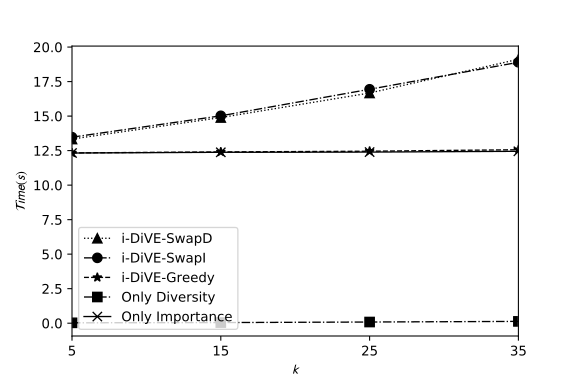
\includegraphics[width=.33\linewidth]{figures/results/output_time_flights}}\quad
%	\subcaptionbox{Heart disease dataset}[.3\linewidth][c]{%
%		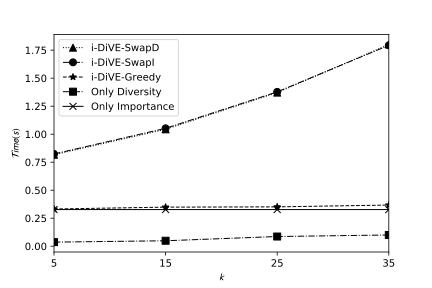
\includegraphics[width=.33\linewidth]{figures/results/output_time_heart}}\quad
%	\subcaptionbox{Superstore dataset}[.3\linewidth][c]{%
%		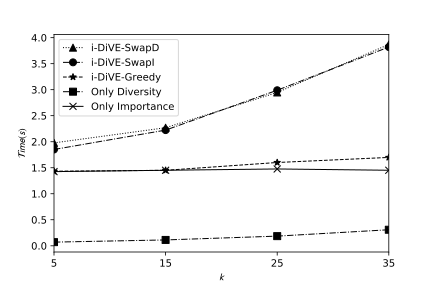
\includegraphics[width=.33\linewidth]{figures/results/output_time_superstore}}
%	\caption{Overall Costs/execution time while running on real datasets}	
%\end{figure*}

\begin{figure*}[t]
	\centering
	\subcaptionbox{Flights dataset}[.3\linewidth][c]{%
		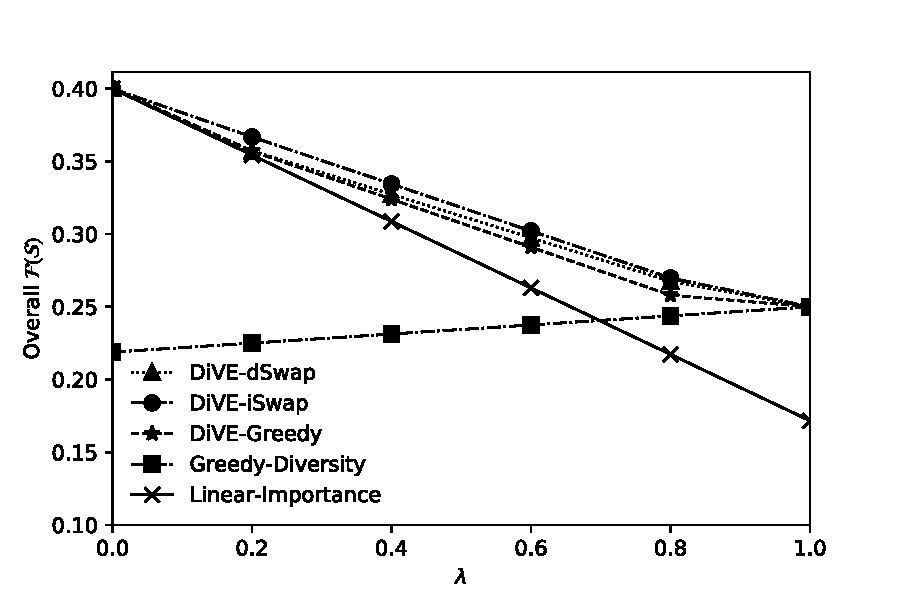
\includegraphics[width=.33\linewidth]{figures/results/tradeoff_flights}}\quad
	\subcaptionbox{Heart disease dataset}[.3\linewidth][c]{%
		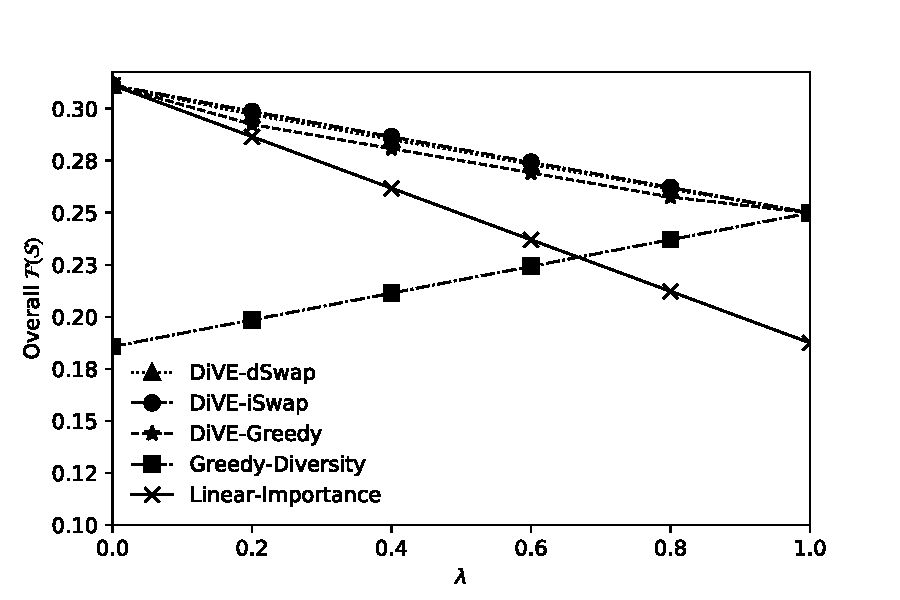
\includegraphics[width=.33\linewidth]{figures/results/tradeoff_heart_2}}\quad
	\subcaptionbox{Superstore dataset}[.3\linewidth][c]{%
		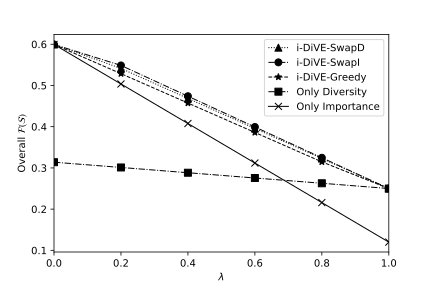
\includegraphics[width=.33\linewidth]{figures/results/tradeoff_superstore}}
	\caption{Impact of $\lambda$ to overall objective function value $F\left(S\right)$ while k = 5 and running on three real datasets}
	\label{fig:tradeoff_3_datasets}	
\end{figure*}

\begin{figure*}[t]
	\centering
	\subcaptionbox{Flights datasets}[.3\linewidth][c]{%
		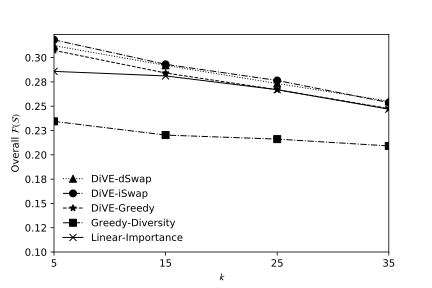
\includegraphics[width=.33\linewidth]{figures/results/objf_flights}}\quad
	\subcaptionbox{Heart disease dataset}[.3\linewidth][c]{%
		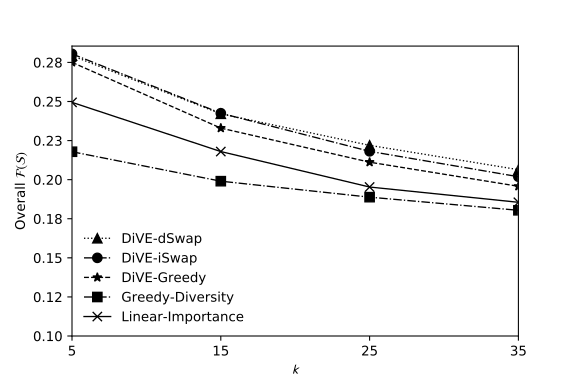
\includegraphics[width=.33\linewidth]{figures/results/objf_heart_2}}\quad
	\subcaptionbox{Superstore dataset}[.3\linewidth][c]{%
		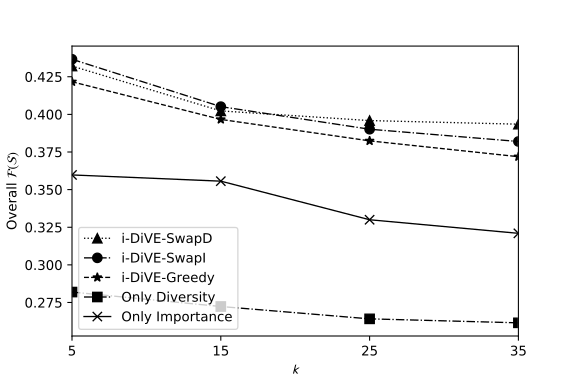
\includegraphics[width=.33\linewidth]{figures/results/objf_superstore}}
	\caption{Overall objective function value $F\left(S\right)$ using different value of k and running on three real datasets}
	\label{fig:objf_3_datasets}
\end{figure*}


\subsection{Effectiveness Evaluation}
%  Prolog of the quality of the results evaluation%
To test the performance of our proposed approach, we run the experiments using three real datasets which are flights dataset, heart disease dataset, and superstore dataset. In order to present the representative result, for each dataset, we execute ten random queries as shown in Table \ref{tab:tab-parameter}. Afterwards, we calculate the average of all results as the final result. We examine the performance of our proposed schemes in term of the quality of the result (effectiveness) and the efficiency. The detail results of the experiments which using different value of parameters as summarized in Table \ref{tab:tab-parameter} is elaborated next. 
 
 % The Impact of \lambda to the overall objective function value %
 
\textbf{\textit{The impact of parameter weight $\lambda$ to the overall $F\left(S\right)$}}. One of the advantage \textit{i-DiVE} scheme is users can decide what kind of the results that they want by changing the value of weight $\lambda$. The main function of $\lambda$ is this weight can be used to tradeoff between importance and diversity, it is explained in equation \ref{objectif_function}. Figure \ref{fig:tradeoff_3_datasets} shows the impact of $\lambda$ to the overall objective values $F\left(S\right)$ by fixed k equal to 5, where $ 0 \leq \lambda \geq 1 $. We can see in this figure that in the beginning when the $\lambda$ is close to 0, means the role is dominated by the importance score, Only importance has high overall objective function value $F\left(S\right)$ but it will decline gradually while increasing of $\lambda$. To the contrary, the Only Diversity is the opposite, it has the high overall objective function value when the $\lambda$ equal to 1, which means the diversity gets the full role. Hence, there is a crossover between Only importance and Only Diversity, this crossover shows the role balancing between importance score and diversity score. Futhermore, our proposed schemes have stable performance in all various $\lambda$ value and its  $F\left(S\right)$ value always better than Only importance and Only diversity. 

\begin{figure}
	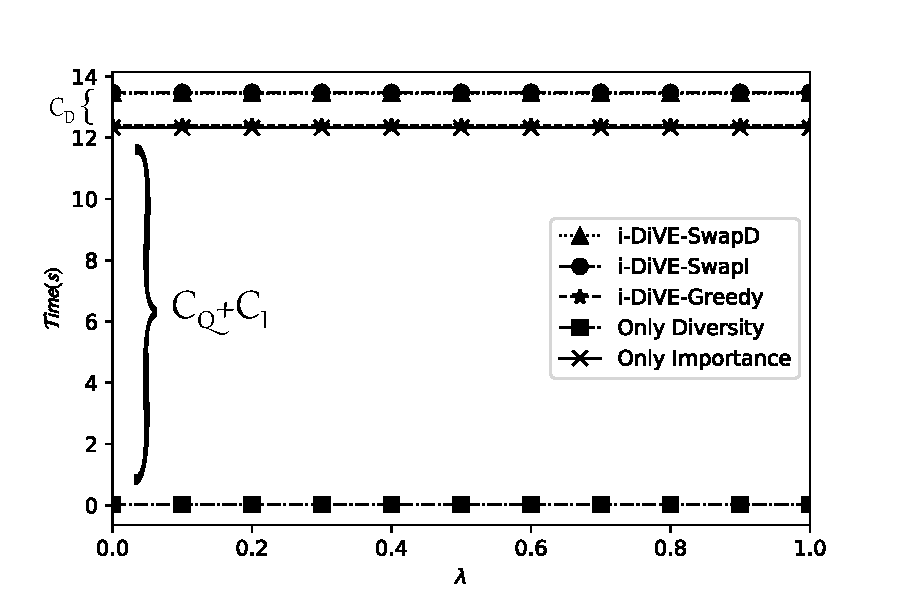
\includegraphics[width=3in]{figures/results/output_time_flights_lambda}
	\caption{Total time in seconds to execute schemes on flights dataset using k =5. It shows that costs are dominated by query costs}
	\label{fig:cost_flights}
\end{figure}

In addition, as shown in Figure \ref{fig:tradeoff_3_datasets}, there is unbalance between importance score of the set $D_I$($S$) and diversity score of set $f$($S,div $). It can be seen by the shape of the graphs while increasing the value of $\lambda$. When $\lambda$ value is small, the overall objective function value in the highest position and it decrease gradually while $\lambda$ is increased.  It happens due to unbalance of the real value of importance score and diversity score. The range value of diversity score can be predicted. As mentioned in the preliminaries section, this work uses three combination of context of the view which is $A, M, F$ (attributes, measures, and aggregate functions). According to the equation \ref{diversity_score}, the range value of diversity score is between 0 and 1. Let assume that the number of k equal to 3, to calculate the dissimilarity among three views that each view has three dimensions, the diversity value of the set which contains of three views $f$($S,div $) will be less than 0.5. As we know that the diversity value of set $f$($S,div $) decrease while k is increasing. On the other hand, the importance score cannot be predicted, the real value of importance depends on the real value inside the dataset. We only know that the maximum of importance score is $\sqrt{2}$. Due to this reason, it is not surpising if the shape of the graphs are not balance. The real importance score of the set $D_I$($S$) can be seen while the $\lambda$ = 0, in this moment, there is no contribution for diversity. Otherwise, the real diversity score of the set $f$($S,div $) can be seen while the $\lambda$ = 1.0. 




 % The Impact of k to the overall objective function value %
 
\textbf{\textit{The impact of k to the overall objective function value $F\left(S\right)$}}. It has been explained the impact of $\lambda$ to the overall objective function value $F\left(S\right)$. In this section, we explain the overall objective function value $F\left(S\right)$ by increasing k. Figure \ref{fig:objf_3_datasets} shows the overall objective values $F\left(S\right)$ by using different number of k. As shown in those figures, the value of $F\left(S\right)$ decrease while increasing the value of k. There are two reasons why this moment happens. First, to get the importance score from the set $D_I$($S$), sum of all importance score of views will be divided by the number of views or the number of k, increasing the number of k means increasing the divisor. Second, the diversity score of a set of views $f$($S,div $) also depends on the number of k. While k is increasing, the diversity score of the set will decrease, due to the score of $f$($S,div $) is yielded from the sum of all distance of views divided by $ k*(k-1)$. Hence, the more views selected, the probability to get similar views will be high and the score of diversity will be declined. 

The most important point in this results is our proposed schemes always have better overall objective function value $F\left(S\right)$ compared to the two extreme baselines in various number of k. Overall, the rank of the scheme performance in terms of the overall objective function value $F\left(S\right)$, start from the highest are \textit{i-DiVE-SwapI}, \textit{i-DiVE-SwapD}, and \textit{i-DiVE-Greedy} respectively.   



\subsection{Efficiency and Pruning Scheme Evaluation}

% Efficiency and Pruning Scheme%

\begin{figure}
	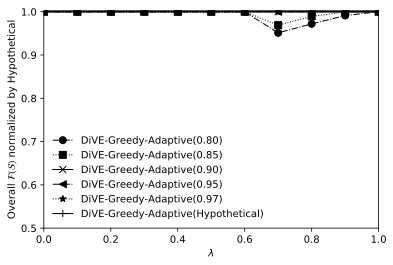
\includegraphics[width=2.9in]{figures/results/impact_lambda_to_PI_sampling_greedy_pruning}
	\caption{Impact of $ \lambda  $ to the performance of \textit{i-DiVE-Greedy-Adaptive-Pruning} with different of PI in terms of the effectiveness, running on Heart disease dataset using k = 5. Using PI 80 and PI 85 can reduce the quality of the result while the $\lambda$ value is low}
	\label{fig:impact_lambda_to_PI_sampling_greedy_pruning}
\end{figure}
\begin{figure}
	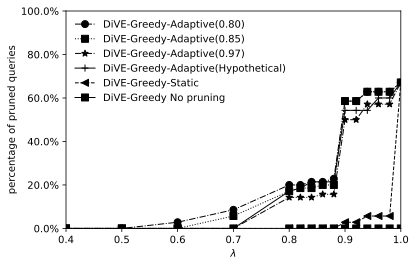
\includegraphics[width=2.9in]{figures/results/pruning_performance_greedy}
	\caption{Impact of $\lambda$ to the pruned queries of \textit{i-DiVE-Greedy} scheme, running on Heart disease dataset using k = 5. Using PI-97 able to prune queries around 20 percent while $\lambda$ higher than 0.8}
	\label{fig:pruning_performance_greedy}
\end{figure}


% Overall execution time / Overall costs to run all schemes%

\textbf{\textit{The total of execution time to run proposed schemes}}. In order to start analyzing the efficiency, we need to know the main issue in term of costs. Figure \ref{fig:cost_flights} shows the example of exactly time that needed to run schemes on flights dataset. It shows Only Diversity which only considering diversity and no query executions, it has very cheap in total costs. The costs of Only diversity almost same as Random even it closes to 0. Meanwhile, Only importance and \textit{i-DiVE-Greedy} seems in the same line but that was not exactly same. The total of diversity computations $ C_D $ of \textit{i-DiVE-Greedy} is very low, the total costs of \textit{i-DiVE-Greedy} is dominated by query costs $ C_Q $. Due to of this reason, the total execution time of \textit{i-DiVE-Greedy} closes to Only importance. Those are the proof that the total costs of all schemes execpt Only diversity are dominated by query cost $ C_Q $. 

The highest cost is the query cost $ C_Q $ in all datasets. However, heart disease dataset is the exception due to this dataset only has 299 rows, it is a very small dataset, due to this reason, the diversity cost $ C_D $ of Swap algorithms on k equal to 5 is higher than the query cost $ C_Q $, it only happens when the dataset is very small. 

\begin{figure}
	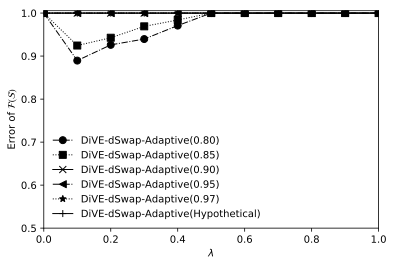
\includegraphics[width=2.9in]{figures/results/impact_lambda_to_PI_sampling_swapd_pruning}
	\caption{Impact of $ \lambda  $ to the performance of \textit{i-DiVE-SwapD-Adaptive-Pruning} with different of PI in terms of the effectiveness, running on Heart disease dataset using k = 5. Using PI 80 and PI 85 can reduce the quality of the result while the $\lambda$ value is low}
	\label{fig:impact_lambda_to_PI_sampling_swapd_pruning}
\end{figure}
\begin{figure}
	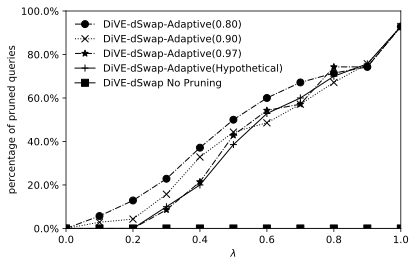
\includegraphics[width=2.9in]{figures/results/pruning_performance_swapd}
	\caption{Impact of $\lambda$ to the pruned queries of \textit{i-DiVE-SwapD} scheme, running on Heart disease dataset using k = 5. Adaptive pruning schame able to prune queries start from $\lambda$ 0.1, it has more pruned queries while $\lambda$ increased}
	\label{fig:pruning_performance_swapd}
\end{figure}


Due to the page limitation, all our experiments in three real dataset cannot be showed. Hence, for the next sections, we use heart disease dataset as our focus observation. 
% Static Pruning Scheme Performance%

%\subsubsection{Static-Pruning scheme performance}


% Impact of lambda (parameter to tradeoff between importance and diversity) to the pruned queries, running on Heart disease dataset %

\textbf{\textit{Impact of $\lambda$ to the pruned queries of \textit{i-DiVE-Greedy} scheme}}. In this work, we proposed two kind of pruning schemes, that are using estimated static value of maximum value of the importance score $maxD_I$ and using adaptive maximum value of importance score. 

The first our pruning scheme is using static value $maxD_I$. To check the performance of our pruning scheme, we run it to all real datasets using different value of $ \lambda $. We analyze the result by comparing the result of schemes with pruning enable on it and the schemes without pruning enable on it. The example result which running on heart disease dataset is shown in Figure \ref{fig:pruning_performance_greedy} . The static pruning scheme only able to prune queries while the value of $\lambda$ is high, closes to 0.9. As we expected, it is because the value of $maxD_I$ that too far from the real value of importance score. 

%\subsubsection{Adaptive-Pruning scheme performance}
To overcome the flaw in static pruning scheme, we also proposed adaptive pruning scheme which used dynamic value of the maximum importance score $maxD_I$. In order to get $maxD_I$ as close as possible to the real value of importance in the dataset, we applied sampling method. By using adaptive pruning, users also able to change the confidence and the margine error to tradeoff between time and precision. 

% Impact of lambda to the pruned queries for adaptive pruning scheme %

\textbf{\textit{Impact of $\lambda$ to the pruned queries of \textit{i-DiVE-SwapD} scheme}}. If static pruning scheme only able to prune queries while $\lambda$ closes to 0.9 and higher, in this section, we shows the adaptive pruning performance. Figure \ref{fig:pruning_performance_swapd} shows the performance of adaptive pruning scheme by using different value of $\lambda$. It shows the impact of $\lambda$ to the percentage of pruned queries. The adaptive pruning schemes especially \textit{i-DiVE-SwapD-Adaptive-Pruning} is able to prune queries significantly, pruning start while $\lambda$ closes to 0.2 and by increasing the $\lambda$, more queries can be pruned.


% The impact of query load to the pruning performance %

\textbf{\textit{The impact of query load to the pruning performance}}. As shown in Figure \ref{fig:objf_3_datasets}, that the actual value of importance score affects to the overall value of objective function $F\left(S\right)$ and the shape of the graphs. The next question is do the actual value of importance score also affects the pruning performance while using adaptive pruning scheme? We did experiments using heart disease dataset to answer this question. We lists all subsets in the heart disease dataset and classify those subsets to three categories: low, middle, and high. Low category consist of subsets that have mostly low value of importance score, high category is the opposite, and the middle category is the middle of low and high. We compare the result in terms of pruning performance using input low, middle, and high categories. The result can be seen in Figure \ref{fig:low_vs_high}. It has different result while using low category and high category. Input using low category or low query load has more pruned queries compared to high query load (high category).

In addition, most of subsets in the heart disease dataset are in the middle category, this finding explains the Figure 4b, the shape of heart disease graph is more balanced compare to flights and superstore dataset. If mostly subsets in heart disease dataset are middle category the probability 10 selection of random queries in the middle category is high.  










% The impact of Random sorted method to the pruning performance %



% ============================================== %
% RELATED WORK  %
% ============================================== %


%\section{RELATED WORK}
%
%There are a lot of visualization tools which commonly used by users but most current visualization tools that exist today do not support auto-generated recommended views. As we know, Tableau starts to provide the feature \quotes{Show Me}\cite{Tableau}, that provides recommended chart type of visualization. Tableau used VizQL \cite{Hanrahan2006} which the previous version called \cite{Stolte2002} Polaris to automatically generates recommended chart types. It happens when the user starts to select the attribute of the dataset, Tableau \quotes{Show Me}\cite{Tableau} provides recommended charts that match the selected attributes. However, this feature only recommends chart types not recommend the subset which has interesting trends.  The recent work that developed visualization recommendation systems is SeeDB \cite{Vartak2015}, \cite{Vartak2014}, the authors using a statistical method to compute the probability distribution of each subset of the dataset. They compare the probability distribution of the selected subset to another subset or whole dataset. The subset which has a high deviation/distance matrics from reference subset (another subset/whole dataset) can be defined as interesting views. 
%
%%Another recent work of visualization recommendation systems is Voyager \cite{Wongsuphasawat2016} which based on Vega-lite \cite{Satyanarayan2017}. Voyager uses statistical properties of the data to generate recommended views while Vega-lite is new high-level specification language, it using JSON object to describe the data source, it also called a new grammar of interactive graphic.
%
%To understand user interests and giving the recommended items that can satisfy the users in recommendation system is a non-trivial task. There have been many studies in developing algorithms that boost prediction accuracy of recommended items in recommendation system but it was not enough. In some case, high accuracy produces homogenous recommended items and high accuracy does not guarantee users satisfactory. Some researchers proposed the importance of diversification, they argued that diverse items mean more opportunities for users to get the satisfied items \cite{Adomavicius2012}. Diversification also has been known as the NP-hard problem \cite{Erkut1990}. 
%%Moreover, several works which proposing diversification in recommendation system can be seen in \cite{Zhang2008}, and  \cite{Yu2009}. In addition, this comprehensive survey \cite{Zheng2017} explained details about the definition of diversification, its classification, also including techniques and algorithms, and real implementation of diversification such as in database system, recommendation system, search engines and soon. 
%Several techniques have been proposed for diversification, the best known algorithm for this technique is greedy solution\cite{Yu2009}, \cite{Vieira2011}, \cite{Smyth2001}. This work \cite{Gollapudi2009} proposed several natural axioms which showed that there is no diversification objective that can satisfy all the axioms simultaneously. Another work \cite{Vieira2011} presented an experimental evaluation of various common query result diversification techniques such as greedy, swap, random, motley, clustering, etc.




% ============================================== %
% CONCLUSIONS %
% ============================================== %

\section{Conclusions}
In this paper, we proposed \textit{i-DiVE} scheme which the main purposes are to evaluates and optimizes the results of visualization recommendation systems with respect to importance and diversity. The advantage of \textit{i-DiVE} is that users can set their preferences by changing the parameter to tradeoff between importance and diversity to get result set. We also performed an experimental study and present the results which focus on effectiveness and efficiency of our approach on real datasets. We proposed \textit{i-DiVE} scheme which based on Greedy and Swap approach, \textit{i-DiVE-SwapI} have the best performance in recommending result views but it has the highest costs due to this scheme executing all possible view from the dataset, this scheme can be used for the user who only cares about the results without worrying execution time. However, to the users who care about execution time, we proposed \textit{i-DiVE-SwapD-Adaptive-Pruning} and \textit{i-DiVE-Greedy-Adaptive-Pruning}, those schemes can decrease costs significantly without reducing the quality of results.
%\end{document}  % This is where a 'short' article might terminate



\begin{figure}
	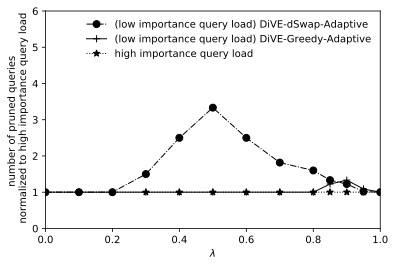
\includegraphics[ width=2.8in]{figures/results/low_vs_high}
	\caption{Number of pruned queries of high and low query load normalized by high query load using different value of $\lambda$, k = 5 and running on Heart disease dataset}
	\label{fig:low_vs_high}
\end{figure}

%
%\appendix
%%Appendix A
%\section{Headings in Appendices}
%The rules about hierarchical headings discussed above for
%the body of the article are different in the appendices.
%In the \textbf{appendix} environment, the command
%\textbf{section} is used to
%indicate the start of each Appendix, with alphabetic order
%designation (i.e., the first is A, the second B, etc.) and
%a title (if you include one).  So, if you need
%hierarchical structure
%\textit{within} an Appendix, start with \textbf{subsection} as the
%highest level. Here is an outline of the body of this
%document in Appendix-appropriate form:
%\subsection{Introduction}
%\subsection{The Body of the Paper}
%\subsubsection{Type Changes and  Special Characters}
%\subsubsection{Math Equations}
%\paragraph{Inline (In-text) Equations}
%\paragraph{Display Equations}
%\subsubsection{Citations}
%\subsubsection{Tables}
%\subsubsection{Figures}
%\subsubsection{Theorem-like Constructs}
%\subsubsection*{A Caveat for the \TeX\ Expert}
%\subsection{Conclusions}
%\subsection{References}
%Generated by bibtex from your \texttt{.bib} file.  Run latex,
%then bibtex, then latex twice (to resolve references)
%to create the \texttt{.bbl} file.  Insert that \texttt{.bbl}
%file into the \texttt{.tex} source file and comment out
%the command \texttt{{\char'134}thebibliography}.
% This next section command marks the start of
% Appendix B, and does not continue the present hierarchy
%\section{More Help for the Hardy}
%
%Of course, reading the source code is always useful.  The file
%\path{acmart.pdf} contains both the user guide and the commented
%code.

\begin{acks}
	This research is supported by the Indonesia Endowment Fund for Education (LPDP) as scholarship provider from the Ministry of Finance, Republic of Indonesia.
	Big thanks to Dr. Hina A Khan who help to fixing the gramatical error and giving the inputs to this work. 
	
\end{acks}


\bibliographystyle{ACM-Reference-Format}
\bibliography{cikm2018}

\end{document}
